% Options for packages loaded elsewhere
\PassOptionsToPackage{unicode}{hyperref}
\PassOptionsToPackage{hyphens}{url}
%
\documentclass[
]{book}
\usepackage{lmodern}
\usepackage{amssymb,amsmath}
\usepackage{ifxetex,ifluatex}
\ifnum 0\ifxetex 1\fi\ifluatex 1\fi=0 % if pdftex
  \usepackage[T1]{fontenc}
  \usepackage[utf8]{inputenc}
  \usepackage{textcomp} % provide euro and other symbols
\else % if luatex or xetex
  \usepackage{unicode-math}
  \defaultfontfeatures{Scale=MatchLowercase}
  \defaultfontfeatures[\rmfamily]{Ligatures=TeX,Scale=1}
  \setmainfont[]{Arial}
  \setmonofont[]{Courier New}
\fi
% Use upquote if available, for straight quotes in verbatim environments
\IfFileExists{upquote.sty}{\usepackage{upquote}}{}
\IfFileExists{microtype.sty}{% use microtype if available
  \usepackage[]{microtype}
  \UseMicrotypeSet[protrusion]{basicmath} % disable protrusion for tt fonts
}{}
\makeatletter
\@ifundefined{KOMAClassName}{% if non-KOMA class
  \IfFileExists{parskip.sty}{%
    \usepackage{parskip}
  }{% else
    \setlength{\parindent}{0pt}
    \setlength{\parskip}{6pt plus 2pt minus 1pt}}
}{% if KOMA class
  \KOMAoptions{parskip=half}}
\makeatother
\usepackage{xcolor}
\IfFileExists{xurl.sty}{\usepackage{xurl}}{} % add URL line breaks if available
\IfFileExists{bookmark.sty}{\usepackage{bookmark}}{\usepackage{hyperref}}
\hypersetup{
  pdftitle={STAT 107 Outline of Class Notes},
  pdfauthor={Rebecca Kurtz-Garcia},
  hidelinks,
  pdfcreator={LaTeX via pandoc}}
\urlstyle{same} % disable monospaced font for URLs
\usepackage{color}
\usepackage{fancyvrb}
\newcommand{\VerbBar}{|}
\newcommand{\VERB}{\Verb[commandchars=\\\{\}]}
\DefineVerbatimEnvironment{Highlighting}{Verbatim}{commandchars=\\\{\}}
% Add ',fontsize=\small' for more characters per line
\usepackage{framed}
\definecolor{shadecolor}{RGB}{248,248,248}
\newenvironment{Shaded}{\begin{snugshade}}{\end{snugshade}}
\newcommand{\AlertTok}[1]{\textcolor[rgb]{0.94,0.16,0.16}{#1}}
\newcommand{\AnnotationTok}[1]{\textcolor[rgb]{0.56,0.35,0.01}{\textbf{\textit{#1}}}}
\newcommand{\AttributeTok}[1]{\textcolor[rgb]{0.77,0.63,0.00}{#1}}
\newcommand{\BaseNTok}[1]{\textcolor[rgb]{0.00,0.00,0.81}{#1}}
\newcommand{\BuiltInTok}[1]{#1}
\newcommand{\CharTok}[1]{\textcolor[rgb]{0.31,0.60,0.02}{#1}}
\newcommand{\CommentTok}[1]{\textcolor[rgb]{0.56,0.35,0.01}{\textit{#1}}}
\newcommand{\CommentVarTok}[1]{\textcolor[rgb]{0.56,0.35,0.01}{\textbf{\textit{#1}}}}
\newcommand{\ConstantTok}[1]{\textcolor[rgb]{0.00,0.00,0.00}{#1}}
\newcommand{\ControlFlowTok}[1]{\textcolor[rgb]{0.13,0.29,0.53}{\textbf{#1}}}
\newcommand{\DataTypeTok}[1]{\textcolor[rgb]{0.13,0.29,0.53}{#1}}
\newcommand{\DecValTok}[1]{\textcolor[rgb]{0.00,0.00,0.81}{#1}}
\newcommand{\DocumentationTok}[1]{\textcolor[rgb]{0.56,0.35,0.01}{\textbf{\textit{#1}}}}
\newcommand{\ErrorTok}[1]{\textcolor[rgb]{0.64,0.00,0.00}{\textbf{#1}}}
\newcommand{\ExtensionTok}[1]{#1}
\newcommand{\FloatTok}[1]{\textcolor[rgb]{0.00,0.00,0.81}{#1}}
\newcommand{\FunctionTok}[1]{\textcolor[rgb]{0.00,0.00,0.00}{#1}}
\newcommand{\ImportTok}[1]{#1}
\newcommand{\InformationTok}[1]{\textcolor[rgb]{0.56,0.35,0.01}{\textbf{\textit{#1}}}}
\newcommand{\KeywordTok}[1]{\textcolor[rgb]{0.13,0.29,0.53}{\textbf{#1}}}
\newcommand{\NormalTok}[1]{#1}
\newcommand{\OperatorTok}[1]{\textcolor[rgb]{0.81,0.36,0.00}{\textbf{#1}}}
\newcommand{\OtherTok}[1]{\textcolor[rgb]{0.56,0.35,0.01}{#1}}
\newcommand{\PreprocessorTok}[1]{\textcolor[rgb]{0.56,0.35,0.01}{\textit{#1}}}
\newcommand{\RegionMarkerTok}[1]{#1}
\newcommand{\SpecialCharTok}[1]{\textcolor[rgb]{0.00,0.00,0.00}{#1}}
\newcommand{\SpecialStringTok}[1]{\textcolor[rgb]{0.31,0.60,0.02}{#1}}
\newcommand{\StringTok}[1]{\textcolor[rgb]{0.31,0.60,0.02}{#1}}
\newcommand{\VariableTok}[1]{\textcolor[rgb]{0.00,0.00,0.00}{#1}}
\newcommand{\VerbatimStringTok}[1]{\textcolor[rgb]{0.31,0.60,0.02}{#1}}
\newcommand{\WarningTok}[1]{\textcolor[rgb]{0.56,0.35,0.01}{\textbf{\textit{#1}}}}
\usepackage{longtable,booktabs}
% Correct order of tables after \paragraph or \subparagraph
\usepackage{etoolbox}
\makeatletter
\patchcmd\longtable{\par}{\if@noskipsec\mbox{}\fi\par}{}{}
\makeatother
% Allow footnotes in longtable head/foot
\IfFileExists{footnotehyper.sty}{\usepackage{footnotehyper}}{\usepackage{footnote}}
\makesavenoteenv{longtable}
\usepackage{graphicx,grffile}
\makeatletter
\def\maxwidth{\ifdim\Gin@nat@width>\linewidth\linewidth\else\Gin@nat@width\fi}
\def\maxheight{\ifdim\Gin@nat@height>\textheight\textheight\else\Gin@nat@height\fi}
\makeatother
% Scale images if necessary, so that they will not overflow the page
% margins by default, and it is still possible to overwrite the defaults
% using explicit options in \includegraphics[width, height, ...]{}
\setkeys{Gin}{width=\maxwidth,height=\maxheight,keepaspectratio}
% Set default figure placement to htbp
\makeatletter
\def\fps@figure{htbp}
\makeatother
\setlength{\emergencystretch}{3em} % prevent overfull lines
\providecommand{\tightlist}{%
  \setlength{\itemsep}{0pt}\setlength{\parskip}{0pt}}
\setcounter{secnumdepth}{5}
\usepackage{booktabs}
\usepackage[]{natbib}
\bibliographystyle{plainnat}

\title{STAT 107 Outline of Class Notes}
\author{Rebecca Kurtz-Garcia}
\date{2021-09-19}

\begin{document}
\maketitle

{
\setcounter{tocdepth}{1}
\tableofcontents
}
\hypertarget{welcome}{%
\chapter*{Welcome}\label{welcome}}
\addcontentsline{toc}{chapter}{Welcome}

Welcome to STAT 107! Here is stuff that can be written.

\hypertarget{introduction-to-r}{%
\chapter{Introduction to R}\label{introduction-to-r}}

This section was written primarily by \citet{Desharnais2020}, and was modified for our course. I am grateful for his help.

\hypertarget{the-rstudio-interface}{%
\section{\texorpdfstring{The \textbf{RStudio} Interface}{The RStudio Interface}}\label{the-rstudio-interface}}

We will begin by looking at the RStudio software interface. Refer to Figure 1 as you follow the instructions below.

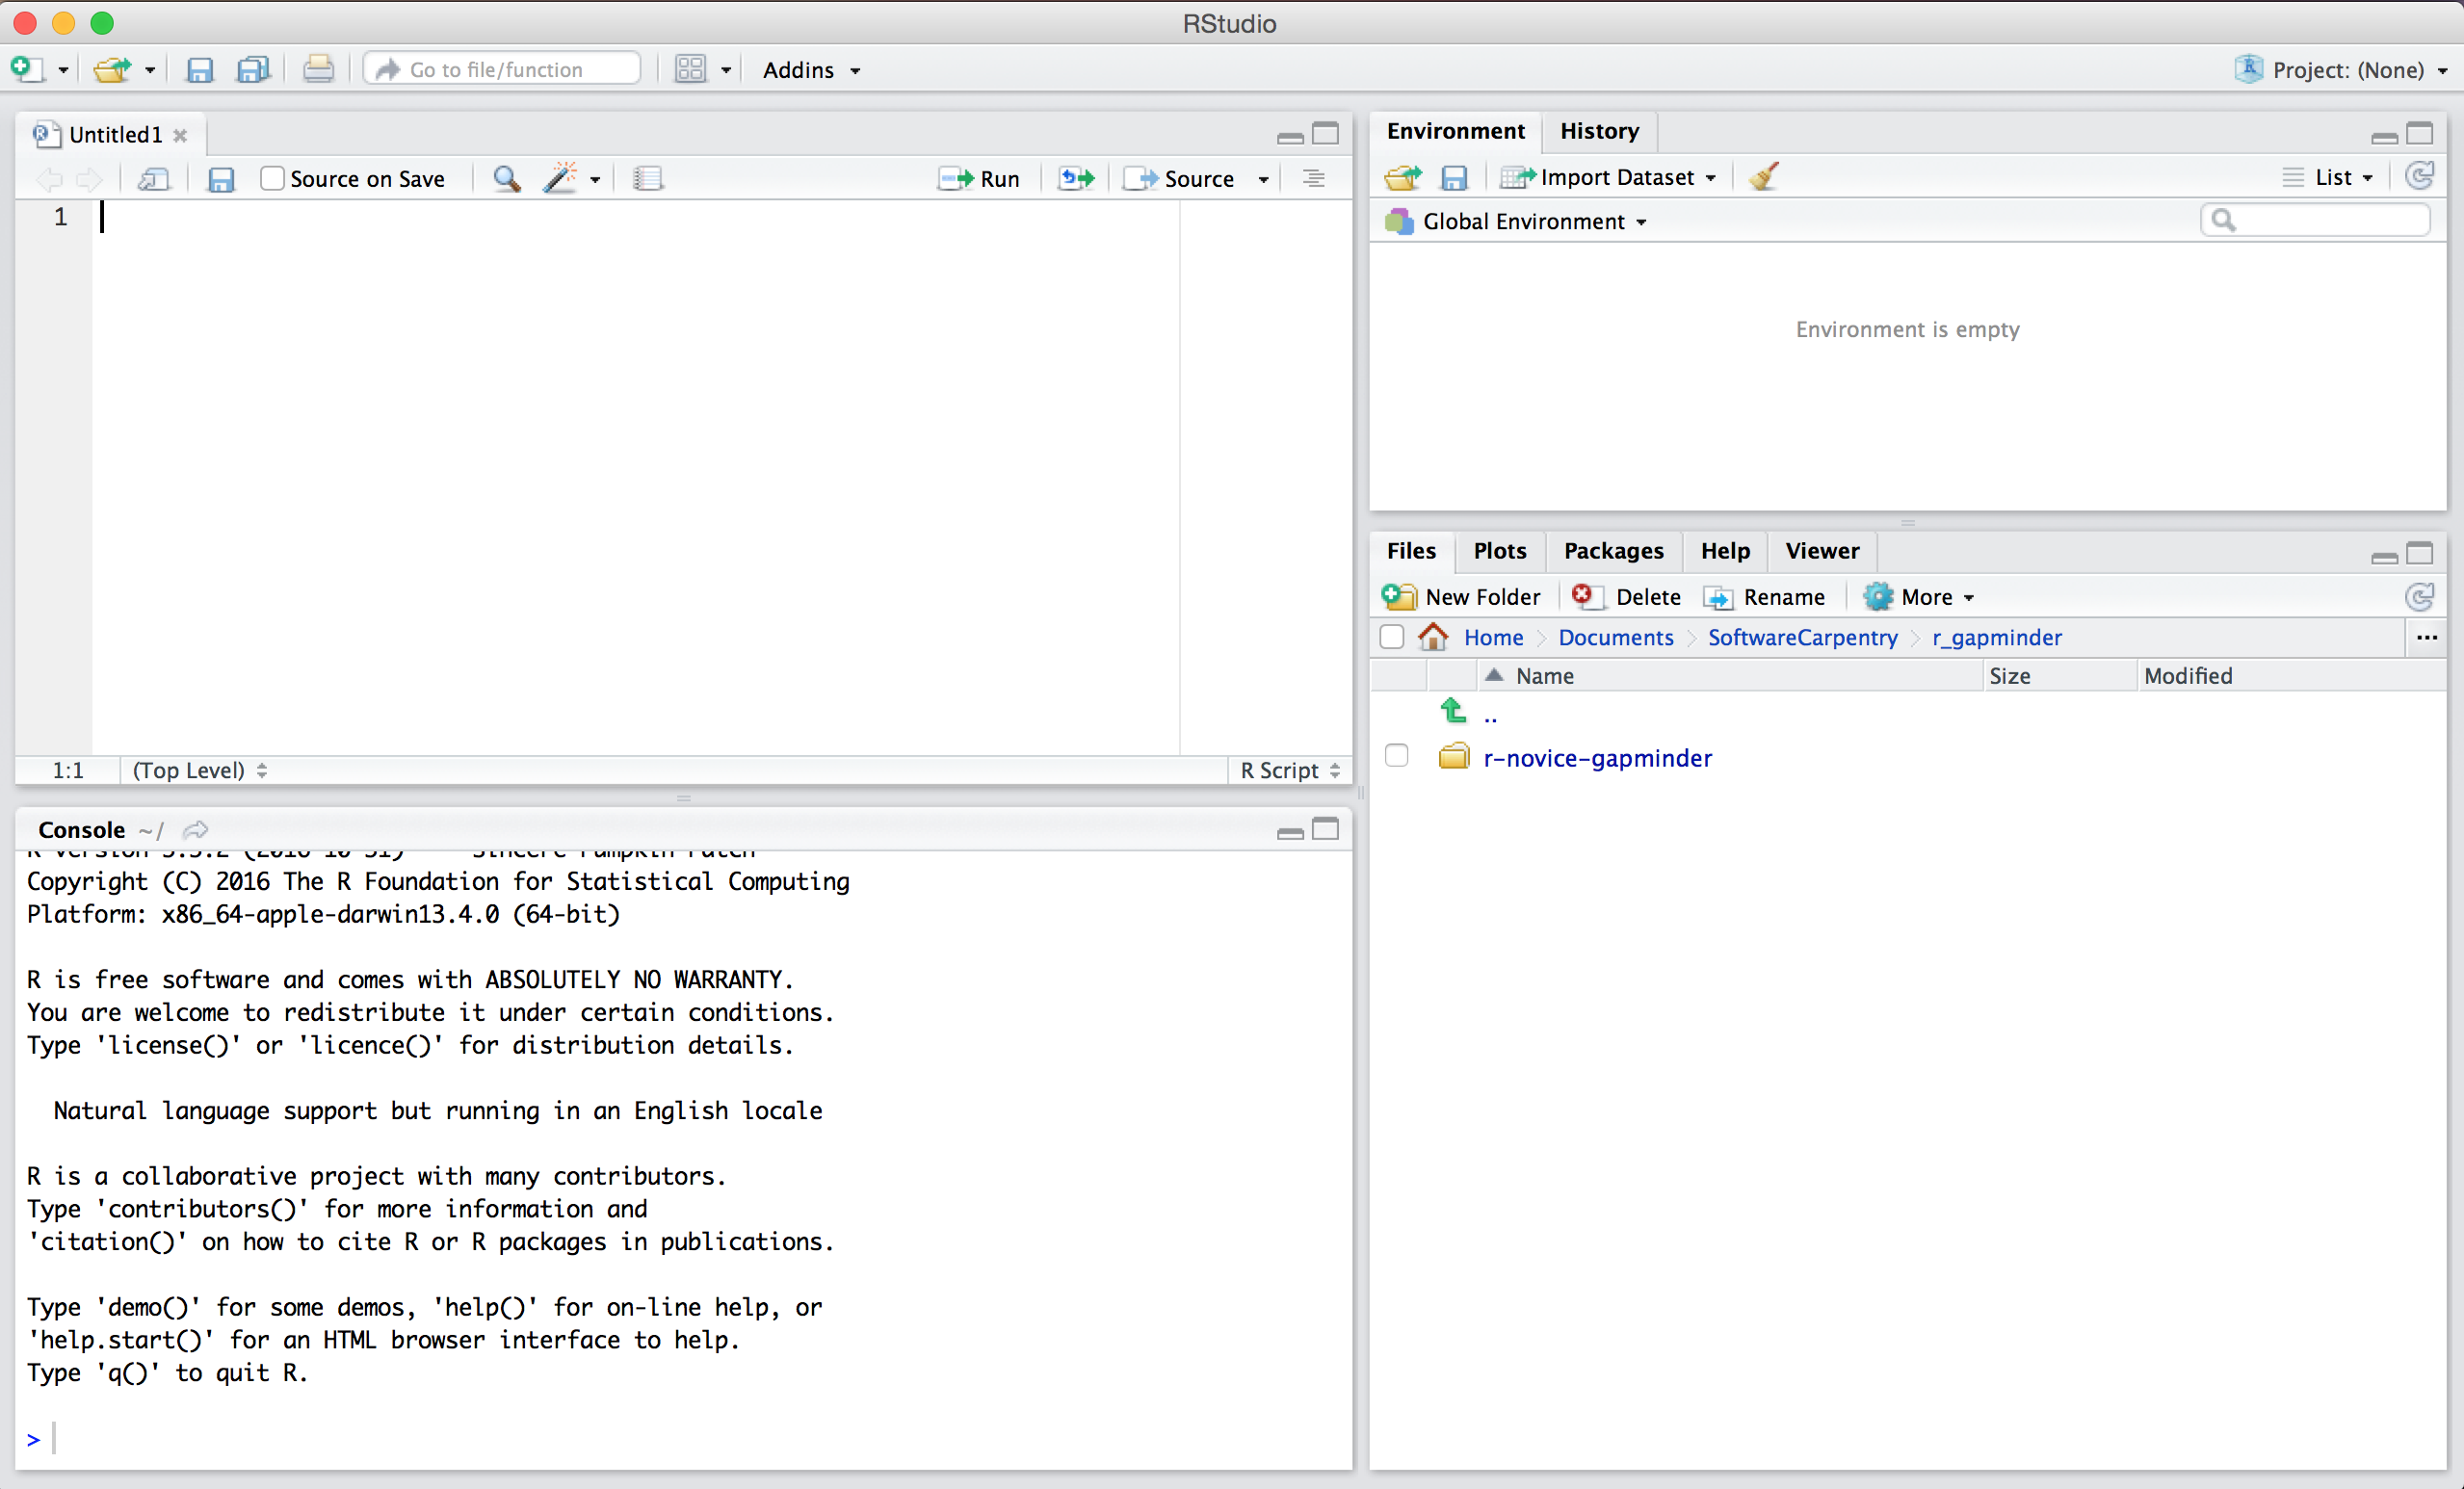
\includegraphics[width=35.53in]{images/rstudio}

Launch RStudio. You will see a window that looks like Fig. 1. There are four panels of the window:

\begin{itemize}
\item
  The R Command Console is where you type R commands for immediate execution.
\item
  The Notebook in the upper left portion of the window is an area for editing R source code for scripts and functions and for viewing R data frame objects. New tabs will be added as new R code files and data objects are opened.
\item
  The Notebook in the upper right portion of the window is an area for browsing the variables in the R workspace environment and the R command line history.
\item
  The Notebook in the lower right portion of the window has several tabs. The Files tab is an area for browsing the files in the current working directory. The Plot tab is for viewing graphics produced using R commands. The Packages tab lists the R packages available. Other packages can be loaded. The Help tab provides access to the R documentation. The Viewer tab is for viewing local web content in the temporary session directory (not files on the web).
\end{itemize}

\hypertarget{bottom-left-pane}{%
\subsection*{Bottom Left Pane}\label{bottom-left-pane}}
\addcontentsline{toc}{subsection}{Bottom Left Pane}

Let's begin with the Console. This is where you type \texttt{R} commands for immediate execution. Click in the Command Console, ``\textgreater{}'' symbol is the system prompt. You should see a blinking cursor that tells you the console is the current focus of keyboard input. Type:

\begin{Shaded}
\begin{Highlighting}[]
\DecValTok{1}\OperatorTok{+}\DecValTok{2}
\end{Highlighting}
\end{Shaded}

\begin{verbatim}
## [1] 3
\end{verbatim}

The result tells you that the line begins with the first (and only) element of the result which is the number 3. You can also execute R's built-in functions (or functions you add). Type the following command.

\begin{Shaded}
\begin{Highlighting}[]
\KeywordTok{exp}\NormalTok{(pi)}
\end{Highlighting}
\end{Shaded}

\begin{verbatim}
## [1] 23.14069
\end{verbatim}

In \texttt{R}, ``pi'' is a special constant to represent the number and ``exp'' is the exponential function. The result tells you that the first (and only) element of the result is the number \(e^{\pi}=\) 23.14069.

\hypertarget{bottom-right-pane}{%
\subsection*{Bottom Right Pane}\label{bottom-right-pane}}
\addcontentsline{toc}{subsection}{Bottom Right Pane}

Now let's look at the \emph{Files} tab of the notebook at the lower right of the window. Every \texttt{R} session has a working directory where \texttt{R} looks for and saves files. It is a good practice to create a different directory for every project and make that directory the working directory. For example, let's make a new directory called \emph{MyDirectory}. (You can chose another name if you wish).

\begin{enumerate}
\def\labelenumi{\arabic{enumi})}
\item
  Click on the \textbf{Files} tab of the notebook. You should see a listing of files in your default working directory.
\item
  Click on the small button with an ellipsis image on the right side of the file path above the directory listing.
\item
  Navigate to the folder where you want to create the new directory and click the \textbf{OK} button.
\item
  Click on the \textbf{New Folder} button just below the Files tab (see right).
\item
  Type \textbf{MyDirectory} in the panel that opens click on the folder in the Notebook.
\item
  Click the \textbf{More} button to the right of the New Folder button and select the menu option \textbf{Set as Working Directory}. This new folder is now the working directory for the current R session. This menu option is a short cut for a command that was automatically entered into the R console.
\end{enumerate}

\hypertarget{top-right-pane}{%
\subsection*{Top Right Pane}\label{top-right-pane}}
\addcontentsline{toc}{subsection}{Top Right Pane}

Next we will look at the \emph{R environment}, also called the \emph{R workspace}. This is where you can see the names and other information on the variables that were created during your \texttt{R} session and are available for use in other commands.

In the \texttt{R} console type:

\begin{Shaded}
\begin{Highlighting}[]
\NormalTok{a =}\StringTok{ }\FloatTok{29.325}
\NormalTok{b =}\StringTok{ }\KeywordTok{log}\NormalTok{(a)}
\NormalTok{c =}\StringTok{ }\NormalTok{a}\OperatorTok{/}\NormalTok{b}
\end{Highlighting}
\end{Shaded}

Look at the Environment pane. The variables \texttt{a}, \texttt{b}, and \texttt{c} are now part of your R work space. You can reuse those variables as part of other commands.

In the \texttt{R} console type:

\begin{Shaded}
\begin{Highlighting}[]
\NormalTok{v=}\StringTok{ }\KeywordTok{c}\NormalTok{(a, b, c)}
\NormalTok{v}
\end{Highlighting}
\end{Shaded}

\begin{verbatim}
## [1] 29.325000  3.378440  8.680041
\end{verbatim}

The variable \texttt{v} is a vector created using the \emph{concatenate} function \texttt{c()}. (The concatenate should not be confused with the variable c that was created earlier. Functions are always followed by parentheses that contain the function arguments.) This function combines its arguments into a vector or list. Look at the Environment panel. The text \texttt{num\ {[}1:3{]}} tells us that the variable \texttt{v} is a vector with elements \texttt{v{[}1{]}}, \texttt{v{[}2{]}}, and \texttt{v{[}3{]}}.

\hypertarget{top-left-pane}{%
\subsection*{Top Left Pane}\label{top-left-pane}}
\addcontentsline{toc}{subsection}{Top Left Pane}

Now let's look at the \texttt{R} viewer notebook. This panel can be used to data which are data frame objects or \emph{matrix objects} in \texttt{R}.

We will begin by taking advantage of a data frame object that was built into \texttt{R} for demonstration purposes. We will copy it into a data frame object. In the \texttt{R} console, type:

\begin{Shaded}
\begin{Highlighting}[]
\NormalTok{df =}\StringTok{ }\NormalTok{mtcars}
\end{Highlighting}
\end{Shaded}

Let's view the data. On the right side of the entry for the \texttt{df} object is a button we can use to view the entries of the data frame (see green arrow below). Click on the View Button.

If your look in the notebook area in the upper left portion of the window, you can see a spreadsheet-like view of the data. This is for viewing only; you cannot edit the data. Use the scroll bars to view the data entries.

You can also list the data in the console by typing the name of the data fame object:

\begin{Shaded}
\begin{Highlighting}[]
\NormalTok{df}
\end{Highlighting}
\end{Shaded}

\begin{verbatim}
##                      mpg cyl  disp  hp drat    wt  qsec vs am gear carb
## Mazda RX4           21.0   6 160.0 110 3.90 2.620 16.46  0  1    4    4
## Mazda RX4 Wag       21.0   6 160.0 110 3.90 2.875 17.02  0  1    4    4
## Datsun 710          22.8   4 108.0  93 3.85 2.320 18.61  1  1    4    1
## Hornet 4 Drive      21.4   6 258.0 110 3.08 3.215 19.44  1  0    3    1
## Hornet Sportabout   18.7   8 360.0 175 3.15 3.440 17.02  0  0    3    2
## Valiant             18.1   6 225.0 105 2.76 3.460 20.22  1  0    3    1
## Duster 360          14.3   8 360.0 245 3.21 3.570 15.84  0  0    3    4
## Merc 240D           24.4   4 146.7  62 3.69 3.190 20.00  1  0    4    2
## Merc 230            22.8   4 140.8  95 3.92 3.150 22.90  1  0    4    2
## Merc 280            19.2   6 167.6 123 3.92 3.440 18.30  1  0    4    4
## Merc 280C           17.8   6 167.6 123 3.92 3.440 18.90  1  0    4    4
## Merc 450SE          16.4   8 275.8 180 3.07 4.070 17.40  0  0    3    3
## Merc 450SL          17.3   8 275.8 180 3.07 3.730 17.60  0  0    3    3
## Merc 450SLC         15.2   8 275.8 180 3.07 3.780 18.00  0  0    3    3
## Cadillac Fleetwood  10.4   8 472.0 205 2.93 5.250 17.98  0  0    3    4
## Lincoln Continental 10.4   8 460.0 215 3.00 5.424 17.82  0  0    3    4
## Chrysler Imperial   14.7   8 440.0 230 3.23 5.345 17.42  0  0    3    4
## Fiat 128            32.4   4  78.7  66 4.08 2.200 19.47  1  1    4    1
## Honda Civic         30.4   4  75.7  52 4.93 1.615 18.52  1  1    4    2
## Toyota Corolla      33.9   4  71.1  65 4.22 1.835 19.90  1  1    4    1
## Toyota Corona       21.5   4 120.1  97 3.70 2.465 20.01  1  0    3    1
## Dodge Challenger    15.5   8 318.0 150 2.76 3.520 16.87  0  0    3    2
## AMC Javelin         15.2   8 304.0 150 3.15 3.435 17.30  0  0    3    2
## Camaro Z28          13.3   8 350.0 245 3.73 3.840 15.41  0  0    3    4
## Pontiac Firebird    19.2   8 400.0 175 3.08 3.845 17.05  0  0    3    2
## Fiat X1-9           27.3   4  79.0  66 4.08 1.935 18.90  1  1    4    1
## Porsche 914-2       26.0   4 120.3  91 4.43 2.140 16.70  0  1    5    2
## Lotus Europa        30.4   4  95.1 113 3.77 1.513 16.90  1  1    5    2
## Ford Pantera L      15.8   8 351.0 264 4.22 3.170 14.50  0  1    5    4
## Ferrari Dino        19.7   6 145.0 175 3.62 2.770 15.50  0  1    5    6
## Maserati Bora       15.0   8 301.0 335 3.54 3.570 14.60  0  1    5    8
## Volvo 142E          21.4   4 121.0 109 4.11 2.780 18.60  1  1    4    2
\end{verbatim}

The columns are labeled with the names of the variables and the rows are labeled with the names of each car. Each row represents the data values for one car; that is, each row is one observation.

\hypertarget{comments}{%
\section{Comments}\label{comments}}

Often times we will want to add a comment to our script document so we can remember special aspects later, and make the code easier to read and modify in the future. To add a comment start the comment with a \texttt{\#} symbol. This will make the remaining characters in a line a comment and R will not try to compile these lines. Go to the script document and type the following. Highlight what you have typed and press ``Run''.

\begin{Shaded}
\begin{Highlighting}[]
\CommentTok{# This is a comment }
\DecValTok{2}\OperatorTok{+}\StringTok{ }\DecValTok{2}
\end{Highlighting}
\end{Shaded}

\begin{verbatim}
## [1] 4
\end{verbatim}

\begin{Shaded}
\begin{Highlighting}[]
\DecValTok{2} \OperatorTok{+}\StringTok{ }\DecValTok{3} \CommentTok{# Comments can also start in the middle of a line. }
\end{Highlighting}
\end{Shaded}

\begin{verbatim}
## [1] 5
\end{verbatim}

\hypertarget{operators}{%
\section{Operators}\label{operators}}

An operator is a symbol that tells the compiler to preform a specific task. There are several types of operators, some preeform mathematical tasks, logical checks, and create new objects. We will review a few of the basic operators here. We will continue to discuss and introduce operators throughout this document.

\hypertarget{arithmetic-operators}{%
\subsection*{Arithmetic Operators}\label{arithmetic-operators}}
\addcontentsline{toc}{subsection}{Arithmetic Operators}

R was designed for statistical applications and as a necessity it needs to preform mathematical operations efficiently and effectively. The first operators we discuss are a few of the basic arithmetic operations. These are operations ismilar to that of a calculator.

\begin{Shaded}
\begin{Highlighting}[]
\CommentTok{# Addition }
\DecValTok{2}\OperatorTok{+}\StringTok{ }\DecValTok{3}
\end{Highlighting}
\end{Shaded}

\begin{verbatim}
## [1] 5
\end{verbatim}

\begin{Shaded}
\begin{Highlighting}[]
\CommentTok{# Subtraction }
\DecValTok{2} \OperatorTok{-}\StringTok{ }\DecValTok{3}
\end{Highlighting}
\end{Shaded}

\begin{verbatim}
## [1] -1
\end{verbatim}

\begin{Shaded}
\begin{Highlighting}[]
\CommentTok{# Multiplication }
\DecValTok{2}\OperatorTok{*}\DecValTok{3}
\end{Highlighting}
\end{Shaded}

\begin{verbatim}
## [1] 6
\end{verbatim}

\begin{Shaded}
\begin{Highlighting}[]
\CommentTok{# Division }
\DecValTok{2}\OperatorTok{/}\DecValTok{3}
\end{Highlighting}
\end{Shaded}

\begin{verbatim}
## [1] 0.6666667
\end{verbatim}

\begin{Shaded}
\begin{Highlighting}[]
\CommentTok{# Exponent }
\DecValTok{2}\OperatorTok{^}\DecValTok{3}
\end{Highlighting}
\end{Shaded}

\begin{verbatim}
## [1] 8
\end{verbatim}

\hypertarget{relational-operators}{%
\subsection*{Relational Operators}\label{relational-operators}}
\addcontentsline{toc}{subsection}{Relational Operators}

Relational operators are used to compare two values. When using a relational operation R will return either \texttt{TRUE} or \texttt{FALSE}.

\begin{Shaded}
\begin{Highlighting}[]
\CommentTok{# Less than }
\DecValTok{2} \OperatorTok{<}\StringTok{ }\DecValTok{3}
\end{Highlighting}
\end{Shaded}

\begin{verbatim}
## [1] TRUE
\end{verbatim}

\begin{Shaded}
\begin{Highlighting}[]
\CommentTok{# Greater than }
\DecValTok{2} \OperatorTok{>}\StringTok{ }\DecValTok{3}
\end{Highlighting}
\end{Shaded}

\begin{verbatim}
## [1] FALSE
\end{verbatim}

\begin{Shaded}
\begin{Highlighting}[]
\CommentTok{# Less than or equal to }
\DecValTok{2} \OperatorTok{<=}\StringTok{ }\DecValTok{3}
\end{Highlighting}
\end{Shaded}

\begin{verbatim}
## [1] TRUE
\end{verbatim}

\begin{Shaded}
\begin{Highlighting}[]
\CommentTok{# Greater than or equal to }
\DecValTok{2}\OperatorTok{>=}\StringTok{ }\DecValTok{3}
\end{Highlighting}
\end{Shaded}

\begin{verbatim}
## [1] FALSE
\end{verbatim}

\begin{Shaded}
\begin{Highlighting}[]
\CommentTok{# Not equal to }
\DecValTok{2} \OperatorTok{!=}\StringTok{ }\DecValTok{3}
\end{Highlighting}
\end{Shaded}

\begin{verbatim}
## [1] TRUE
\end{verbatim}

\begin{Shaded}
\begin{Highlighting}[]
\CommentTok{# Equal to }
\DecValTok{2} \OperatorTok{==}\StringTok{ }\DecValTok{3}
\end{Highlighting}
\end{Shaded}

\begin{verbatim}
## [1] FALSE
\end{verbatim}

We can use all the same operators above if our object contains more than one element. This will preform the above comparisons element by element.

\begin{Shaded}
\begin{Highlighting}[]
\NormalTok{v}
\end{Highlighting}
\end{Shaded}

\begin{verbatim}
## [1] 29.325000  3.378440  8.680041
\end{verbatim}

\begin{Shaded}
\begin{Highlighting}[]
\NormalTok{v }\OperatorTok{>}\StringTok{ }\DecValTok{10}
\end{Highlighting}
\end{Shaded}

\begin{verbatim}
## [1]  TRUE FALSE FALSE
\end{verbatim}

If we have two vectors of an unequal length then the checks will be preformed element-by-element but the values in the shorter vector will be \emph{recycled}, or \emph{repeated}.

\begin{Shaded}
\begin{Highlighting}[]
\NormalTok{w =}\StringTok{ }\KeywordTok{c}\NormalTok{(}\DecValTok{10}\NormalTok{, }\DecValTok{1}\NormalTok{)}
\NormalTok{v }\OperatorTok{>}\StringTok{ }\NormalTok{w}
\end{Highlighting}
\end{Shaded}

\begin{verbatim}
## Warning in v > w: longer object length is not a multiple of shorter object
## length
\end{verbatim}

\begin{verbatim}
## [1]  TRUE  TRUE FALSE
\end{verbatim}

R evaluated the first and third element of \texttt{v} and compared it to the first element of \texttt{w}, and the second element of \texttt{v} to the second element of \texttt{w}. In this case, R returned a \emph{warning} alerting you that it recycled elements. However, R will not always do this.

\hypertarget{logical-operators}{%
\subsection*{Logical operators}\label{logical-operators}}
\addcontentsline{toc}{subsection}{Logical operators}

Logical operators are similar to relational operators. They are used to check ``AND'' and ``OR'' events. We have the \texttt{\&} symbol which returns \texttt{TRUE} only if BOTH conditions are true. We also have the \texttt{\textbar{}} symbol which returns \texttt{TRUE} if EITHER condition is true.

\begin{Shaded}
\begin{Highlighting}[]
\CommentTok{# Check if both operations are true. }
\NormalTok{(}\DecValTok{2} \OperatorTok{<}\StringTok{ }\DecValTok{3}\NormalTok{) }\OperatorTok{&}\StringTok{ }\NormalTok{(}\DecValTok{5} \OperatorTok{<}\StringTok{ }\DecValTok{4}\NormalTok{)}
\end{Highlighting}
\end{Shaded}

\begin{verbatim}
## [1] FALSE
\end{verbatim}

\begin{Shaded}
\begin{Highlighting}[]
\CommentTok{# Check if either operation is true. }
\NormalTok{(}\DecValTok{2} \OperatorTok{<}\StringTok{ }\DecValTok{3}\NormalTok{) }\OperatorTok{|}\StringTok{ }\NormalTok{(}\DecValTok{5} \OperatorTok{<}\StringTok{ }\DecValTok{4}\NormalTok{)}
\end{Highlighting}
\end{Shaded}

\begin{verbatim}
## [1] TRUE
\end{verbatim}

We can also negate a \texttt{TRUE} or \texttt{FALSE} value using the \texttt{!} symbol.

\begin{Shaded}
\begin{Highlighting}[]
\CommentTok{# Negate an operation }
\OperatorTok{!}\NormalTok{(}\DecValTok{2}\OperatorTok{<}\DecValTok{3}\NormalTok{) }
\end{Highlighting}
\end{Shaded}

\begin{verbatim}
## [1] FALSE
\end{verbatim}

Like relational operators from before, if we have more than one element the logical operations will be implemented element-by-element.

\begin{Shaded}
\begin{Highlighting}[]
\CommentTok{# AND event, compared element-by-element}
\NormalTok{(v }\OperatorTok{>}\StringTok{ }\DecValTok{10}\NormalTok{) }\OperatorTok{&}\StringTok{ }\NormalTok{(}\DecValTok{4} \OperatorTok{<}\StringTok{ }\DecValTok{5}\NormalTok{) }
\end{Highlighting}
\end{Shaded}

\begin{verbatim}
## [1]  TRUE FALSE FALSE
\end{verbatim}

\begin{Shaded}
\begin{Highlighting}[]
\CommentTok{# OR event, compared elmeent-by-elment}
\NormalTok{(v }\OperatorTok{>}\StringTok{ }\DecValTok{10}\NormalTok{) }\OperatorTok{|}\StringTok{ }\NormalTok{(}\DecValTok{4} \OperatorTok{<}\StringTok{ }\DecValTok{5}\NormalTok{) }
\end{Highlighting}
\end{Shaded}

\begin{verbatim}
## [1] TRUE TRUE TRUE
\end{verbatim}

We also have the symbols \texttt{\&\&} and \texttt{\textbar{}\textbar{}} which will ensure that only the first element in an object will be compared.

\begin{Shaded}
\begin{Highlighting}[]
\CommentTok{# AND event, only check the first element}
\NormalTok{(v }\OperatorTok{>}\StringTok{ }\DecValTok{10}\NormalTok{) }\OperatorTok{&&}\StringTok{ }\NormalTok{(}\DecValTok{4} \OperatorTok{<}\StringTok{ }\DecValTok{5}\NormalTok{) }
\end{Highlighting}
\end{Shaded}

\begin{verbatim}
## [1] TRUE
\end{verbatim}

\begin{Shaded}
\begin{Highlighting}[]
\CommentTok{# OR event, only check the first element}
\NormalTok{(v }\OperatorTok{>}\StringTok{ }\DecValTok{10}\NormalTok{) }\OperatorTok{||}\StringTok{ }\NormalTok{(}\DecValTok{4} \OperatorTok{<}\StringTok{ }\DecValTok{5}\NormalTok{) }
\end{Highlighting}
\end{Shaded}

\begin{verbatim}
## [1] TRUE
\end{verbatim}

\hypertarget{assignment-operators}{%
\subsection*{Assignment Operators}\label{assignment-operators}}
\addcontentsline{toc}{subsection}{Assignment Operators}

Assignment operators are used to assign values to a new object. There are many types of assignment operators, and they operate slightly differently. The two most common assignment operators are \texttt{=} and \texttt{\textless{}-}. With these operators the value to the left of the operator is the name of the new object and the value on the right is what the object is now equal to.

\begin{Shaded}
\begin{Highlighting}[]
\NormalTok{x =}\StringTok{ }\DecValTok{5}
\NormalTok{x}
\end{Highlighting}
\end{Shaded}

\begin{verbatim}
## [1] 5
\end{verbatim}

\begin{Shaded}
\begin{Highlighting}[]
\NormalTok{x <-}\StringTok{ }\DecValTok{5}
\NormalTok{x}
\end{Highlighting}
\end{Shaded}

\begin{verbatim}
## [1] 5
\end{verbatim}

The majority of the time we can use these two assignment operators above interchangeably, there are some exceptions though. There are several other assignment operators which are uncommon and should only be used by advanced users, \texttt{-\textgreater{}}, \texttt{\textless{}\textless{}-}, and \texttt{-\textgreater{}\textgreater{}}.

\hypertarget{additional-resources}{%
\section{Additional Resources}\label{additional-resources}}

\begin{itemize}
\tightlist
\item
  Chapters 1 of \href{https://cran.r-project.org/doc/manuals/r-release/R-intro.pdf}{CRAN Intro-to-R Manual}
\item
  Videos:

  \begin{itemize}
  \tightlist
  \item
    \href{https://ucr.yuja.com/V/Video?v=2365045\&node=8476457\&a=437885577\&autoplay=1}{Getting Started 1 \textbar{} How to Download and Install RStudio}
  \item
    \href{https://ucr.yuja.com/V/Video?v=2368643\&node=8487538\&a=437248619\&autoplay=1}{Getting Started 2 \textbar{} Rstudio Introduction cont'd, More Tabs Explained}
  \end{itemize}
\end{itemize}

\hypertarget{introduction-to-r-objects}{%
\chapter{Introduction to R Objects}\label{introduction-to-r-objects}}

\hypertarget{atomic-objects}{%
\section{Atomic Objects}\label{atomic-objects}}

At its core, R is an objected-oriented computational and programming environment. Everything in R is an object belonging to a certain \emph{class}.
R can represent different types of data. The types include \texttt{numeric}, \texttt{integer}, \texttt{complex}, \texttt{logical}, \texttt{character}, and \texttt{raw}. These are the basic fundamental objects we can use in R. In practice \texttt{raw} is rarely used. For our class we will not need the \texttt{complex} type which stores complex numbers. Unlike other object-oriented languages we do not need to specify what type of object we are creating. Instead, R guesses the type of object you are creating. To check the object type we can use the \texttt{class()} function. function.

\hypertarget{numeric}{%
\subsection*{Numeric}\label{numeric}}
\addcontentsline{toc}{subsection}{Numeric}

Numeric objects are perhaps the most common. These are objects which contain a real number, that is, a number which can contain a decimal value. These objects are comparable to \texttt{doubles} in \texttt{C}.

\begin{Shaded}
\begin{Highlighting}[]
\NormalTok{a =}\StringTok{ }\FloatTok{17.45}
\NormalTok{a}
\end{Highlighting}
\end{Shaded}

\begin{verbatim}
## [1] 17.45
\end{verbatim}

\begin{Shaded}
\begin{Highlighting}[]
\KeywordTok{class}\NormalTok{(a)}
\end{Highlighting}
\end{Shaded}

\begin{verbatim}
## [1] "numeric"
\end{verbatim}

\begin{Shaded}
\begin{Highlighting}[]
\NormalTok{b =}\StringTok{ }\DecValTok{5}
\NormalTok{b }
\end{Highlighting}
\end{Shaded}

\begin{verbatim}
## [1] 5
\end{verbatim}

\begin{Shaded}
\begin{Highlighting}[]
\KeywordTok{class}\NormalTok{(b)}
\end{Highlighting}
\end{Shaded}

\begin{verbatim}
## [1] "numeric"
\end{verbatim}

Both the variables \texttt{a} and \texttt{b} are \texttt{numeric} objects. When you type a number \texttt{R} will default to treating it as a \texttt{numeric} object which allows decimals.

\hypertarget{integer}{%
\subsection*{Integer}\label{integer}}
\addcontentsline{toc}{subsection}{Integer}

We can also create numeric objects which are specifically made to store integer values. We can do this using the \texttt{as.integer()} function.

\begin{Shaded}
\begin{Highlighting}[]
\NormalTok{a =}\StringTok{ }\KeywordTok{as.integer}\NormalTok{(a)}
\NormalTok{a}
\end{Highlighting}
\end{Shaded}

\begin{verbatim}
## [1] 17
\end{verbatim}

\begin{Shaded}
\begin{Highlighting}[]
\KeywordTok{class}\NormalTok{(a)}
\end{Highlighting}
\end{Shaded}

\begin{verbatim}
## [1] "integer"
\end{verbatim}

\begin{Shaded}
\begin{Highlighting}[]
\NormalTok{b =}\StringTok{ }\KeywordTok{as.integer}\NormalTok{(b)}
\NormalTok{b }
\end{Highlighting}
\end{Shaded}

\begin{verbatim}
## [1] 5
\end{verbatim}

\begin{Shaded}
\begin{Highlighting}[]
\KeywordTok{class}\NormalTok{(b)}
\end{Highlighting}
\end{Shaded}

\begin{verbatim}
## [1] "integer"
\end{verbatim}

\hypertarget{logical}{%
\subsection*{Logical}\label{logical}}
\addcontentsline{toc}{subsection}{Logical}

Logical values are either \texttt{TRUE} or \texttt{FALSE} and are created by using logical and relational operators. In other words, they are created by using statements that compare variables. There are several ways to do logical statements as we saw in Section @ref\{operators\}.

\begin{Shaded}
\begin{Highlighting}[]
\NormalTok{b =}\StringTok{ }\DecValTok{5}
\NormalTok{n =}\StringTok{ }\NormalTok{(}\DecValTok{10}\OperatorTok{<}\DecValTok{11}\NormalTok{)}
\NormalTok{n}
\end{Highlighting}
\end{Shaded}

\begin{verbatim}
## [1] TRUE
\end{verbatim}

\begin{Shaded}
\begin{Highlighting}[]
\KeywordTok{class}\NormalTok{(n)}
\end{Highlighting}
\end{Shaded}

\begin{verbatim}
## [1] "logical"
\end{verbatim}

We can also assign a value as \texttt{TRUE} or \texttt{FALSE} manually by setting it equal to \texttt{TRUE} or \texttt{FALSE}, or by using \texttt{T} or \texttt{F}.

\begin{Shaded}
\begin{Highlighting}[]
\NormalTok{c =}\StringTok{ }\NormalTok{T}
\NormalTok{c}
\end{Highlighting}
\end{Shaded}

\begin{verbatim}
## [1] TRUE
\end{verbatim}

\begin{Shaded}
\begin{Highlighting}[]
\KeywordTok{class}\NormalTok{(c)}
\end{Highlighting}
\end{Shaded}

\begin{verbatim}
## [1] "logical"
\end{verbatim}

\hypertarget{character}{%
\subsection*{Character}\label{character}}
\addcontentsline{toc}{subsection}{Character}

\texttt{Character} values are text. They are often used as data values and labels.

\begin{Shaded}
\begin{Highlighting}[]
\NormalTok{first =}\StringTok{ "George"}
\NormalTok{first }
\end{Highlighting}
\end{Shaded}

\begin{verbatim}
## [1] "George"
\end{verbatim}

\begin{Shaded}
\begin{Highlighting}[]
\KeywordTok{class}\NormalTok{(first)}
\end{Highlighting}
\end{Shaded}

\begin{verbatim}
## [1] "character"
\end{verbatim}

\begin{Shaded}
\begin{Highlighting}[]
\NormalTok{last =}\StringTok{ "Washington"}
\NormalTok{last}
\end{Highlighting}
\end{Shaded}

\begin{verbatim}
## [1] "Washington"
\end{verbatim}

\begin{Shaded}
\begin{Highlighting}[]
\KeywordTok{class}\NormalTok{(last)}
\end{Highlighting}
\end{Shaded}

\begin{verbatim}
## [1] "character"
\end{verbatim}

There are several functions that can operate on character strings.

\begin{Shaded}
\begin{Highlighting}[]
\NormalTok{full =}\StringTok{ }\KeywordTok{paste}\NormalTok{(first, last)}
\NormalTok{full }
\end{Highlighting}
\end{Shaded}

\begin{verbatim}
## [1] "George Washington"
\end{verbatim}

\begin{Shaded}
\begin{Highlighting}[]
\KeywordTok{nchar}\NormalTok{(full)}
\end{Highlighting}
\end{Shaded}

\begin{verbatim}
## [1] 17
\end{verbatim}

\begin{Shaded}
\begin{Highlighting}[]
\KeywordTok{tolower}\NormalTok{(full)}
\end{Highlighting}
\end{Shaded}

\begin{verbatim}
## [1] "george washington"
\end{verbatim}

\begin{Shaded}
\begin{Highlighting}[]
\KeywordTok{toupper}\NormalTok{(full)}
\end{Highlighting}
\end{Shaded}

\begin{verbatim}
## [1] "GEORGE WASHINGTON"
\end{verbatim}

The function \texttt{paste()} concatenates two or more character strings with a separator, which is a space by default. The function \texttt{nchar()} returns the number of characters in a string. The functions \texttt{tolower()} and \texttt{toupper()} changes any upper case characters to lower case and vice-versa.

\hypertarget{vectors}{%
\section{Vectors}\label{vectors}}

All the objects we have created this far are single element \emph{vectors}. R is a vectorized language, meaning most of the procedures, functions, and operations have been optimized to work with vectors. It is typically advantageous to utilize this feature. \textbf{A vector is a collection of values of the same data type}. We can use the concatenate function, \texttt{c()}, to create vectors, and to make a vector larger.

\begin{Shaded}
\begin{Highlighting}[]
\NormalTok{v1 =}\StringTok{ }\KeywordTok{c}\NormalTok{(}\DecValTok{19}\NormalTok{, }\FloatTok{390.3}\NormalTok{, pi, }\FloatTok{-32.1}\NormalTok{)}
\NormalTok{v1}
\end{Highlighting}
\end{Shaded}

\begin{verbatim}
## [1]  19.000000 390.300000   3.141593 -32.100000
\end{verbatim}

\begin{Shaded}
\begin{Highlighting}[]
\KeywordTok{class}\NormalTok{(v1)}
\end{Highlighting}
\end{Shaded}

\begin{verbatim}
## [1] "numeric"
\end{verbatim}

\begin{Shaded}
\begin{Highlighting}[]
\NormalTok{v2 =}\StringTok{ }\KeywordTok{c}\NormalTok{(}\FloatTok{1.1}\NormalTok{, }\DecValTok{6}\NormalTok{, }\FloatTok{-9.4}\NormalTok{, }\FloatTok{32.1}\NormalTok{)}
\NormalTok{v2}
\end{Highlighting}
\end{Shaded}

\begin{verbatim}
## [1]  1.1  6.0 -9.4 32.1
\end{verbatim}

\begin{Shaded}
\begin{Highlighting}[]
\KeywordTok{class}\NormalTok{(v2)}
\end{Highlighting}
\end{Shaded}

\begin{verbatim}
## [1] "numeric"
\end{verbatim}

If we try to create a vector with a mix of classes R will convert all the objects to be the same class. In general, it is easiest to convert objects into a \texttt{character} but hard to convert \texttt{character} into something else. Be cautious when mixing data types and vectors because you will not be notified if objects are converted, and they may not be converted to the class you intended.

\begin{Shaded}
\begin{Highlighting}[]
\NormalTok{v3 =}\StringTok{ }\KeywordTok{c}\NormalTok{(v1, first)}
\KeywordTok{class}\NormalTok{(v3)}
\end{Highlighting}
\end{Shaded}

\begin{verbatim}
## [1] "character"
\end{verbatim}

\begin{Shaded}
\begin{Highlighting}[]
\NormalTok{v4 =}\StringTok{ }\KeywordTok{c}\NormalTok{(first, last)}
\KeywordTok{class}\NormalTok{(v4)}
\end{Highlighting}
\end{Shaded}

\begin{verbatim}
## [1] "character"
\end{verbatim}

The \texttt{length()} function can be used to obtain the number of elements in a vector.

\begin{Shaded}
\begin{Highlighting}[]
\KeywordTok{length}\NormalTok{(v1)}
\end{Highlighting}
\end{Shaded}

\begin{verbatim}
## [1] 4
\end{verbatim}

Vectors can be used in arithmetic computations. If the two vectors are of the same length, the computations are performed element-by-element.

\begin{Shaded}
\begin{Highlighting}[]
\NormalTok{v1 }\OperatorTok{+}\StringTok{ }\NormalTok{v2}
\end{Highlighting}
\end{Shaded}

\begin{verbatim}
## [1]  20.100000 396.300000  -6.258407   0.000000
\end{verbatim}

\begin{Shaded}
\begin{Highlighting}[]
\NormalTok{v1 }\OperatorTok{*}\StringTok{ }\NormalTok{v2}
\end{Highlighting}
\end{Shaded}

\begin{verbatim}
## [1]    20.90000  2341.80000   -29.53097 -1030.41000
\end{verbatim}

Single numbers (scalars) will operate on all the vector elements in an expression.

\begin{Shaded}
\begin{Highlighting}[]
\DecValTok{5}\OperatorTok{*}\NormalTok{v1}
\end{Highlighting}
\end{Shaded}

\begin{verbatim}
## [1]   95.00000 1951.50000   15.70796 -160.50000
\end{verbatim}

\begin{Shaded}
\begin{Highlighting}[]
\NormalTok{v1}\OperatorTok{/}\DecValTok{3}
\end{Highlighting}
\end{Shaded}

\begin{verbatim}
## [1]   6.333333 130.100000   1.047198 -10.700000
\end{verbatim}

Individual elements of a vector can be obtained using an index in square brackets. A negative index removes that element from the vector. The \texttt{v2{[}-1{]}} is the vector \texttt{v2} with the first element removed. The concatenate function can be used to obtain two or more elements of a vector in any desired order. Here \texttt{v1{[}c(3,2){]}} returns the third and second elements of the vector \texttt{v1}.

\begin{Shaded}
\begin{Highlighting}[]
\NormalTok{v1[}\DecValTok{3}\NormalTok{]}
\end{Highlighting}
\end{Shaded}

\begin{verbatim}
## [1] 3.141593
\end{verbatim}

\begin{Shaded}
\begin{Highlighting}[]
\NormalTok{v2[}\OperatorTok{-}\DecValTok{1}\NormalTok{]}
\end{Highlighting}
\end{Shaded}

\begin{verbatim}
## [1]  6.0 -9.4 32.1
\end{verbatim}

\begin{Shaded}
\begin{Highlighting}[]
\NormalTok{v3[}\KeywordTok{c}\NormalTok{(}\DecValTok{3}\NormalTok{,}\DecValTok{2}\NormalTok{)]}
\end{Highlighting}
\end{Shaded}

\begin{verbatim}
## [1] "3.14159265358979" "390.3"
\end{verbatim}

\hypertarget{lists}{%
\section{Lists}\label{lists}}

Lists are thought of as a vector with a variety of classes. A list is made up of elements, and each element can be of a different class.

\begin{Shaded}
\begin{Highlighting}[]
\NormalTok{lst =}\StringTok{ }\KeywordTok{list}\NormalTok{(}\DecValTok{4}\NormalTok{, v4, v2)}
\NormalTok{lst}
\end{Highlighting}
\end{Shaded}

\begin{verbatim}
## [[1]]
## [1] 4
## 
## [[2]]
## [1] "George"     "Washington"
## 
## [[3]]
## [1]  1.1  6.0 -9.4 32.1
\end{verbatim}

\begin{Shaded}
\begin{Highlighting}[]
\KeywordTok{class}\NormalTok{(lst)}
\end{Highlighting}
\end{Shaded}

\begin{verbatim}
## [1] "list"
\end{verbatim}

We can observe the class of each element in the list by using the \texttt{str()} function.

\begin{Shaded}
\begin{Highlighting}[]
\KeywordTok{str}\NormalTok{(lst)}
\end{Highlighting}
\end{Shaded}

\begin{verbatim}
## List of 3
##  $ : num 4
##  $ : chr [1:2] "George" "Washington"
##  $ : num [1:4] 1.1 6 -9.4 32.1
\end{verbatim}

The above output tells us we have a list of three objects. The first object is a numeric vector with one element, the second object is a character vector with two elements, and third object is a numeric vector with four elements. We can subset elements in a list using double brackets we \texttt{{[}{[}{]}{]}}. Inside these square brakets we state the element we would like to obtain.

\begin{Shaded}
\begin{Highlighting}[]
\NormalTok{lst[[}\DecValTok{1}\NormalTok{]]}
\end{Highlighting}
\end{Shaded}

\begin{verbatim}
## [1] 4
\end{verbatim}

\begin{Shaded}
\begin{Highlighting}[]
\KeywordTok{class}\NormalTok{(lst[[}\DecValTok{1}\NormalTok{]])}
\end{Highlighting}
\end{Shaded}

\begin{verbatim}
## [1] "numeric"
\end{verbatim}

To determine how long our list is we can use the \texttt{length()} function.

\begin{Shaded}
\begin{Highlighting}[]
\KeywordTok{length}\NormalTok{(lst)}
\end{Highlighting}
\end{Shaded}

\begin{verbatim}
## [1] 3
\end{verbatim}

\hypertarget{matrices}{%
\section{Matrices}\label{matrices}}

A matrix is a two dimensional array of data of \textbf{the same type}. The matrix function, \texttt{matrix()}, can be used to create a new matrix.

\begin{Shaded}
\begin{Highlighting}[]
\NormalTok{m =}\StringTok{ }\KeywordTok{matrix}\NormalTok{(}\KeywordTok{c}\NormalTok{(}\DecValTok{1}\NormalTok{, }\DecValTok{9}\NormalTok{, }\DecValTok{2}\NormalTok{, }\DecValTok{0}\NormalTok{, }\DecValTok{5}\NormalTok{, }\DecValTok{7}\NormalTok{, }\DecValTok{3}\NormalTok{, }\DecValTok{8}\NormalTok{, }\DecValTok{4}\NormalTok{), }
           \DataTypeTok{nrow=}\DecValTok{3}\NormalTok{, }\DataTypeTok{ncol=}\DecValTok{3}\NormalTok{)}
\NormalTok{m}
\end{Highlighting}
\end{Shaded}

\begin{verbatim}
##      [,1] [,2] [,3]
## [1,]    1    0    3
## [2,]    9    5    8
## [3,]    2    7    4
\end{verbatim}

R labels the rows and columns for us in the output. The matrix is filled column-by-column using the elements of the vector created by the concatenate function. As with vectors, matrices can be used in arithmetic operations with scalars and other matrices of the same size.

\begin{Shaded}
\begin{Highlighting}[]
\NormalTok{m2 =}\StringTok{ }\NormalTok{m}\OperatorTok{/}\DecValTok{2}
\NormalTok{m2}
\end{Highlighting}
\end{Shaded}

\begin{verbatim}
##      [,1] [,2] [,3]
## [1,]  0.5  0.0  1.5
## [2,]  4.5  2.5  4.0
## [3,]  1.0  3.5  2.0
\end{verbatim}

\begin{Shaded}
\begin{Highlighting}[]
\NormalTok{m }\OperatorTok{*}\NormalTok{m2}
\end{Highlighting}
\end{Shaded}

\begin{verbatim}
##      [,1] [,2] [,3]
## [1,]  0.5  0.0  4.5
## [2,] 40.5 12.5 32.0
## [3,]  2.0 24.5  8.0
\end{verbatim}

Indices can be used to obtain the elements of a matrix, but now we must consider both the row and column.

\begin{Shaded}
\begin{Highlighting}[]
\NormalTok{m[}\DecValTok{2}\NormalTok{,}\DecValTok{2}\NormalTok{]}
\end{Highlighting}
\end{Shaded}

\begin{verbatim}
## [1] 5
\end{verbatim}

\begin{Shaded}
\begin{Highlighting}[]
\NormalTok{m[}\KeywordTok{c}\NormalTok{(}\DecValTok{1}\NormalTok{,}\DecValTok{3}\NormalTok{), }\KeywordTok{c}\NormalTok{(}\DecValTok{1}\NormalTok{,}\DecValTok{3}\NormalTok{)]}
\end{Highlighting}
\end{Shaded}

\begin{verbatim}
##      [,1] [,2]
## [1,]    1    3
## [2,]    2    4
\end{verbatim}

\begin{Shaded}
\begin{Highlighting}[]
\NormalTok{m[}\DecValTok{2}\NormalTok{,]}
\end{Highlighting}
\end{Shaded}

\begin{verbatim}
## [1] 9 5 8
\end{verbatim}

\begin{Shaded}
\begin{Highlighting}[]
\NormalTok{m[,}\DecValTok{3}\NormalTok{]}
\end{Highlighting}
\end{Shaded}

\begin{verbatim}
## [1] 3 8 4
\end{verbatim}

Some functions are particularly useful when using matrices. For instance, \texttt{t()}, \texttt{dim()}, and \texttt{c()}. The transpose function, \texttt{t()}, switches the column and rows of a matrix. The dimension function, \texttt{dim()}, returns the dimensions (number of rows, columns) of a matrix. The concatenate function, \texttt{c()}, turns a matrix into a vector by concatenating the columns of the matrix.

\begin{Shaded}
\begin{Highlighting}[]
\CommentTok{# Dimensions (row, column)}
\KeywordTok{dim}\NormalTok{(m)}
\end{Highlighting}
\end{Shaded}

\begin{verbatim}
## [1] 3 3
\end{verbatim}

\begin{Shaded}
\begin{Highlighting}[]
\CommentTok{# Transpose}
\KeywordTok{t}\NormalTok{(m)}
\end{Highlighting}
\end{Shaded}

\begin{verbatim}
##      [,1] [,2] [,3]
## [1,]    1    9    2
## [2,]    0    5    7
## [3,]    3    8    4
\end{verbatim}

\begin{Shaded}
\begin{Highlighting}[]
\CommentTok{# Convert to vector }
\KeywordTok{c}\NormalTok{(m)}
\end{Highlighting}
\end{Shaded}

\begin{verbatim}
## [1] 1 9 2 0 5 7 3 8 4
\end{verbatim}

\hypertarget{factors}{%
\section{Factors}\label{factors}}

Factors are useful for categorical data. Factors differ from character objects in that character objects is a string of characters or symbols placed in a specific order. For example, the object \texttt{first\ =\ "George"} is a character object with six elements. In contrast, the collection of values ``George'' would instead represent a distinct value, or \emph{level}. We can create a factor object using the \texttt{factor()} function.

\begin{Shaded}
\begin{Highlighting}[]
\NormalTok{colors =}\StringTok{ }\KeywordTok{c}\NormalTok{(}\StringTok{"red"}\NormalTok{, }\StringTok{"blue"}\NormalTok{, }\StringTok{"red"}\NormalTok{, }\StringTok{"red"}\NormalTok{, }\StringTok{"blue"}\NormalTok{)}
\NormalTok{colors =}\StringTok{ }\KeywordTok{factor}\NormalTok{(colors)}
\NormalTok{colors}
\end{Highlighting}
\end{Shaded}

\begin{verbatim}
## [1] red  blue red  red  blue
## Levels: blue red
\end{verbatim}

\begin{Shaded}
\begin{Highlighting}[]
\KeywordTok{class}\NormalTok{(colors)}
\end{Highlighting}
\end{Shaded}

\begin{verbatim}
## [1] "factor"
\end{verbatim}

Here the unique elements in the factor are called ``levels''. There are only two levels \texttt{red} and \texttt{blue}. There are five elements in our factor object.

\hypertarget{data-frames}{%
\section{Data Frames}\label{data-frames}}

Like a matrix, a data frame is a rectangular array of values where each column is a vector, However, unlike a matrix, the columns can be different data types.

We can create a set of vectors of the same length and use the \texttt{data.frame()} function to make a data frame object.

\begin{Shaded}
\begin{Highlighting}[]
\NormalTok{age =}\StringTok{ }\KeywordTok{c}\NormalTok{(}\DecValTok{25}\NormalTok{,}\DecValTok{37}\NormalTok{,}\DecValTok{23}\NormalTok{)}
\NormalTok{gender =}\StringTok{ }\KeywordTok{c}\NormalTok{(}\StringTok{"Male"}\NormalTok{,}\StringTok{"Male"}\NormalTok{,}\StringTok{"Female"}\NormalTok{)}
\NormalTok{married =}\StringTok{ }\KeywordTok{c}\NormalTok{(}\OtherTok{FALSE}\NormalTok{, }\OtherTok{TRUE}\NormalTok{, }\OtherTok{FALSE}\NormalTok{)}
\NormalTok{friends =}\StringTok{ }\KeywordTok{data.frame}\NormalTok{(age, gender, married)}
\NormalTok{friends}
\end{Highlighting}
\end{Shaded}

\begin{verbatim}
##   age gender married
## 1  25   Male   FALSE
## 2  37   Male    TRUE
## 3  23 Female   FALSE
\end{verbatim}

\hypertarget{other-object-types-and-the-global-environment}{%
\section{Other Object Types and the Global Environment}\label{other-object-types-and-the-global-environment}}

There are more objects then what we have discussed above. For example, many of the advanced functions create specific objects generated by that specific function. There are hundreds, and possibly thousands, of such objects. These objects generally are special cases of lists, factors, and other various types of objects that we have defined in this section. The objects we have described here are the building blocks of most values we will be working with. Functions like \texttt{class()} and \texttt{length()} are also considered as objects, but are of a different type. We discuss functions in more detail in section @ref\{functions\}.

There are also built-in, or special objects in R. For example, the object \texttt{pi} is an object already defined. These built-in values and functions can be written over, but that is not advised.

\begin{Shaded}
\begin{Highlighting}[]
\NormalTok{pi}
\end{Highlighting}
\end{Shaded}

\begin{verbatim}
## [1] 3.141593
\end{verbatim}

Every time we create an object we see that the Global Environment tab in the top right pane updates. The object we have created is now listed in the Global Environment. This is a collection of all \emph{user created} objects in R, that R knows about, and that R can easily call. Built-in objects, such as \texttt{pi}, will not be listed here.

\hypertarget{additional-resources-1}{%
\section{Additional Resources}\label{additional-resources-1}}

\begin{itemize}
\tightlist
\item
  Chapters 2, 3, 4.1, 4.3, 5.1-5.3, 6 of \href{https://cran.r-project.org/doc/manuals/r-release/R-intro.pdf}{CRAN Intro-to-R Manual}
\item
  Videos:

  \begin{itemize}
  \tightlist
  \item
    \href{https://ucr.yuja.com/V/Video?v=2368642\&node=8487537\&a=1529691043\&autoplay=1}{Variables 1 \textbar{} Types and Assignments}
  \item
    \href{https://ucr.yuja.com/V/Video?v=2368641\&node=8487536\&a=957339369\&autoplay=1}{Variables 2 \textbar{} Nameing Conventions and Best Practices}
  \item
    \href{https://ucr.yuja.com/V/Video?v=2368859\&node=8488053\&a=283774152\&autoplay=1}{Vectors 1 \textbar{} Introduction}
  \item
    \href{https://ucr.yuja.com/V/Video?v=2368857\&node=8488051\&a=1465899289\&autoplay=1}{Vectors 2 \textbar Subsetting and Modifying}
  \item
    \href{https://ucr.yuja.com/V/Video?v=2368856\&node=8488050\&a=612212822\&autoplay=1}{Vectors 3 \textbar{} Vectorized Functions - Logical Comparisons}
  \item
    \href{https://ucr.yuja.com/V/Video?v=2368855\&node=8488049\&a=447596964\&autoplay=1}{Matrices 1 \textbar{} Introduction}
  \item
    \href{https://ucr.yuja.com/V/Video?v=2368854\&node=8488047\&a=1529352108\&autoplay=1}{Matrices 2 \textbar{} Accessing Rows and Columns}
  \end{itemize}
\end{itemize}

\hypertarget{more-on-r-objects}{%
\chapter{More on R Objects}\label{more-on-r-objects}}

\hypertarget{factors-1}{%
\section{Factors}\label{factors-1}}

In real-world problems, you often encounter data that can be classified in categories. For example, suppose a survey was conducted of a group of seven individuals, who were asked to identify their hair color and gender.

\begin{Shaded}
\begin{Highlighting}[]
\NormalTok{name =}\StringTok{ }\KeywordTok{c}\NormalTok{(}\StringTok{"Amy"}\NormalTok{, }\StringTok{"Bob"}\NormalTok{, }\StringTok{"Eve"}\NormalTok{, }\StringTok{"Kim"}\NormalTok{, }\StringTok{"Max"}\NormalTok{, }\StringTok{"Ray"}\NormalTok{, }\StringTok{"Sam"}\NormalTok{)}
\NormalTok{hair =}\StringTok{ }\KeywordTok{c}\NormalTok{(}\StringTok{"Blonde"}\NormalTok{, }\StringTok{"Black"}\NormalTok{, }\StringTok{"Black"}\NormalTok{, }\StringTok{"Red"}\NormalTok{, }\StringTok{"Blonde"}\NormalTok{, }\StringTok{"Brown"}\NormalTok{, }\StringTok{"Black"}\NormalTok{)}
\NormalTok{gender =}\StringTok{ }\KeywordTok{c}\NormalTok{(}\StringTok{"Female"}\NormalTok{, }\StringTok{"Male"}\NormalTok{, }\StringTok{"Female"}\NormalTok{, }\StringTok{"Female"}\NormalTok{, }\StringTok{"Male"}\NormalTok{, }\StringTok{"Male"}\NormalTok{, }\StringTok{"Male"}\NormalTok{)}

\NormalTok{catagorical =}\StringTok{ }\KeywordTok{data.frame}\NormalTok{(name, hair, gender)}
\KeywordTok{colnames}\NormalTok{(catagorical) =}\StringTok{ }\KeywordTok{c}\NormalTok{(}\StringTok{"Name"}\NormalTok{, }\StringTok{"Hair Color"}\NormalTok{, }\StringTok{"Gender"}\NormalTok{)}

\NormalTok{catagorical}
\end{Highlighting}
\end{Shaded}

\begin{verbatim}
##   Name Hair Color Gender
## 1  Amy     Blonde Female
## 2  Bob      Black   Male
## 3  Eve      Black Female
## 4  Kim        Red Female
## 5  Max     Blonde   Male
## 6  Ray      Brown   Male
## 7  Sam      Black   Male
\end{verbatim}

Here, the hair color and gender are the examples of categorical data. To store such categorical data, \texttt{R} has a special data structure called factors. A factor is an ordered collection of items. The different values that the factor can take are called levels. In \texttt{R}, you can create a factor with the \texttt{factor()} function.

\begin{Shaded}
\begin{Highlighting}[]
\NormalTok{hcolors =}\StringTok{ }\KeywordTok{c}\NormalTok{(}\StringTok{"Blonde"}\NormalTok{, }\StringTok{"Black"}\NormalTok{, }\StringTok{"Black"}\NormalTok{, }\StringTok{"Red"}\NormalTok{, }\StringTok{"Blonde"}\NormalTok{, }\StringTok{"Brown"}\NormalTok{, }\StringTok{"Black"}\NormalTok{)}
\NormalTok{f =}\StringTok{ }\KeywordTok{factor}\NormalTok{(hcolors)}
\NormalTok{f}
\end{Highlighting}
\end{Shaded}

\begin{verbatim}
## [1] Blonde Black  Black  Red    Blonde Brown  Black 
## Levels: Black Blonde Brown Red
\end{verbatim}

A factor looks like a vector, but it has special properties. Levels are one of them. Notice that when you print the factor, \texttt{R} displays the distinct levels below the factor. \texttt{R} keeps track of all the possible values in a vector, and each value is called a level of the associated factor.The \texttt{levels()} function shows all the levels from a factor.

\begin{Shaded}
\begin{Highlighting}[]
\NormalTok{gender =}\StringTok{ }\KeywordTok{c}\NormalTok{(}\StringTok{"Female"}\NormalTok{, }\StringTok{"Male"}\NormalTok{, }\StringTok{"Female"}\NormalTok{, }\StringTok{"Female"}\NormalTok{, }\StringTok{"Male"}\NormalTok{, }\StringTok{"Male"}\NormalTok{, }\StringTok{"Male"}\NormalTok{)}
\NormalTok{f =}\StringTok{ }\KeywordTok{factor}\NormalTok{(gender)}
\KeywordTok{levels}\NormalTok{(f)}
\end{Highlighting}
\end{Shaded}

\begin{verbatim}
## [1] "Female" "Male"
\end{verbatim}

\begin{Shaded}
\begin{Highlighting}[]
\NormalTok{f}
\end{Highlighting}
\end{Shaded}

\begin{verbatim}
## [1] Female Male   Female Female Male   Male   Male  
## Levels: Female Male
\end{verbatim}

If your vector contains only a subset of all the possible levels, then R will have an incomplete picture of the possible levels. Consider the following example of a vector consisting of directions:

\begin{Shaded}
\begin{Highlighting}[]
\NormalTok{directions =}\StringTok{ }\KeywordTok{c}\NormalTok{(}\StringTok{"North"}\NormalTok{, }\StringTok{"West"}\NormalTok{, }\StringTok{"North"}\NormalTok{, }\StringTok{"East"}\NormalTok{, }\StringTok{"North"}\NormalTok{, }\StringTok{"West"}\NormalTok{, }\StringTok{"East"}\NormalTok{)}
\NormalTok{f =}\StringTok{ }\KeywordTok{factor}\NormalTok{(directions)}
\NormalTok{f}
\end{Highlighting}
\end{Shaded}

\begin{verbatim}
## [1] North West  North East  North West  East 
## Levels: East North West
\end{verbatim}

Notice that the levels of your new factor do not contain the value ``South''. So, \texttt{R} thinks that North, West, and East are the only possible levels. However, in practice, it makes sense to have all the possible directions as levels of your factor. To add all the possible levels explicitly, you specify the \texttt{levels} argument of the function \texttt{factor()}.

\begin{Shaded}
\begin{Highlighting}[]
\NormalTok{directions =}\StringTok{ }\KeywordTok{c}\NormalTok{(}\StringTok{"North"}\NormalTok{, }\StringTok{"West"}\NormalTok{, }\StringTok{"North"}\NormalTok{, }\StringTok{"East"}\NormalTok{, }\StringTok{"North"}\NormalTok{, }\StringTok{"West"}\NormalTok{, }\StringTok{"East"}\NormalTok{)}
\NormalTok{f =}\StringTok{ }\KeywordTok{factor}\NormalTok{(directions,}
            \DataTypeTok{levels =} \KeywordTok{c}\NormalTok{(}\StringTok{"North"}\NormalTok{, }\StringTok{"East"}\NormalTok{, }\StringTok{"South"}\NormalTok{, }\StringTok{"West"}\NormalTok{))}
\NormalTok{f}
\end{Highlighting}
\end{Shaded}

\begin{verbatim}
## [1] North West  North East  North West  East 
## Levels: North East South West
\end{verbatim}

R lets you assign abbreviated names for the levels. You can do this by specifying the \texttt{labels} argument of \texttt{factor()}.

\begin{Shaded}
\begin{Highlighting}[]
\NormalTok{directions =}\StringTok{ }\KeywordTok{c}\NormalTok{(}\StringTok{"North"}\NormalTok{, }\StringTok{"West"}\NormalTok{, }\StringTok{"South"}\NormalTok{, }\StringTok{"East"}\NormalTok{, }\StringTok{"West"}\NormalTok{, }\StringTok{"North"}\NormalTok{, }\StringTok{"South"}\NormalTok{)}
\NormalTok{f =}\StringTok{ }\KeywordTok{factor}\NormalTok{(directions,}
            \DataTypeTok{levels =} \KeywordTok{c}\NormalTok{(}\StringTok{"North"}\NormalTok{, }\StringTok{"East"}\NormalTok{, }\StringTok{"South"}\NormalTok{, }\StringTok{"West"}\NormalTok{),}
            \DataTypeTok{labels =} \KeywordTok{c}\NormalTok{(}\StringTok{"N"}\NormalTok{, }\StringTok{"E"}\NormalTok{, }\StringTok{"S"}\NormalTok{, }\StringTok{"W"}\NormalTok{))}
\NormalTok{f}
\end{Highlighting}
\end{Shaded}

\begin{verbatim}
## [1] N W S E W N S
## Levels: N E S W
\end{verbatim}

Sometimes data has some kind of natural order between elements. For example, sports analysts use a three-point scale to determine how well a sports team is competing:

\textbf{loss \textless{} tie \textless{} win}.

In market research, it's very common to use a five point scale to measure perceptions:

\textbf{strongly disagree \textless{} disagree \textless{} neutral \textless{} agree \textless{} strongly agree}.

Such kind of data that is possible to place in order or scale is known as \textbf{Ordinal data}. In \texttt{R}, there is a special data type for ordinal data. This type is called ordered factors. To create an ordered factor, use the \texttt{factor()} function with the argument \texttt{ordered=TRUE}.

\begin{Shaded}
\begin{Highlighting}[]
\NormalTok{record =}\StringTok{ }\KeywordTok{c}\NormalTok{(}\StringTok{"win"}\NormalTok{, }\StringTok{"tie"}\NormalTok{, }\StringTok{"loss"}\NormalTok{, }\StringTok{"tie"}\NormalTok{, }\StringTok{"loss"}\NormalTok{, }\StringTok{"win"}\NormalTok{, }\StringTok{"win"}\NormalTok{)}
\NormalTok{f =}\StringTok{ }\KeywordTok{factor}\NormalTok{(record, }
            \DataTypeTok{ordered =} \OtherTok{TRUE}\NormalTok{)}
\NormalTok{f}
\end{Highlighting}
\end{Shaded}

\begin{verbatim}
## [1] win  tie  loss tie  loss win  win 
## Levels: loss < tie < win
\end{verbatim}

You can also reverse the order of levels using the \texttt{rev()} function.

\begin{Shaded}
\begin{Highlighting}[]
\NormalTok{record =}\StringTok{ }\KeywordTok{c}\NormalTok{(}\StringTok{"win"}\NormalTok{, }\StringTok{"tie"}\NormalTok{, }\StringTok{"loss"}\NormalTok{, }\StringTok{"tie"}\NormalTok{, }\StringTok{"loss"}\NormalTok{, }\StringTok{"win"}\NormalTok{, }\StringTok{"win"}\NormalTok{)}
\NormalTok{f =}\StringTok{ }\KeywordTok{factor}\NormalTok{(record, }
            \DataTypeTok{ordered =} \OtherTok{TRUE}\NormalTok{, }
            \DataTypeTok{levels =} \KeywordTok{rev}\NormalTok{(}\KeywordTok{levels}\NormalTok{(f)))}
\NormalTok{f}
\end{Highlighting}
\end{Shaded}

\begin{verbatim}
## [1] win  tie  loss tie  loss win  win 
## Levels: win < tie < loss
\end{verbatim}

If you have no observations in one of the levels, you can drop it using the \texttt{droplevels()} function.

\begin{Shaded}
\begin{Highlighting}[]
\NormalTok{record =}\StringTok{ }\KeywordTok{c}\NormalTok{(}\StringTok{"win"}\NormalTok{, }\StringTok{"loss"}\NormalTok{, }\StringTok{"loss"}\NormalTok{, }\StringTok{"win"}\NormalTok{, }\StringTok{"loss"}\NormalTok{, }\StringTok{"win"}\NormalTok{)}
\NormalTok{f =}\StringTok{ }\KeywordTok{factor}\NormalTok{(record,}
            \DataTypeTok{levels =} \KeywordTok{c}\NormalTok{(}\StringTok{"loss"}\NormalTok{, }\StringTok{"tie"}\NormalTok{, }\StringTok{"win"}\NormalTok{))}

\NormalTok{f}
\end{Highlighting}
\end{Shaded}

\begin{verbatim}
## [1] win  loss loss win  loss win 
## Levels: loss tie win
\end{verbatim}

\begin{Shaded}
\begin{Highlighting}[]
\KeywordTok{droplevels}\NormalTok{(f)}
\end{Highlighting}
\end{Shaded}

\begin{verbatim}
## [1] win  loss loss win  loss win 
## Levels: loss win
\end{verbatim}

The \texttt{summary()} function will give you a quick overview of the contents of a factor.

\begin{Shaded}
\begin{Highlighting}[]
\NormalTok{gender =}\StringTok{ }\KeywordTok{c}\NormalTok{(}\StringTok{"Female"}\NormalTok{, }\StringTok{"Male"}\NormalTok{, }\StringTok{"Female"}\NormalTok{, }\StringTok{"Female"}\NormalTok{, }\StringTok{"Male"}\NormalTok{, }\StringTok{"Male"}\NormalTok{, }\StringTok{"Male"}\NormalTok{)}
\NormalTok{f =}\StringTok{ }\KeywordTok{factor}\NormalTok{(gender)}
\KeywordTok{summary}\NormalTok{(f)}
\end{Highlighting}
\end{Shaded}

\begin{verbatim}
## Female   Male 
##      3      4
\end{verbatim}

The function \texttt{table()} tabulates observations.

\begin{Shaded}
\begin{Highlighting}[]
\KeywordTok{table}\NormalTok{(f)}
\end{Highlighting}
\end{Shaded}

\begin{verbatim}
## f
## Female   Male 
##      3      4
\end{verbatim}

\hypertarget{lists-1}{%
\section{Lists}\label{lists-1}}

A \emph{list} is an array of objects. Unlike vectors and matrices, the objects can belong to different classes. Lists are useful for packaging together a set of related objects. We can create a list of objects in our workspace by using the \texttt{list()} function.

\begin{Shaded}
\begin{Highlighting}[]
\NormalTok{lst =}\StringTok{ }\KeywordTok{list}\NormalTok{(}\DecValTok{1}\NormalTok{, }\DecValTok{2}\NormalTok{, }\DecValTok{3}\NormalTok{)}

\CommentTok{# A list of characters}
\NormalTok{lst =}\StringTok{ }\KeywordTok{list}\NormalTok{(}\StringTok{"red"}\NormalTok{, }\StringTok{"green"}\NormalTok{, }\StringTok{"blue"}\NormalTok{)}

\CommentTok{# A list of mixed datatypes}
\NormalTok{lst =}\StringTok{ }\KeywordTok{list}\NormalTok{(}\DecValTok{1}\NormalTok{, }\StringTok{"abc"}\NormalTok{, }\FloatTok{1.23}\NormalTok{, }\OtherTok{TRUE}\NormalTok{)}
\end{Highlighting}
\end{Shaded}

The best way to understand the contents of a list is to use the structure function \texttt{str()}. It provides a compact display of the internal structure of a list.

\begin{Shaded}
\begin{Highlighting}[]
\NormalTok{lst =}\StringTok{ }\KeywordTok{list}\NormalTok{(}\DecValTok{1}\NormalTok{, }\StringTok{"abc"}\NormalTok{, }\FloatTok{1.23}\NormalTok{, }\OtherTok{TRUE}\NormalTok{)}
\KeywordTok{str}\NormalTok{(lst)}
\end{Highlighting}
\end{Shaded}

\begin{verbatim}
## List of 4
##  $ : num 1
##  $ : chr "abc"
##  $ : num 1.23
##  $ : logi TRUE
\end{verbatim}

A list can contain sublists, which in turn can contain sublists themselves, and so on. This is known as \emph{nested list} or \emph{recursive vectors}.

\begin{Shaded}
\begin{Highlighting}[]
\NormalTok{lst =}\StringTok{ }\KeywordTok{list}\NormalTok{(}\DecValTok{1}\NormalTok{, }\DecValTok{3}\NormalTok{, }\StringTok{"abc"}\NormalTok{, }\KeywordTok{list}\NormalTok{(}\StringTok{"a"}\NormalTok{,}\StringTok{"b"}\NormalTok{,}\StringTok{"c"}\NormalTok{), }\OtherTok{TRUE}\NormalTok{)}
\KeywordTok{str}\NormalTok{(lst)}
\end{Highlighting}
\end{Shaded}

\begin{verbatim}
## List of 5
##  $ : num 1
##  $ : num 3
##  $ : chr "abc"
##  $ :List of 3
##   ..$ : chr "a"
##   ..$ : chr "b"
##   ..$ : chr "c"
##  $ : logi TRUE
\end{verbatim}

There are two ways to extract elements from a list:

\begin{itemize}
\tightlist
\item
  Using \texttt{{[}{[}{]}{]}} gives you the element itself.
\item
  Using \texttt{{[}{]}} gives you a list with the selected elements
\end{itemize}

You can use \texttt{{[}{]}} to extract either a single element or multiple elements from a list. However, the result will always be a list.

\begin{Shaded}
\begin{Highlighting}[]
\CommentTok{# extract 2nd element}
\NormalTok{lst[}\DecValTok{2}\NormalTok{]}
\end{Highlighting}
\end{Shaded}

\begin{verbatim}
## [[1]]
## [1] 3
\end{verbatim}

\begin{Shaded}
\begin{Highlighting}[]
\CommentTok{# extract 5th element}
\NormalTok{lst[}\DecValTok{5}\NormalTok{]}
\end{Highlighting}
\end{Shaded}

\begin{verbatim}
## [[1]]
## [1] TRUE
\end{verbatim}

\begin{Shaded}
\begin{Highlighting}[]
\CommentTok{# select 1st, 3rd and 5th element}
\NormalTok{lst[}\KeywordTok{c}\NormalTok{(}\DecValTok{1}\NormalTok{,}\DecValTok{3}\NormalTok{,}\DecValTok{5}\NormalTok{)]}
\end{Highlighting}
\end{Shaded}

\begin{verbatim}
## [[1]]
## [1] 1
## 
## [[2]]
## [1] "abc"
## 
## [[3]]
## [1] TRUE
\end{verbatim}

\begin{Shaded}
\begin{Highlighting}[]
\CommentTok{# exclude 1st, 3rd and 5th element}
\NormalTok{lst[}\KeywordTok{c}\NormalTok{(}\OperatorTok{-}\DecValTok{1}\NormalTok{,}\OperatorTok{-}\DecValTok{3}\NormalTok{,}\OperatorTok{-}\DecValTok{5}\NormalTok{)]}
\end{Highlighting}
\end{Shaded}

\begin{verbatim}
## [[1]]
## [1] 3
## 
## [[2]]
## [[2]][[1]]
## [1] "a"
## 
## [[2]][[2]]
## [1] "b"
## 
## [[2]][[3]]
## [1] "c"
\end{verbatim}

You can use \texttt{{[}{[}{]}{]}} to extract only a single element from a list. Unlike \texttt{{[}{]}}, \texttt{{[}{[}{]}{]}} gives you the element itself.

\begin{Shaded}
\begin{Highlighting}[]
\CommentTok{# extract 2nd element}
\NormalTok{lst[[}\DecValTok{2}\NormalTok{]]}
\end{Highlighting}
\end{Shaded}

\begin{verbatim}
## [1] 3
\end{verbatim}

\begin{Shaded}
\begin{Highlighting}[]
\CommentTok{# extract 5th element}
\NormalTok{lst[[}\DecValTok{5}\NormalTok{]]}
\end{Highlighting}
\end{Shaded}

\begin{verbatim}
## [1] TRUE
\end{verbatim}

You can't use logical vectors or negative numbers as indices when using \texttt{{[}{[}{]}{]}}. The difference between \texttt{{[}{]}} and \texttt{{[}{[}{]}{]}} is really important for lists, because \texttt{{[}{[}{]}{]}} returns the element itself while \texttt{{[}{]}} returns a list with the selected elements. The difference becomes clear when we inspect the structure of the output -- one is a character and the other one is a list.

\begin{Shaded}
\begin{Highlighting}[]
\NormalTok{lst =}\StringTok{ }\KeywordTok{list}\NormalTok{(}\StringTok{"a"}\NormalTok{,}\StringTok{"b"}\NormalTok{,}\StringTok{"c"}\NormalTok{,}\StringTok{"d"}\NormalTok{,}\StringTok{"e"}\NormalTok{,}\StringTok{"f"}\NormalTok{)}

\KeywordTok{class}\NormalTok{(lst[[}\DecValTok{1}\NormalTok{]])}
\end{Highlighting}
\end{Shaded}

\begin{verbatim}
## [1] "character"
\end{verbatim}

\begin{Shaded}
\begin{Highlighting}[]
\KeywordTok{class}\NormalTok{(lst[}\DecValTok{1}\NormalTok{])}
\end{Highlighting}
\end{Shaded}

\begin{verbatim}
## [1] "list"
\end{verbatim}

Each list element can have a name. You can access individual element by specifying its name in double square brackets \texttt{{[}{[}{]}{]}} or use \texttt{\$} operator.

\begin{Shaded}
\begin{Highlighting}[]
\NormalTok{months =}\StringTok{ }\KeywordTok{list}\NormalTok{(}\DataTypeTok{JAN=}\DecValTok{1}\NormalTok{, }\DataTypeTok{FEB=}\DecValTok{2}\NormalTok{, }\DataTypeTok{MAR=}\DecValTok{3}\NormalTok{, }\DataTypeTok{APR=}\DecValTok{4}\NormalTok{)}

\CommentTok{# extract element by its name}
\NormalTok{months[[}\StringTok{"MAR"}\NormalTok{]]}
\end{Highlighting}
\end{Shaded}

\begin{verbatim}
## [1] 3
\end{verbatim}

\begin{Shaded}
\begin{Highlighting}[]
\CommentTok{# same as above but using the $ operator}
\NormalTok{months}\OperatorTok{$}\NormalTok{MAR}
\end{Highlighting}
\end{Shaded}

\begin{verbatim}
## [1] 3
\end{verbatim}

\begin{Shaded}
\begin{Highlighting}[]
\CommentTok{# extract multiple elements}
\NormalTok{months[}\KeywordTok{c}\NormalTok{(}\StringTok{"JAN"}\NormalTok{,}\StringTok{"APR"}\NormalTok{)]}
\end{Highlighting}
\end{Shaded}

\begin{verbatim}
## $JAN
## [1] 1
## 
## $APR
## [1] 4
\end{verbatim}

You can access individual items in a nested list by using the combination of \texttt{{[}{[}{]}{]}} or \texttt{\$} operator and the \texttt{{[}{]}} operator.

\begin{Shaded}
\begin{Highlighting}[]
\NormalTok{lst =}\StringTok{ }\KeywordTok{list}\NormalTok{(}\DataTypeTok{item1 =} \FloatTok{3.14}\NormalTok{,}
            \DataTypeTok{item2 =} \KeywordTok{list}\NormalTok{(}\DataTypeTok{item2a =} \DecValTok{5}\OperatorTok{:}\DecValTok{10}\NormalTok{,}
                         \DataTypeTok{item2b =} \KeywordTok{c}\NormalTok{(}\StringTok{"a"}\NormalTok{,}\StringTok{"b"}\NormalTok{,}\StringTok{"c"}\NormalTok{)))}

\CommentTok{# preserve the output as a list}
\NormalTok{lst[[}\DecValTok{2}\NormalTok{]][}\DecValTok{1}\NormalTok{]}
\end{Highlighting}
\end{Shaded}

\begin{verbatim}
## $item2a
## [1]  5  6  7  8  9 10
\end{verbatim}

\begin{Shaded}
\begin{Highlighting}[]
\CommentTok{# same as above but simplify the output}
\NormalTok{lst[[}\DecValTok{2}\NormalTok{]][[}\DecValTok{1}\NormalTok{]]}
\end{Highlighting}
\end{Shaded}

\begin{verbatim}
## [1]  5  6  7  8  9 10
\end{verbatim}

\begin{Shaded}
\begin{Highlighting}[]
\CommentTok{# same as above with names}
\NormalTok{lst[[}\StringTok{"item2"}\NormalTok{]][[}\StringTok{"item2a"}\NormalTok{]]}
\end{Highlighting}
\end{Shaded}

\begin{verbatim}
## [1]  5  6  7  8  9 10
\end{verbatim}

\begin{Shaded}
\begin{Highlighting}[]
\CommentTok{# same as above with $ operator}
\NormalTok{lst}\OperatorTok{$}\NormalTok{item2}\OperatorTok{$}\NormalTok{item2a}
\end{Highlighting}
\end{Shaded}

\begin{verbatim}
## [1]  5  6  7  8  9 10
\end{verbatim}

\begin{Shaded}
\begin{Highlighting}[]
\CommentTok{# extract individual element}
\NormalTok{lst[[}\DecValTok{2}\NormalTok{]][[}\DecValTok{2}\NormalTok{]][}\DecValTok{3}\NormalTok{]}
\end{Highlighting}
\end{Shaded}

\begin{verbatim}
## [1] "c"
\end{verbatim}

Modifying a list element is pretty straightforward. You use either the \texttt{{[}{[}{]}{]}} or the \texttt{\$} to access that element, and simply assign a new value.

\begin{Shaded}
\begin{Highlighting}[]
\CommentTok{# Modify 3rd list element}
\NormalTok{lst =}\StringTok{ }\KeywordTok{list}\NormalTok{(}\StringTok{"a"}\NormalTok{,}\StringTok{"b"}\NormalTok{,}\StringTok{"c"}\NormalTok{,}\StringTok{"d"}\NormalTok{,}\StringTok{"e"}\NormalTok{,}\StringTok{"f"}\NormalTok{)}
\NormalTok{lst[[}\DecValTok{3}\NormalTok{]] =}\StringTok{ }\DecValTok{1}
\KeywordTok{str}\NormalTok{(lst)}
\end{Highlighting}
\end{Shaded}

\begin{verbatim}
## List of 6
##  $ : chr "a"
##  $ : chr "b"
##  $ : num 1
##  $ : chr "d"
##  $ : chr "e"
##  $ : chr "f"
\end{verbatim}

You can modify components using \texttt{{[}{]}} as well, but you have to assign a list of components.

\begin{Shaded}
\begin{Highlighting}[]
\CommentTok{# Modify 3rd list element using []}
\NormalTok{lst =}\StringTok{ }\KeywordTok{list}\NormalTok{(}\StringTok{"a"}\NormalTok{,}\StringTok{"b"}\NormalTok{,}\StringTok{"c"}\NormalTok{,}\StringTok{"d"}\NormalTok{,}\StringTok{"e"}\NormalTok{,}\StringTok{"f"}\NormalTok{)}
\NormalTok{lst[}\DecValTok{3}\NormalTok{] =}\StringTok{ }\KeywordTok{list}\NormalTok{(}\DecValTok{1}\NormalTok{)}
\KeywordTok{str}\NormalTok{(lst)}
\end{Highlighting}
\end{Shaded}

\begin{verbatim}
## List of 6
##  $ : chr "a"
##  $ : chr "b"
##  $ : num 1
##  $ : chr "d"
##  $ : chr "e"
##  $ : chr "f"
\end{verbatim}

Using \texttt{{[}{]}} allows you to modify more than one component at once.

\begin{Shaded}
\begin{Highlighting}[]
\CommentTok{# Modify first three list elements}
\NormalTok{lst =}\StringTok{ }\KeywordTok{list}\NormalTok{(}\StringTok{"a"}\NormalTok{,}\StringTok{"b"}\NormalTok{,}\StringTok{"c"}\NormalTok{,}\StringTok{"d"}\NormalTok{,}\StringTok{"e"}\NormalTok{,}\StringTok{"f"}\NormalTok{)}
\NormalTok{lst[}\DecValTok{1}\OperatorTok{:}\DecValTok{3}\NormalTok{] =}\StringTok{ }\KeywordTok{list}\NormalTok{(}\DecValTok{1}\NormalTok{,}\DecValTok{2}\NormalTok{,}\DecValTok{3}\NormalTok{)}
\KeywordTok{str}\NormalTok{(lst)}
\end{Highlighting}
\end{Shaded}

\begin{verbatim}
## List of 6
##  $ : num 1
##  $ : num 2
##  $ : num 3
##  $ : chr "d"
##  $ : chr "e"
##  $ : chr "f"
\end{verbatim}

You can use same method for modifying elements and adding new one. If the element is already present in the list, it is updated else, a new element is added to the list.

\begin{Shaded}
\begin{Highlighting}[]
\CommentTok{# Add elements to a list}
\NormalTok{lst =}\StringTok{ }\KeywordTok{list}\NormalTok{(}\DecValTok{1}\NormalTok{, }\DecValTok{2}\NormalTok{, }\DecValTok{3}\NormalTok{)}
\NormalTok{lst[[}\DecValTok{4}\NormalTok{]] =}\StringTok{ }\DecValTok{4}
\KeywordTok{str}\NormalTok{(lst)}
\end{Highlighting}
\end{Shaded}

\begin{verbatim}
## List of 4
##  $ : num 1
##  $ : num 2
##  $ : num 3
##  $ : num 4
\end{verbatim}

By using \texttt{append()} method you can append one or more elements to the list.

\begin{Shaded}
\begin{Highlighting}[]
\CommentTok{# Add more than one element to a list}
\NormalTok{lst =}\StringTok{ }\KeywordTok{list}\NormalTok{(}\DecValTok{1}\NormalTok{, }\DecValTok{2}\NormalTok{, }\DecValTok{3}\NormalTok{)}
\NormalTok{lst =}\StringTok{ }\KeywordTok{append}\NormalTok{(lst,}\KeywordTok{c}\NormalTok{(}\StringTok{"a"}\NormalTok{,}\StringTok{"b"}\NormalTok{,}\StringTok{"c"}\NormalTok{))}
\KeywordTok{str}\NormalTok{(lst)}
\end{Highlighting}
\end{Shaded}

\begin{verbatim}
## List of 6
##  $ : num 1
##  $ : num 2
##  $ : num 3
##  $ : chr "a"
##  $ : chr "b"
##  $ : chr "c"
\end{verbatim}

To remove a list element, select it by position or by name, and then assign \texttt{NULL} to it.

\begin{Shaded}
\begin{Highlighting}[]
\CommentTok{# Remove element from list}
\NormalTok{lst =}\StringTok{ }\KeywordTok{list}\NormalTok{(}\StringTok{"a"}\NormalTok{,}\StringTok{"b"}\NormalTok{,}\StringTok{"c"}\NormalTok{,}\StringTok{"d"}\NormalTok{,}\StringTok{"e"}\NormalTok{)}
\NormalTok{lst[[}\DecValTok{3}\NormalTok{]] =}\StringTok{ }\OtherTok{NULL}
\KeywordTok{str}\NormalTok{(lst)}
\end{Highlighting}
\end{Shaded}

\begin{verbatim}
## List of 4
##  $ : chr "a"
##  $ : chr "b"
##  $ : chr "d"
##  $ : chr "e"
\end{verbatim}

Using \texttt{{[}{]}}, you can delete more than one component at once.

\begin{Shaded}
\begin{Highlighting}[]
\CommentTok{# Remove multiple elements at once}
\NormalTok{lst =}\StringTok{ }\KeywordTok{list}\NormalTok{(}\StringTok{"a"}\NormalTok{,}\StringTok{"b"}\NormalTok{,}\StringTok{"c"}\NormalTok{,}\StringTok{"d"}\NormalTok{,}\StringTok{"e"}\NormalTok{)}
\NormalTok{lst[}\DecValTok{1}\OperatorTok{:}\DecValTok{4}\NormalTok{] =}\StringTok{ }\OtherTok{NULL}
\KeywordTok{str}\NormalTok{(lst)}
\end{Highlighting}
\end{Shaded}

\begin{verbatim}
## List of 1
##  $ : chr "e"
\end{verbatim}

By using a logical vector, you can remove list elements based on the condition.

\begin{Shaded}
\begin{Highlighting}[]
\CommentTok{# Remove all negative list elements}
\NormalTok{lst =}\StringTok{ }\KeywordTok{list}\NormalTok{(}\OperatorTok{-}\DecValTok{4}\NormalTok{,}\OperatorTok{-}\DecValTok{3}\NormalTok{,}\OperatorTok{-}\DecValTok{2}\NormalTok{,}\OperatorTok{-}\DecValTok{1}\NormalTok{,}\DecValTok{0}\NormalTok{,}\DecValTok{1}\NormalTok{,}\DecValTok{2}\NormalTok{,}\DecValTok{3}\NormalTok{,}\DecValTok{4}\NormalTok{)}
\NormalTok{lst[lst }\OperatorTok{<=}\StringTok{ }\DecValTok{0}\NormalTok{] =}\StringTok{ }\OtherTok{NULL}
\KeywordTok{str}\NormalTok{(lst)}
\end{Highlighting}
\end{Shaded}

\begin{verbatim}
## List of 4
##  $ : num 1
##  $ : num 2
##  $ : num 3
##  $ : num 4
\end{verbatim}

The \texttt{c()} does a lot more than just creating vectors. It can be used to combine lists into a new list as well.

\begin{Shaded}
\begin{Highlighting}[]
\NormalTok{lst1 =}\StringTok{ }\KeywordTok{list}\NormalTok{(}\StringTok{"a"}\NormalTok{,}\StringTok{"b"}\NormalTok{,}\StringTok{"c"}\NormalTok{)}
\NormalTok{lst2 =}\StringTok{ }\KeywordTok{list}\NormalTok{(}\DecValTok{1}\NormalTok{,}\DecValTok{2}\NormalTok{,}\DecValTok{3}\NormalTok{)}
\NormalTok{lst =}\StringTok{ }\KeywordTok{c}\NormalTok{(lst1, lst2)}
\KeywordTok{str}\NormalTok{(lst)}
\end{Highlighting}
\end{Shaded}

\begin{verbatim}
## List of 6
##  $ : chr "a"
##  $ : chr "b"
##  $ : chr "c"
##  $ : num 1
##  $ : num 2
##  $ : num 3
\end{verbatim}

Basic statistical functions work on vectors but not on lists. For example, you cannot directly compute the mean of list of numbers. In that case, you have to flatten the list into a vector using \texttt{unlist()} first and then compute the mean of the result.

\begin{Shaded}
\begin{Highlighting}[]
\NormalTok{lst =}\StringTok{ }\KeywordTok{list}\NormalTok{(}\DecValTok{5}\NormalTok{, }\DecValTok{10}\NormalTok{, }\DecValTok{15}\NormalTok{, }\DecValTok{20}\NormalTok{, }\DecValTok{25}\NormalTok{)}
\KeywordTok{mean}\NormalTok{(}\KeywordTok{unlist}\NormalTok{(lst))}
\end{Highlighting}
\end{Shaded}

\begin{verbatim}
## [1] 15
\end{verbatim}

To find the length of a list, use \texttt{length()} function.

\begin{Shaded}
\begin{Highlighting}[]
\KeywordTok{length}\NormalTok{(lst)}
\end{Highlighting}
\end{Shaded}

\begin{verbatim}
## [1] 5
\end{verbatim}

\hypertarget{working-with-data-sets}{%
\chapter{Working with Data Sets}\label{working-with-data-sets}}

Here let me add some text. I'll add more text.

\hypertarget{getting-data-sets-in-our-working-environment}{%
\section{Getting Data Sets in Our Working Environment}\label{getting-data-sets-in-our-working-environment}}

\hypertarget{built-in-data}{%
\subsection*{Built-In Data}\label{built-in-data}}
\addcontentsline{toc}{subsection}{Built-In Data}

As discussed last week, there are built in objects which are not loaded into the global environment, but can be called upon at any time. For example \texttt{pi} returns the value 3.1415927. Similarly, there are built in data sets that are ready to be used and loaded at a moments notice.

\begin{enumerate}
\def\labelenumi{\arabic{enumi})}
\tightlist
\item
  To see a list of built in data sets type in the console:
\end{enumerate}

\begin{Shaded}
\begin{Highlighting}[]
\KeywordTok{data}\NormalTok{()}
\end{Highlighting}
\end{Shaded}

\begin{enumerate}
\def\labelenumi{\arabic{enumi})}
\setcounter{enumi}{1}
\tightlist
\item
  These data sets can be used even if they are not listed in the global environment. For example, if you would like to load the data set \texttt{cars} in the global environment, run the following command:
\end{enumerate}

\begin{Shaded}
\begin{Highlighting}[]
\KeywordTok{data}\NormalTok{(}\StringTok{"cars"}\NormalTok{)}
\end{Highlighting}
\end{Shaded}

\hypertarget{importing-data}{%
\subsection*{Importing Data}\label{importing-data}}
\addcontentsline{toc}{subsection}{Importing Data}

Although built-in data sets are convient, most the time we need to load our own datasets. We load our own data sets by using a function specifically designed for the file type of interest. This function usually uses the file path location as an arguement. This can be done in many different ways; however, we will only go over two.

\textbf{Option 1}

\begin{enumerate}
\def\labelenumi{\arabic{enumi})}
\item
  Download the file \texttt{InsectData.csv} from \emph{iLearn}. Save this file in a spot in your computer you will remember.
\item
  In the \textbf{Enviroment} window (upper left window), click on the \textbf{Import Dataset} button. A drop down menu will appear. Select the \textbf{From Text (base)\ldots{}} option. Find the file \texttt{InsectData.csv} and select it.
\item
  A pop up menu will appear giving you options for loading in the file, and showing a preview of what the file will look like once loaded. Select the appropriate options and click \textbf{Import}.
\item
  A new line of code has generated in the console which will read the data into your current environment. Copy and paste this into your R script document if you would like to save this line of code for later. You will have to reload this file into your environment each time you start a new \texttt{R} session and would like to use this file.
\end{enumerate}

\textbf{Option 2}

\begin{enumerate}
\def\labelenumi{\arabic{enumi})}
\item
  Download the file \texttt{InsectData.csv} from \textbf{iLearn}. Save this file in a spot in your computer you will remember.
\item
  In the lower right hand window select the \textbf{File} tab. Now search for the file which you have saved \texttt{InsectData.csv}.
\item
  Click on the file \texttt{InsectData.csv} in order to see a dropdown menu. Select \textbf{Import Dataset\ldots{}}
\item
  A window will appear which will give you options and a preview of your file. Select appropriate options if needed then click \textbf{Import}.
\item
  A new line of code has generated in the console which will read the data into your current environment. Copy and paste this into your R script document if you would like to save this line of code for later. You will have to reload this file into your environment each time you start a new \texttt{R} session and would like to use this file.
\end{enumerate}

\hypertarget{downloading-data}{%
\subsection*{Downloading Data}\label{downloading-data}}
\addcontentsline{toc}{subsection}{Downloading Data}

\hypertarget{basic-data-manipulation}{%
\section{Basic Data Manipulation}\label{basic-data-manipulation}}

Lets recall a few useful things about data frames. As we learned already, data sets are contained in an object called a data frame. One can view this as a specialized table of rows and columns, where each column is a data variable, such as weight or gender, and each row is a single observation. All of the values within a column must be the same data type (numeric, character, logical, etc.). Data frames can be created within \texttt{R} or imported from text or spreadsheet files or from the web.

\begin{Shaded}
\begin{Highlighting}[]
\NormalTok{gender =}\StringTok{ }\KeywordTok{c}\NormalTok{(}\StringTok{"M"}\NormalTok{, }\StringTok{"F"}\NormalTok{, }\StringTok{"M"}\NormalTok{, }\StringTok{"M"}\NormalTok{, }\StringTok{"F"}\NormalTok{)}
\NormalTok{age =}\StringTok{ }\KeywordTok{c}\NormalTok{(}\DecValTok{35}\NormalTok{, }\DecValTok{30}\NormalTok{, }\DecValTok{31}\NormalTok{, }\DecValTok{28}\NormalTok{, }\DecValTok{40}\NormalTok{)}
\NormalTok{weight =}\StringTok{ }\KeywordTok{c}\NormalTok{(}\DecValTok{152}\NormalTok{, }\DecValTok{124}\NormalTok{, }\DecValTok{127}\NormalTok{, }\DecValTok{189}\NormalTok{, }\DecValTok{133}\NormalTok{)}
\NormalTok{pets =}\StringTok{ }\KeywordTok{c}\NormalTok{(}\OtherTok{TRUE}\NormalTok{, }\OtherTok{TRUE}\NormalTok{, }\OtherTok{FALSE}\NormalTok{, }\OtherTok{FALSE}\NormalTok{, }\OtherTok{TRUE}\NormalTok{)}

\NormalTok{mydata =}\StringTok{ }\KeywordTok{data.frame}\NormalTok{(gender, age, weight)}
\NormalTok{mydata}
\end{Highlighting}
\end{Shaded}

\begin{verbatim}
##   gender age weight
## 1      M  35    152
## 2      F  30    124
## 3      M  31    127
## 4      M  28    189
## 5      F  40    133
\end{verbatim}

We have various \texttt{R} functions that help provide information about the data frame.

\begin{Shaded}
\begin{Highlighting}[]
\CommentTok{# How many rows}
\KeywordTok{nrow}\NormalTok{(mydata)}
\end{Highlighting}
\end{Shaded}

\begin{verbatim}
## [1] 5
\end{verbatim}

\begin{Shaded}
\begin{Highlighting}[]
\CommentTok{# How many columns}
\KeywordTok{ncol}\NormalTok{(mydata)}
\end{Highlighting}
\end{Shaded}

\begin{verbatim}
## [1] 3
\end{verbatim}

\begin{Shaded}
\begin{Highlighting}[]
\CommentTok{# Rows, Columns}
\KeywordTok{dim}\NormalTok{(mydata)}
\end{Highlighting}
\end{Shaded}

\begin{verbatim}
## [1] 5 3
\end{verbatim}

\begin{Shaded}
\begin{Highlighting}[]
\CommentTok{# Colnames}
\KeywordTok{colnames}\NormalTok{(mydata)}
\end{Highlighting}
\end{Shaded}

\begin{verbatim}
## [1] "gender" "age"    "weight"
\end{verbatim}

\begin{Shaded}
\begin{Highlighting}[]
\KeywordTok{names}\NormalTok{(mydata)}
\end{Highlighting}
\end{Shaded}

\begin{verbatim}
## [1] "gender" "age"    "weight"
\end{verbatim}

The \texttt{summary()} function is a powerful command that gives you some summary statistics about the variales in the data frame.

\begin{Shaded}
\begin{Highlighting}[]
\KeywordTok{summary}\NormalTok{(mydata)}
\end{Highlighting}
\end{Shaded}

\begin{verbatim}
##     gender               age           weight   
##  Length:5           Min.   :28.0   Min.   :124  
##  Class :character   1st Qu.:30.0   1st Qu.:127  
##  Mode  :character   Median :31.0   Median :133  
##                     Mean   :32.8   Mean   :145  
##                     3rd Qu.:35.0   3rd Qu.:152  
##                     Max.   :40.0   Max.   :189
\end{verbatim}

The summary statistics are listed below the names of the variables. Since gender is a character variable, \texttt{R} gives you the frequencies of each unique value. In this example there are three values of F and two values of M. Since age and weight are numeric, \texttt{R} computes and returns the minimum, 1st quartile (25th percentile), median, mean, 3rd quartile (75th percentile), and maximum values. If you have many data values, this is a quick way to get a feel for how the data are distributed.

Square brackets followed by the row, column can be used to return a specific data value. For example, to get the datum in the 3rd row, 2nd column.

\begin{Shaded}
\begin{Highlighting}[]
\NormalTok{mydata[}\DecValTok{3}\NormalTok{,}\DecValTok{2}\NormalTok{]}
\end{Highlighting}
\end{Shaded}

\begin{verbatim}
## [1] 31
\end{verbatim}

If you leave out the number before or after the comma, the entire column or row is returned.

\begin{Shaded}
\begin{Highlighting}[]
\NormalTok{mydata[}\DecValTok{3}\NormalTok{,]}
\end{Highlighting}
\end{Shaded}

\begin{verbatim}
##   gender age weight
## 3      M  31    127
\end{verbatim}

\begin{Shaded}
\begin{Highlighting}[]
\NormalTok{mydata[,}\DecValTok{2}\NormalTok{]}
\end{Highlighting}
\end{Shaded}

\begin{verbatim}
## [1] 35 30 31 28 40
\end{verbatim}

You can also access variables by name instead of column number. Use a dollar sign and the name of the variable (no spaces). This usually makes the R code more readable.

\begin{Shaded}
\begin{Highlighting}[]
\NormalTok{mydata}\OperatorTok{$}\NormalTok{weight[}\DecValTok{4}\NormalTok{]}
\end{Highlighting}
\end{Shaded}

\begin{verbatim}
## [1] 189
\end{verbatim}

\begin{Shaded}
\begin{Highlighting}[]
\NormalTok{mydata}\OperatorTok{$}\NormalTok{weight}
\end{Highlighting}
\end{Shaded}

\begin{verbatim}
## [1] 152 124 127 189 133
\end{verbatim}

The colon operator can be used to generate a sequence of indices. Typing a:b will produce a range of integers \(a\), \(a+1\),\ldots, \(b\).

\begin{Shaded}
\begin{Highlighting}[]
\NormalTok{mydata[}\DecValTok{2}\OperatorTok{:}\DecValTok{4}\NormalTok{,]}
\end{Highlighting}
\end{Shaded}

\begin{verbatim}
##   gender age weight
## 2      F  30    124
## 3      M  31    127
## 4      M  28    189
\end{verbatim}

\begin{Shaded}
\begin{Highlighting}[]
\NormalTok{mydata}\OperatorTok{$}\NormalTok{age[}\DecValTok{3}\OperatorTok{:}\DecValTok{5}\NormalTok{]}
\end{Highlighting}
\end{Shaded}

\begin{verbatim}
## [1] 31 28 40
\end{verbatim}

You can use logical conditions to obtain subsets of the data. A logical value of \texttt{TRUE} will return a data row and a logical of \texttt{FALSE} omits that row.

\begin{Shaded}
\begin{Highlighting}[]
\NormalTok{males =}\StringTok{ }\KeywordTok{subset}\NormalTok{(mydata, mydata}\OperatorTok{$}\NormalTok{gender }\OperatorTok{==}\StringTok{ "M"}\NormalTok{)}
\NormalTok{males}
\end{Highlighting}
\end{Shaded}

\begin{verbatim}
##   gender age weight
## 1      M  35    152
## 3      M  31    127
## 4      M  28    189
\end{verbatim}

To subset by all values which are NOT equal to a condition we can use the logical operator \texttt{!=}.

\begin{Shaded}
\begin{Highlighting}[]
\NormalTok{females =}\StringTok{ }\KeywordTok{subset}\NormalTok{(mydata, mydata}\OperatorTok{$}\NormalTok{gender }\OperatorTok{!=}\StringTok{ "M"}\NormalTok{)}
\NormalTok{females}
\end{Highlighting}
\end{Shaded}

\begin{verbatim}
##   gender age weight
## 2      F  30    124
## 5      F  40    133
\end{verbatim}

Data can be sorted using the \texttt{order()} function. This function returns the ranks of the variable being sorted. Including more than one variable allows a ``nested sort,'' where the second variable, third variable, etc., is used when there are ties in the sorting based on the previous variables.

\begin{Shaded}
\begin{Highlighting}[]
\KeywordTok{order}\NormalTok{(mydata}\OperatorTok{$}\NormalTok{weight)}
\end{Highlighting}
\end{Shaded}

\begin{verbatim}
## [1] 2 3 5 1 4
\end{verbatim}

\begin{Shaded}
\begin{Highlighting}[]
\NormalTok{mydata[}\KeywordTok{order}\NormalTok{(mydata}\OperatorTok{$}\NormalTok{weight),]}
\end{Highlighting}
\end{Shaded}

\begin{verbatim}
##   gender age weight
## 2      F  30    124
## 3      M  31    127
## 5      F  40    133
## 1      M  35    152
## 4      M  28    189
\end{verbatim}

The ranks are used as row indices for the data frame. Notice that the observations are sorted by the last column, \texttt{weight}. We can sort by more than one variable. Let's first sort by \texttt{gender} alone and then by \texttt{gender} followed by \texttt{weight} and see what we get.

\begin{Shaded}
\begin{Highlighting}[]
\NormalTok{mydata[}\KeywordTok{order}\NormalTok{(mydata}\OperatorTok{$}\NormalTok{gender), ]}
\end{Highlighting}
\end{Shaded}

\begin{verbatim}
##   gender age weight
## 2      F  30    124
## 5      F  40    133
## 1      M  35    152
## 3      M  31    127
## 4      M  28    189
\end{verbatim}

\begin{Shaded}
\begin{Highlighting}[]
\NormalTok{mydata[}\KeywordTok{order}\NormalTok{(mydata}\OperatorTok{$}\NormalTok{gender, mydata}\OperatorTok{$}\NormalTok{weight), ]}
\end{Highlighting}
\end{Shaded}

\begin{verbatim}
##   gender age weight
## 2      F  30    124
## 5      F  40    133
## 3      M  31    127
## 1      M  35    152
## 4      M  28    189
\end{verbatim}

To reorder a vector from smallest to largest we can also condiser the sort() function.

\begin{Shaded}
\begin{Highlighting}[]
\KeywordTok{sort}\NormalTok{(mydata}\OperatorTok{$}\NormalTok{age)}
\end{Highlighting}
\end{Shaded}

\begin{verbatim}
## [1] 28 30 31 35 40
\end{verbatim}

One can add and remove variables and observations from a data frame. One can add a new variable (column) to a data frame by defining a new variable and assigning values to it. Below we add a set of heights (in cm) to the data frame.

\begin{Shaded}
\begin{Highlighting}[]
\NormalTok{hghts =}\StringTok{ }\KeywordTok{c}\NormalTok{(}\DecValTok{169}\NormalTok{, }\DecValTok{161}\NormalTok{, }\DecValTok{149}\NormalTok{, }\DecValTok{165}\NormalTok{, }\DecValTok{155}\NormalTok{)}
\NormalTok{hghts}
\end{Highlighting}
\end{Shaded}

\begin{verbatim}
## [1] 169 161 149 165 155
\end{verbatim}

\begin{Shaded}
\begin{Highlighting}[]
\NormalTok{mydata}\OperatorTok{$}\NormalTok{height =}\StringTok{ }\NormalTok{hghts}
\NormalTok{mydata}
\end{Highlighting}
\end{Shaded}

\begin{verbatim}
##   gender age weight height
## 1      M  35    152    169
## 2      F  30    124    161
## 3      M  31    127    149
## 4      M  28    189    165
## 5      F  40    133    155
\end{verbatim}

We can also add a new column using the \texttt{cbind()} function. In addition, if we have a missing value, or a blank value, we can use the object \texttt{NA} to indicate the lack of a value.

\begin{Shaded}
\begin{Highlighting}[]
\NormalTok{fav_color =}\StringTok{ }\KeywordTok{c}\NormalTok{(}\StringTok{"Red"}\NormalTok{, }\OtherTok{NA}\NormalTok{, }\StringTok{"Purple"}\NormalTok{, }\OtherTok{NA}\NormalTok{, }\StringTok{"Red"}\NormalTok{)}

\NormalTok{mydata =}\StringTok{ }\KeywordTok{cbind}\NormalTok{(mydata, fav_color)}
\NormalTok{mydata}
\end{Highlighting}
\end{Shaded}

\begin{verbatim}
##   gender age weight height fav_color
## 1      M  35    152    169       Red
## 2      F  30    124    161      <NA>
## 3      M  31    127    149    Purple
## 4      M  28    189    165      <NA>
## 5      F  40    133    155       Red
\end{verbatim}

We can drop check for \texttt{NA} values using the \texttt{is.na()} function.

\begin{Shaded}
\begin{Highlighting}[]
\KeywordTok{is.na}\NormalTok{(mydata)}
\end{Highlighting}
\end{Shaded}

\begin{verbatim}
##      gender   age weight height fav_color
## [1,]  FALSE FALSE  FALSE  FALSE     FALSE
## [2,]  FALSE FALSE  FALSE  FALSE      TRUE
## [3,]  FALSE FALSE  FALSE  FALSE     FALSE
## [4,]  FALSE FALSE  FALSE  FALSE      TRUE
## [5,]  FALSE FALSE  FALSE  FALSE     FALSE
\end{verbatim}

We can remove all rows with \texttt{NA} values using \texttt{na.omit()}.

\begin{Shaded}
\begin{Highlighting}[]
\KeywordTok{na.omit}\NormalTok{(mydata)}
\end{Highlighting}
\end{Shaded}

\begin{verbatim}
##   gender age weight height fav_color
## 1      M  35    152    169       Red
## 3      M  31    127    149    Purple
## 5      F  40    133    155       Red
\end{verbatim}

One can drop a variable (column) by setting it equal to the \texttt{R} value \texttt{NULL}.

\begin{Shaded}
\begin{Highlighting}[]
\NormalTok{mydata}\OperatorTok{$}\NormalTok{fav_color =}\StringTok{ }\OtherTok{NULL}
\NormalTok{mydata}
\end{Highlighting}
\end{Shaded}

\begin{verbatim}
##   gender age weight height
## 1      M  35    152    169
## 2      F  30    124    161
## 3      M  31    127    149
## 4      M  28    189    165
## 5      F  40    133    155
\end{verbatim}

Be careful using these methods. Once a variable or row is dropped, it's gone. Rows can be added to a data frame using the \texttt{rbind()} (row bind) function. Because our columns have different data types, we will create a list object and then add it as a new row.

\begin{Shaded}
\begin{Highlighting}[]
\NormalTok{newobs =}\StringTok{ }\KeywordTok{list}\NormalTok{(}\StringTok{"M"}\NormalTok{, }\DecValTok{23}\NormalTok{, }\DecValTok{136}\NormalTok{, }\DecValTok{160}\NormalTok{)}
\NormalTok{newdata =}\StringTok{ }\KeywordTok{rbind}\NormalTok{(mydata, newobs)}
\NormalTok{newdata}
\end{Highlighting}
\end{Shaded}

\begin{verbatim}
##   gender age weight height
## 1      M  35    152    169
## 2      F  30    124    161
## 3      M  31    127    149
## 4      M  28    189    165
## 5      F  40    133    155
## 6      M  23    136    160
\end{verbatim}

We can also use \texttt{rbind()} to append one data frame to another. We can do this with the variables \texttt{males} and \texttt{females} created above still exist in your R environment.

\begin{Shaded}
\begin{Highlighting}[]
\NormalTok{males}
\end{Highlighting}
\end{Shaded}

\begin{verbatim}
##   gender age weight
## 1      M  35    152
## 3      M  31    127
## 4      M  28    189
\end{verbatim}

\begin{Shaded}
\begin{Highlighting}[]
\NormalTok{females}
\end{Highlighting}
\end{Shaded}

\begin{verbatim}
##   gender age weight
## 2      F  30    124
## 5      F  40    133
\end{verbatim}

\begin{Shaded}
\begin{Highlighting}[]
\KeywordTok{rbind}\NormalTok{(males, females)}
\end{Highlighting}
\end{Shaded}

\begin{verbatim}
##   gender age weight
## 1      M  35    152
## 3      M  31    127
## 4      M  28    189
## 2      F  30    124
## 5      F  40    133
\end{verbatim}

One can also remove rows from a data frame. Using negative index values has the same effect as including all the indices except the negative ones.

\begin{Shaded}
\begin{Highlighting}[]
\NormalTok{mydata[}\OperatorTok{-}\KeywordTok{c}\NormalTok{(}\DecValTok{2}\NormalTok{,}\DecValTok{4}\NormalTok{), ]}
\end{Highlighting}
\end{Shaded}

\begin{verbatim}
##   gender age weight height
## 1      M  35    152    169
## 3      M  31    127    149
## 5      F  40    133    155
\end{verbatim}

The \texttt{table()} function can also be used to cross-tabulate categorical data. Let's create a frequency table of smokers and non-smokers for both genders.

\begin{Shaded}
\begin{Highlighting}[]
\KeywordTok{table}\NormalTok{(mtcars}\OperatorTok{$}\NormalTok{cyl)}
\end{Highlighting}
\end{Shaded}

\begin{verbatim}
## 
##  4  6  8 
## 11  7 14
\end{verbatim}

The zero is for nonsmokers and the one is for smokers. We can also create a frequency table of general health classifications for both genders.

\begin{Shaded}
\begin{Highlighting}[]
\KeywordTok{table}\NormalTok{(mtcars}\OperatorTok{$}\NormalTok{cyl, mtcars}\OperatorTok{$}\NormalTok{vs)}
\end{Highlighting}
\end{Shaded}

\begin{verbatim}
##    
##      0  1
##   4  1 10
##   6  3  4
##   8 14  0
\end{verbatim}

\hypertarget{functions}{%
\chapter{Functions}\label{functions}}

In \texttt{R} we have functions. We can build our own functions or we can use built in functions. I will cite \citet{r-func} \citet{dummies2015}

\hypertarget{build-your-own-function}{%
\section{Build Your Own Function}\label{build-your-own-function}}

To define a function, a name is assigned and the keyword function is used to denote the start of the function and its argument list. Functions are created using the function () directive and are stored as \texttt{R} objects just like anything else. In particular, they are \texttt{R} objects of class \emph{function}. Functions can be passed as arguments to other functions. Functions can be nested, so that you can define a function inside another function.

Below is the \textbf{general template}

\begin{Shaded}
\begin{Highlighting}[]
\NormalTok{function_name =}\StringTok{ }\ControlFlowTok{function}\NormalTok{(arg)\{}
  \CommentTok{# Function Body }
\NormalTok{  ....}
  \KeywordTok{return}\NormalTok{(return_value)}
\NormalTok{\}}
\end{Highlighting}
\end{Shaded}

In this template we have a few key components

\begin{itemize}
\tightlist
\item
  \texttt{function\_name}: This is the actual name of the function. It is stored in R environment as an object with this name.
\item
  \texttt{function}: A directive which tells \texttt{R} a function is being created.
\item
  \texttt{arg}: An argument is a placeholder. When a function is invoked, you pass a value to the argument. Arguments are optional; that is, a function may contain no arguments. Also arguments can have default values.
\item
  \texttt{function\ body}: The function body contains a collection of statements that defines what the function does.
\item
  \texttt{return\_value}: The output value of the function. If \texttt{return(return\_value)} is not supplied then the return value of a function is the last expression in the function body to be evaluated. Your function can only return one thing. Now, this thing can be a vector of many different things
  (i.e, a list or a data frame or a vector made with c()), but you may only return one thing.
\end{itemize}

Below is an example of converting a temperature from Fahrenheit to Celsius.

\begin{Shaded}
\begin{Highlighting}[]
\NormalTok{fahrenheit_to_celsius =}\StringTok{ }\ControlFlowTok{function}\NormalTok{(temp_F)\{}
\NormalTok{  temp_C =}\StringTok{ }\NormalTok{(temp_F }\OperatorTok{-}\StringTok{ }\DecValTok{32}\NormalTok{) }\OperatorTok{*}\StringTok{ }\DecValTok{5} \OperatorTok{/}\StringTok{ }\DecValTok{9}
  \KeywordTok{return}\NormalTok{(temp_C)}
\NormalTok{\}}
\end{Highlighting}
\end{Shaded}

In this example the function name is \texttt{fahrenheit\_to\_celsius}, there is only one input or argument, \texttt{temp\_F}, and the output is the object \texttt{temp\_C}.

Now if we would like to ``call'' this function we can simply put into the command console the function name and desired input.

\begin{Shaded}
\begin{Highlighting}[]
\CommentTok{# Convert 87F to Celsius}
\KeywordTok{fahrenheit_to_celsius}\NormalTok{(}\DataTypeTok{temp_F =} \DecValTok{87}\NormalTok{)}
\end{Highlighting}
\end{Shaded}

\begin{verbatim}
## [1] 30.55556
\end{verbatim}

What would happen if we tried to call this function without supplying an input? This would result in an error.

\begin{Shaded}
\begin{Highlighting}[]
\CommentTok{# temp_F not defined. }
\KeywordTok{fahrenheit_to_celsius}\NormalTok{()}
\end{Highlighting}
\end{Shaded}

\begin{verbatim}
Error in fahrenheit_to_celsius() : 
  argument "temp_F" is missing, with no default
\end{verbatim}

With functions we can define function arguments to have default values. These default values are used only if the user did not supply an argument value. Observe the example below.

\begin{Shaded}
\begin{Highlighting}[]
\CommentTok{# An example function }
\NormalTok{example_func =}\StringTok{ }\ControlFlowTok{function}\NormalTok{(}\DataTypeTok{a =} \DecValTok{1}\NormalTok{, b)\{}
\NormalTok{  c =}\StringTok{ }\NormalTok{a }\OperatorTok{+}\StringTok{ }\NormalTok{b}
\NormalTok{  d =}\StringTok{ }\NormalTok{c }\OperatorTok{+}\StringTok{ }\DecValTok{1}
  
  \CommentTok{# returns a+b+1}
  \KeywordTok{return}\NormalTok{(d)}
\NormalTok{\}}

\CommentTok{# Call example function}
\KeywordTok{example_func}\NormalTok{(}\DataTypeTok{a=} \DecValTok{2}\NormalTok{, }\DataTypeTok{b=} \DecValTok{3}\NormalTok{)}
\end{Highlighting}
\end{Shaded}

\begin{verbatim}
## [1] 6
\end{verbatim}

\begin{Shaded}
\begin{Highlighting}[]
\KeywordTok{example_func}\NormalTok{(}\DataTypeTok{b =} \DecValTok{3}\NormalTok{)}
\end{Highlighting}
\end{Shaded}

\begin{verbatim}
## [1] 5
\end{verbatim}

Further notice that \texttt{R} has three ways that arguments supplied by you are matched to the formal arguments of the function definition.

\begin{enumerate}
\def\labelenumi{\arabic{enumi})}
\item
  by complete name
\item
  by partial name (matching on initial \emph{n} characters of the argument name)
\item
  by position
\end{enumerate}

Observe:

\begin{Shaded}
\begin{Highlighting}[]
\KeywordTok{example_func}\NormalTok{(}\DecValTok{2}\NormalTok{, }\DecValTok{3}\NormalTok{)}
\end{Highlighting}
\end{Shaded}

\begin{verbatim}
## [1] 6
\end{verbatim}

\begin{Shaded}
\begin{Highlighting}[]
\KeywordTok{example_func}\NormalTok{(}\DataTypeTok{b =} \DecValTok{3}\NormalTok{, }\DataTypeTok{a =} \DecValTok{2}\NormalTok{)}
\end{Highlighting}
\end{Shaded}

\begin{verbatim}
## [1] 6
\end{verbatim}

\begin{Shaded}
\begin{Highlighting}[]
\KeywordTok{example_func}\NormalTok{(}\DataTypeTok{a =} \DecValTok{2}\NormalTok{, }\DataTypeTok{b =} \DecValTok{3}\NormalTok{)}
\end{Highlighting}
\end{Shaded}

\begin{verbatim}
## [1] 6
\end{verbatim}

With all these examples of functions, notice that in your global environment, only the function name was added. The function arguments, return values, and all objects defined inside the function are not a part of the global environment. This is not a mistake. We can define objects locally, or temporarily, when using functions. These objects are created and used only when the function is running, and quickly discarded once the function finishes. They never are listed in the global environment.

If you define an object inside a function that has the same name as a global environment (NOT recommended), then the value defined in the local environment will be used.

\hypertarget{lexical-scoping}{%
\section{Lexical Scoping}\label{lexical-scoping}}

\hypertarget{the-arguement}{%
\section{The \ldots{} Arguement}\label{the-arguement}}

\hypertarget{built-in-functions}{%
\section{Built-In Functions}\label{built-in-functions}}

\texttt{R} has functions built-in to it just like excel. You can call these built-in function at any time. We have already seen a few of these functions.

\begin{itemize}
\tightlist
\item
  \texttt{c()}
\item
  \texttt{class()}
\item
  \texttt{matrix()}
\item
  \texttt{data.frame()}
\end{itemize}

Below are a few more examples using the built-in dataset \texttt{cars}, we will use \texttt{cars\$speed} as a vector of data to analyze.

\begin{itemize}
\tightlist
\item
  \texttt{mean()}: Takes in a vector, and returns the mean of the values in the vector.
\end{itemize}

\begin{Shaded}
\begin{Highlighting}[]
\KeywordTok{mean}\NormalTok{(cars}\OperatorTok{$}\NormalTok{speed)}
\end{Highlighting}
\end{Shaded}

\begin{verbatim}
## [1] 15.4
\end{verbatim}

\begin{itemize}
\tightlist
\item
  \texttt{median()}: Takes in a vector, and returns the median of the values in the vector.
\end{itemize}

\begin{Shaded}
\begin{Highlighting}[]
\KeywordTok{median}\NormalTok{(cars}\OperatorTok{$}\NormalTok{speed)}
\end{Highlighting}
\end{Shaded}

\begin{verbatim}
## [1] 15
\end{verbatim}

\begin{itemize}
\tightlist
\item
  \texttt{var()}: Takes in a vector, and returns the variance of the values in the vector.
\end{itemize}

\begin{Shaded}
\begin{Highlighting}[]
\KeywordTok{var}\NormalTok{(cars}\OperatorTok{$}\NormalTok{speed)}
\end{Highlighting}
\end{Shaded}

\begin{verbatim}
## [1] 27.95918
\end{verbatim}

\begin{itemize}
\tightlist
\item
  \texttt{sqrt()}: If you give it a vector, it returns the square root of each element in the vector. If you give it a single number, it returns the square root of the number.
\end{itemize}

\begin{Shaded}
\begin{Highlighting}[]
\KeywordTok{sqrt}\NormalTok{(cars}\OperatorTok{$}\NormalTok{speed) }
\end{Highlighting}
\end{Shaded}

\begin{verbatim}
##  [1] 2.000000 2.000000 2.645751 2.645751 2.828427 3.000000 3.162278 3.162278
##  [9] 3.162278 3.316625 3.316625 3.464102 3.464102 3.464102 3.464102 3.605551
## [17] 3.605551 3.605551 3.605551 3.741657 3.741657 3.741657 3.741657 3.872983
## [25] 3.872983 3.872983 4.000000 4.000000 4.123106 4.123106 4.123106 4.242641
## [33] 4.242641 4.242641 4.242641 4.358899 4.358899 4.358899 4.472136 4.472136
## [41] 4.472136 4.472136 4.472136 4.690416 4.795832 4.898979 4.898979 4.898979
## [49] 4.898979 5.000000
\end{verbatim}

\begin{itemize}
\tightlist
\item
  \texttt{sd()}: Takes in a vector, and returns the standard deviation of the values in the vector.
\end{itemize}

\begin{Shaded}
\begin{Highlighting}[]
\KeywordTok{sd}\NormalTok{(cars}\OperatorTok{$}\NormalTok{speed)}
\end{Highlighting}
\end{Shaded}

\begin{verbatim}
## [1] 5.287644
\end{verbatim}

\begin{itemize}
\tightlist
\item
  \texttt{fivenum()}: Takes in a vector, and returns the five number summary of the values in the vector.
\end{itemize}

\begin{Shaded}
\begin{Highlighting}[]
\KeywordTok{fivenum}\NormalTok{(cars}\OperatorTok{$}\NormalTok{speed)}
\end{Highlighting}
\end{Shaded}

\begin{verbatim}
## [1]  4 12 15 19 25
\end{verbatim}

\begin{itemize}
\tightlist
\item
  \texttt{min()}: Takes in a vector, and returns the minimum of the values in the vector.
\end{itemize}

\begin{Shaded}
\begin{Highlighting}[]
\KeywordTok{min}\NormalTok{(cars}\OperatorTok{$}\NormalTok{speed)}
\end{Highlighting}
\end{Shaded}

\begin{verbatim}
## [1] 4
\end{verbatim}

\begin{itemize}
\tightlist
\item
  \texttt{max()}: Takes in a vector, and returns the maximum of the values in the vector.
\end{itemize}

\begin{Shaded}
\begin{Highlighting}[]
\KeywordTok{max}\NormalTok{(cars}\OperatorTok{$}\NormalTok{speed)}
\end{Highlighting}
\end{Shaded}

\begin{verbatim}
## [1] 25
\end{verbatim}

\begin{itemize}
\tightlist
\item
  \texttt{range()}: Takes in a vector, and returns the minimum AND maximum of the values in the vector.
\end{itemize}

\begin{Shaded}
\begin{Highlighting}[]
\KeywordTok{range}\NormalTok{(cars}\OperatorTok{$}\NormalTok{speed)}
\end{Highlighting}
\end{Shaded}

\begin{verbatim}
## [1]  4 25
\end{verbatim}

\begin{itemize}
\tightlist
\item
  \texttt{quantile()}: Takes in a vector as the first argument, and a vector of values between 0 and 1 (any number of values) for the second argument. It will return the corresponding quantiles of the values in the first vector specified by the second vector.
\end{itemize}

To get the \(10^{th}\) and \(90^{th}\) percentiles:

\begin{Shaded}
\begin{Highlighting}[]
\KeywordTok{quantile}\NormalTok{(cars}\OperatorTok{$}\NormalTok{speed,}\KeywordTok{c}\NormalTok{(}\FloatTok{0.10}\NormalTok{,}\FloatTok{0.90}\NormalTok{))}
\end{Highlighting}
\end{Shaded}

\begin{verbatim}
##  10%  90% 
##  8.9 23.1
\end{verbatim}

\begin{itemize}
\tightlist
\item
  \texttt{abs()}: If you give it a vector, it returns the absolute value of each element in the vector. If you give it a single number, it returns the absolute value of the number.
\end{itemize}

\begin{Shaded}
\begin{Highlighting}[]
\KeywordTok{abs}\NormalTok{(cars}\OperatorTok{$}\NormalTok{speed)}
\end{Highlighting}
\end{Shaded}

\begin{verbatim}
##  [1]  4  4  7  7  8  9 10 10 10 11 11 12 12 12 12 13 13 13 13 14 14 14 14 15 15
## [26] 15 16 16 17 17 17 18 18 18 18 19 19 19 20 20 20 20 20 22 23 24 24 24 24 25
\end{verbatim}

\begin{Shaded}
\begin{Highlighting}[]
\KeywordTok{abs}\NormalTok{(}\OperatorTok{-}\DecValTok{2}\NormalTok{)}
\end{Highlighting}
\end{Shaded}

\begin{verbatim}
## [1] 2
\end{verbatim}

\begin{itemize}
\tightlist
\item
  \texttt{summary()}: You can give this a dataset OR a vector. It returns some summary information about the values in the dataset or vector.
\end{itemize}

\begin{Shaded}
\begin{Highlighting}[]
\KeywordTok{summary}\NormalTok{(cars}\OperatorTok{$}\NormalTok{speed)}
\end{Highlighting}
\end{Shaded}

\begin{verbatim}
##    Min. 1st Qu.  Median    Mean 3rd Qu.    Max. 
##     4.0    12.0    15.0    15.4    19.0    25.0
\end{verbatim}

One of the great advantages of using \texttt{R} is that there is a ton of resources available to learn about it. However, this can also be a disadvantage because of the vast amount of information available. The best and first resource you should look at when trying learn more about \texttt{R} functions is the \textbf{Help files}.

\hypertarget{help-files}{%
\section{Help Files}\label{help-files}}

The Help files are in R and can be viewed from the lower right window by clicking the \emph{Help} tab. Here you can search by function name to read about it. Each built in function has a help files, sometimes similar functions are grouped together in the same file. The \texttt{R} Help Files are typically the best resource to get help.

The \texttt{R} Help files follow a fairly standard outline. You find most of the following sections in every \texttt{R} Help file:

\begin{itemize}
\item
  \textbf{Title}: A one-sentence overview of the function.
\item
  \textbf{Description}: An introduction to the high-level objectives of the function, typically about one paragraph long.
\item
  \textbf{Usage}: A description of the syntax of the function (in other words, how the function is called). This is where you find all the arguments that you can supply to the function, as well as any default values of these arguments.
\item
  \textbf{Arguments}: A description of each argument. Usually this includes a specification of the class (for example, character, numeric, list, and so on). This section is an important one to understand, because arguments are frequently a cause of errors in R.
\item
  \textbf{Details}: Extended details about how the function works, provides longer descriptions of the various ways to call the function (if applicable), and a longer discussion of the arguments.
\item
  \textbf{Value}: A description of the class of the value returned by the function.
\item
  \textbf{See also}: Links to other relevant functions. In most of the R editors, you can click these links to read the Help files for these functions.
\item
  \textbf{Examples}: Worked examples of real R code that you can paste into your console and run.
\end{itemize}

An alternative way to view a functions help file is by typing \texttt{?} followed by the function name, or by typing \texttt{help(function\_name)}.

\begin{Shaded}
\begin{Highlighting}[]
\CommentTok{# Find a help file for the function `rep`}
\NormalTok{?rep}
\KeywordTok{help}\NormalTok{(rep)}
\end{Highlighting}
\end{Shaded}

If you are not sure exactly which function you want, you can use \texttt{??} followed by what you believe the function name is to look at a list of functions.

\begin{Shaded}
\begin{Highlighting}[]
\NormalTok{??rep}
\end{Highlighting}
\end{Shaded}

\hypertarget{if-statements}{%
\chapter{If Statements}\label{if-statements}}

\hypertarget{the-if-else-chain}{%
\section{\texorpdfstring{The \texttt{if\ else} chain}{The if else chain}}\label{the-if-else-chain}}

In R, you can tell your code to run ONLY if a certain statement is true by making a \texttt{if\ else} chain. For example;

\begin{Shaded}
\begin{Highlighting}[]
\NormalTok{Do =}\StringTok{ "Add"}
\NormalTok{X =}\StringTok{ }\DecValTok{2}
\NormalTok{Y =}\StringTok{ }\DecValTok{4}
\ControlFlowTok{if}\NormalTok{(Do }\OperatorTok{==}\StringTok{ "Add"}\NormalTok{)\{}
\NormalTok{  Z =}\StringTok{ }\NormalTok{X}\OperatorTok{+}\NormalTok{Y}
\NormalTok{\}}
\NormalTok{Z}
\end{Highlighting}
\end{Shaded}

\begin{verbatim}
## [1] 6
\end{verbatim}

Only if the variable \texttt{Do} is equal to the character string \texttt{"Add"} will the variable \texttt{Z} be created. Otherwise, whatever is in the body of the \texttt{if} statement is not run.

Here is an example of a silly function with an \texttt{if\ else} chain:

\begin{Shaded}
\begin{Highlighting}[]
\NormalTok{Toyfun =}\StringTok{ }\ControlFlowTok{function}\NormalTok{(X,Y,Do)\{}
  \ControlFlowTok{if}\NormalTok{(Do }\OperatorTok{==}\StringTok{ "Add"}\NormalTok{)\{}
\NormalTok{    Z =}\StringTok{ }\NormalTok{X}\OperatorTok{+}\NormalTok{Y}

\NormalTok{  \}}\ControlFlowTok{else} \ControlFlowTok{if}\NormalTok{(Do }\OperatorTok{==}\StringTok{"Subtract"}\NormalTok{)\{}
\NormalTok{    Z =}\StringTok{ }\NormalTok{X}\OperatorTok{-}\NormalTok{Y}

\NormalTok{  \}}\ControlFlowTok{else} \ControlFlowTok{if}\NormalTok{(Do }\OperatorTok{==}\StringTok{"Multiply"}\NormalTok{)\{}
\NormalTok{    Z =}\StringTok{ }\NormalTok{X}\OperatorTok{*}\NormalTok{Y}

    
\NormalTok{  \}}\ControlFlowTok{else} \ControlFlowTok{if}\NormalTok{(Do }\OperatorTok{==}\StringTok{"Penguin"}\NormalTok{)\{}
\NormalTok{    Z =}\StringTok{ }\KeywordTok{c}\NormalTok{(}\StringTok{"<('' )"}\NormalTok{)}
    
\NormalTok{  \} }\ControlFlowTok{else}\NormalTok{\{}
\NormalTok{    Z =}\StringTok{ }\KeywordTok{c}\NormalTok{(X,Y)}
\NormalTok{  \}}
  
  \KeywordTok{return}\NormalTok{(Z)}
\NormalTok{\}}
\KeywordTok{Toyfun}\NormalTok{(}\DecValTok{2}\NormalTok{,}\DecValTok{4}\NormalTok{,}\StringTok{"Add"}\NormalTok{)}
\end{Highlighting}
\end{Shaded}

\begin{verbatim}
## [1] 6
\end{verbatim}

\begin{Shaded}
\begin{Highlighting}[]
\KeywordTok{Toyfun}\NormalTok{(}\DecValTok{2}\NormalTok{,}\DecValTok{4}\NormalTok{,}\StringTok{"Subtract"}\NormalTok{)}
\end{Highlighting}
\end{Shaded}

\begin{verbatim}
## [1] -2
\end{verbatim}

\begin{Shaded}
\begin{Highlighting}[]
\KeywordTok{Toyfun}\NormalTok{(}\DecValTok{2}\NormalTok{,}\DecValTok{4}\NormalTok{,}\StringTok{"Penguin"}\NormalTok{)}
\end{Highlighting}
\end{Shaded}

\begin{verbatim}
## [1] "<('' )"
\end{verbatim}

\begin{Shaded}
\begin{Highlighting}[]
\KeywordTok{Toyfun}\NormalTok{(}\DecValTok{2}\NormalTok{,}\DecValTok{4}\NormalTok{, }\StringTok{"Typo"}\NormalTok{)}
\end{Highlighting}
\end{Shaded}

\begin{verbatim}
## [1] 2 4
\end{verbatim}

A few notes:

\begin{itemize}
\item
  \texttt{if} will be written initially in the if statement code.
\item
  \texttt{else} if will be executed if code if is not true.
\item
  \texttt{else} will be executed if none of them are true.
\end{itemize}

\hypertarget{the-ifelse-function}{%
\section{\texorpdfstring{The \texttt{ifelse} function}{The ifelse function}}\label{the-ifelse-function}}

There is a simple function that can check a logical argument or vector, and give back two answers; one if the statement is
true, and another if the statement is false. This function is \texttt{ifelse()}. For a simple example:

\begin{Shaded}
\begin{Highlighting}[]
\NormalTok{Pet =}\StringTok{ "Dog"}
\KeywordTok{ifelse}\NormalTok{(Pet }\OperatorTok{==}\StringTok{ "Dog"}\NormalTok{, }\StringTok{"Woof"}\NormalTok{,}\StringTok{"???"}\NormalTok{)}
\end{Highlighting}
\end{Shaded}

\begin{verbatim}
## [1] "Woof"
\end{verbatim}

\begin{Shaded}
\begin{Highlighting}[]
\NormalTok{Pet =}\StringTok{ "Cat"}
\KeywordTok{ifelse}\NormalTok{(Pet }\OperatorTok{==}\StringTok{ "Dog"}\NormalTok{, }\StringTok{"Woof"}\NormalTok{,}\StringTok{"???"}\NormalTok{)}
\end{Highlighting}
\end{Shaded}

\begin{verbatim}
## [1] "???"
\end{verbatim}

We can also pass \texttt{ifelse()} a vector, and it will check the logical condition for each element of the vector. For example, in the \texttt{USArrests} data, if I want to find the proportion of states who had a murder rate of over 10 per 100,000 and an urban population of
over 50\%:

\begin{Shaded}
\begin{Highlighting}[]
\NormalTok{dangerous =}\StringTok{ }\KeywordTok{ifelse}\NormalTok{(USArrests}\OperatorTok{$}\NormalTok{Murder }\OperatorTok{>}\StringTok{ }\DecValTok{10} \OperatorTok{&}\StringTok{ }\NormalTok{USArrests}\OperatorTok{$}\NormalTok{UrbanPop }\OperatorTok{>}\StringTok{ }\DecValTok{50}\NormalTok{, }\OtherTok{TRUE}\NormalTok{, }\OtherTok{FALSE}\NormalTok{)}
\KeywordTok{sum}\NormalTok{(dangerous)}\OperatorTok{/}\KeywordTok{length}\NormalTok{(dangerous)}
\end{Highlighting}
\end{Shaded}

\begin{verbatim}
## [1] 0.24
\end{verbatim}

\hypertarget{base-r-plotting}{%
\chapter{Base R Plotting}\label{base-r-plotting}}

\hypertarget{visualizing-quantitative-data}{%
\section{Visualizing Quantitative Data}\label{visualizing-quantitative-data}}

Let use some of the methods above, and others, to analyze a real data set. The Behavioral Risk Factor Surveillance System (BRFSS) is an annual telephone survey of 350,000 people in the United States. As its name implies, the BRFSS is designed to identify risk factors in the adult population and report emerging health trends. For example, respondents are asked about their diet and weekly physical activity, their HIV/AIDS status, possible tobacco use, and even their level of healthcare coverage. The BRFSS Web site (\url{http://www.cdc.gov/brfss}) contains a complete description of the survey, including the research questions that motivate the study and many interesting results derived from the data. We will focus on a random sample of 20,000 people from the BRFSS survey conducted in the year 2000. While there are over 200 variables in this data set, we will work with a smaller subset.

We begin by loading the data set of 20,000 observations into the R workspace and examine some of its attributes.

\begin{Shaded}
\begin{Highlighting}[]
\KeywordTok{source}\NormalTok{(}\StringTok{"http://www.openintro.org/stat/data/cdc.R"}\NormalTok{)}
\end{Highlighting}
\end{Shaded}

After a brief time, a new data frame cdc appears in the workspace. Each row representing a case (a person surveyed) and each column representing a variable.

To get general information on each variable, use the \texttt{summary()} function.

\begin{Shaded}
\begin{Highlighting}[]
\KeywordTok{summary}\NormalTok{(cdc)}
\end{Highlighting}
\end{Shaded}

\begin{verbatim}
##       genhlth        exerany          hlthplan         smoke100     
##  excellent:4657   Min.   :0.0000   Min.   :0.0000   Min.   :0.0000  
##  very good:6972   1st Qu.:0.0000   1st Qu.:1.0000   1st Qu.:0.0000  
##  good     :5675   Median :1.0000   Median :1.0000   Median :0.0000  
##  fair     :2019   Mean   :0.7457   Mean   :0.8738   Mean   :0.4721  
##  poor     : 677   3rd Qu.:1.0000   3rd Qu.:1.0000   3rd Qu.:1.0000  
##                   Max.   :1.0000   Max.   :1.0000   Max.   :1.0000  
##      height          weight         wtdesire          age        gender   
##  Min.   :48.00   Min.   : 68.0   Min.   : 68.0   Min.   :18.00   m: 9569  
##  1st Qu.:64.00   1st Qu.:140.0   1st Qu.:130.0   1st Qu.:31.00   f:10431  
##  Median :67.00   Median :165.0   Median :150.0   Median :43.00            
##  Mean   :67.18   Mean   :169.7   Mean   :155.1   Mean   :45.07            
##  3rd Qu.:70.00   3rd Qu.:190.0   3rd Qu.:175.0   3rd Qu.:57.00            
##  Max.   :93.00   Max.   :500.0   Max.   :680.0   Max.   :99.00
\end{verbatim}

The variables \texttt{genhlth} and \texttt{gender} are character variables. The \texttt{summary()} command reports the frequencies of the unique values. The variables \texttt{exerany}, \texttt{hlthplan}, and \texttt{smoke100} are yes/no variables coded as 1=yes or 0=no. They represent the existence or absence or regular exercise, the presence of a healthcare plan, and whether or not the person smoked 100 cigarettes in their lifetime. The means are the proportion of ``yes'' responses. The variables \texttt{height}, \texttt{weight}, \texttt{wtdesire}, and \texttt{age} are numeric variables. The \texttt{summary()} command gives information on the means, medians, quartiles and range of values.

Since this is a very large data set, we wouldn't want to list all the data. We can use the functions \texttt{head()} and \texttt{tail()} to list the first and last few rows.

\begin{Shaded}
\begin{Highlighting}[]
\KeywordTok{head}\NormalTok{(cdc)}
\end{Highlighting}
\end{Shaded}

\begin{verbatim}
##     genhlth exerany hlthplan smoke100 height weight wtdesire age gender
## 1      good       0        1        0     70    175      175  77      m
## 2      good       0        1        1     64    125      115  33      f
## 3      good       1        1        1     60    105      105  49      f
## 4      good       1        1        0     66    132      124  42      f
## 5 very good       0        1        0     61    150      130  55      f
## 6 very good       1        1        0     64    114      114  55      f
\end{verbatim}

\begin{Shaded}
\begin{Highlighting}[]
\KeywordTok{tail}\NormalTok{(cdc)}
\end{Highlighting}
\end{Shaded}

\begin{verbatim}
##         genhlth exerany hlthplan smoke100 height weight wtdesire age gender
## 19995      good       0        1        1     69    224      224  73      m
## 19996      good       1        1        0     66    215      140  23      f
## 19997 excellent       0        1        0     73    200      185  35      m
## 19998      poor       0        1        0     65    216      150  57      f
## 19999      good       1        1        0     67    165      165  81      f
## 20000      good       1        1        1     69    170      165  83      m
\end{verbatim}

We can look at graphical representations of this data.

\begin{Shaded}
\begin{Highlighting}[]
\KeywordTok{hist}\NormalTok{(cdc}\OperatorTok{$}\NormalTok{height)}
\end{Highlighting}
\end{Shaded}

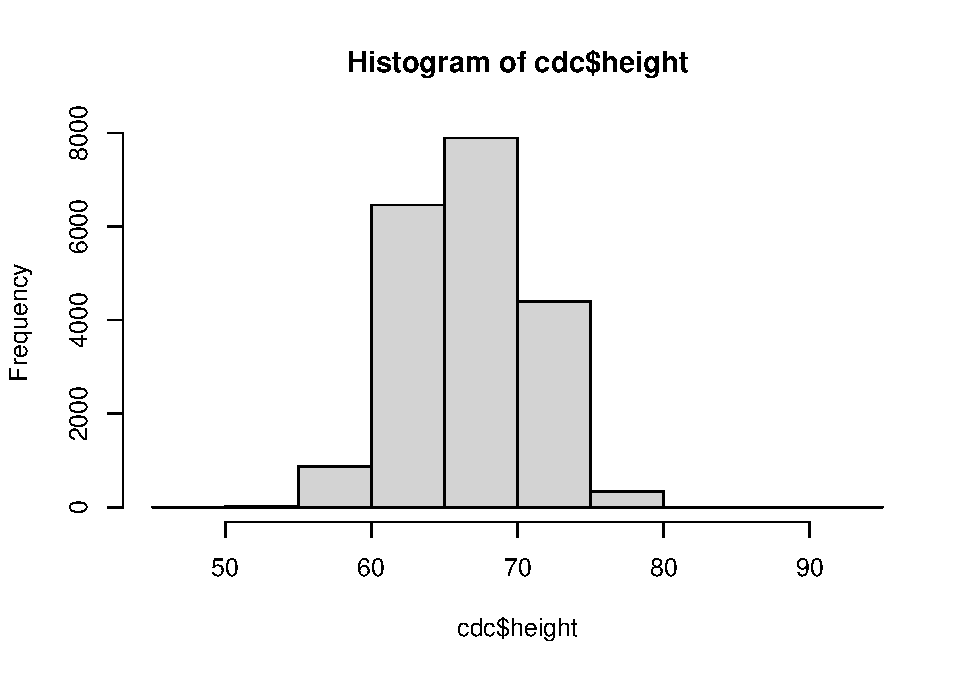
\includegraphics{_main_files/figure-latex/unnamed-chunk-123-1.pdf}

\begin{Shaded}
\begin{Highlighting}[]
\KeywordTok{hist}\NormalTok{(cdc}\OperatorTok{$}\NormalTok{weight)}
\end{Highlighting}
\end{Shaded}

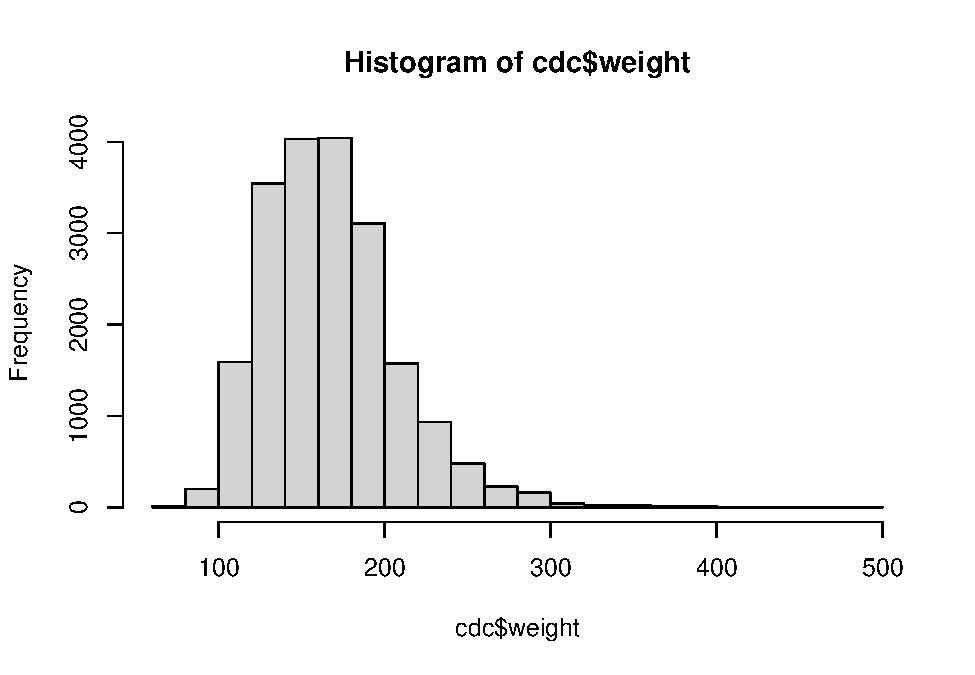
\includegraphics{_main_files/figure-latex/unnamed-chunk-123-2.pdf}

\begin{Shaded}
\begin{Highlighting}[]
\KeywordTok{hist}\NormalTok{(cdc}\OperatorTok{$}\NormalTok{age)}
\end{Highlighting}
\end{Shaded}

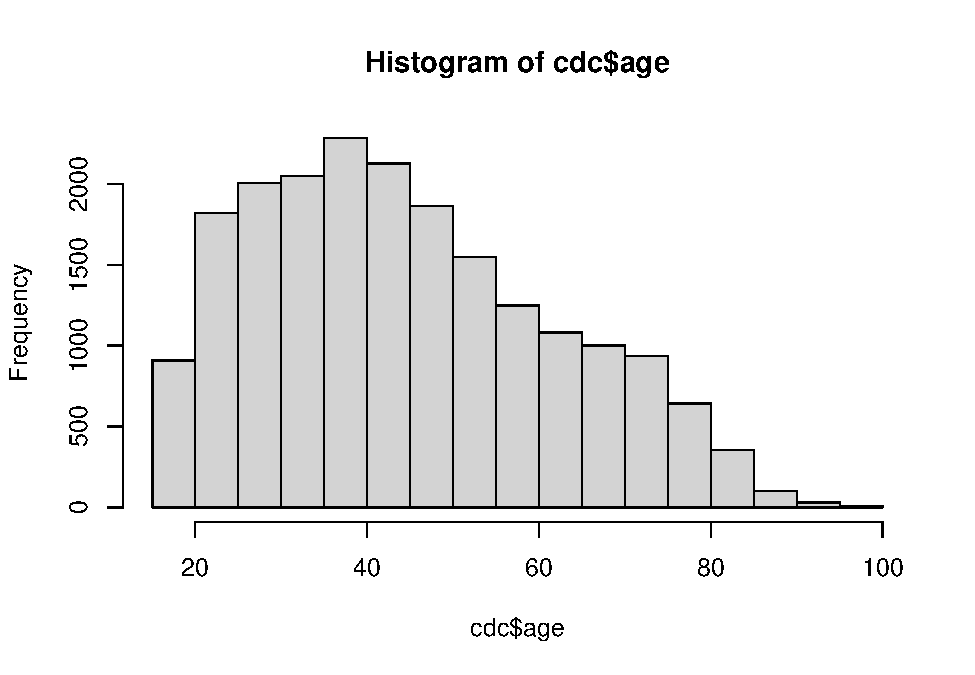
\includegraphics{_main_files/figure-latex/unnamed-chunk-123-3.pdf}

The output appears in the \emph{Plots} panel of \emph{RStudio}. You can use the arrows to the left of the \emph{Zoom} button the switch among the three plots.

\begin{Shaded}
\begin{Highlighting}[]
\KeywordTok{hist}\NormalTok{(cdc}\OperatorTok{$}\NormalTok{weight, }\DataTypeTok{breaks=}\DecValTok{20}\NormalTok{, }\DataTypeTok{main=}\StringTok{"Distribution of Weight"}\NormalTok{,}\DataTypeTok{xlab=}\StringTok{"Weight (kg)"}\NormalTok{)}
\end{Highlighting}
\end{Shaded}

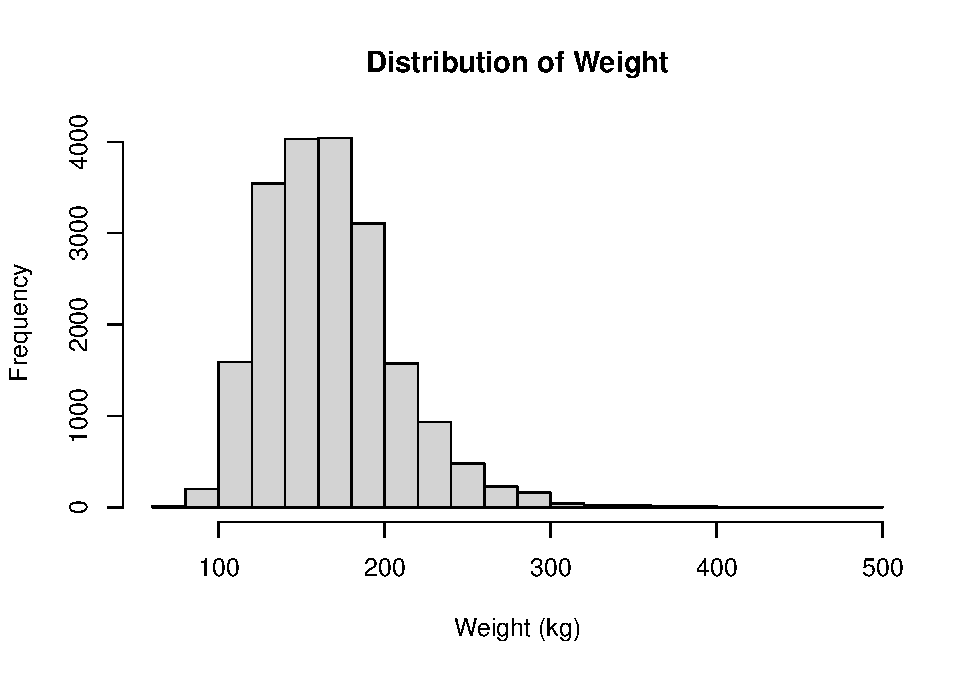
\includegraphics{_main_files/figure-latex/unnamed-chunk-124-1.pdf}

We specified that we want 20 cells for the histogram, added a main title, and title for the x-axis.

Use \texttt{col} argument to change the colors used for the bars. By using the \texttt{border} argument, you can even change the color used for the border of the bars.

\begin{Shaded}
\begin{Highlighting}[]
\KeywordTok{hist}\NormalTok{(cdc}\OperatorTok{$}\NormalTok{weight, }\DataTypeTok{breaks=}\DecValTok{20}\NormalTok{, }\DataTypeTok{main=}\StringTok{"Distribution of Weight"}\NormalTok{,}
     \DataTypeTok{xlab=}\StringTok{"Weight (kg)"}\NormalTok{, }
     \DataTypeTok{border =} \StringTok{"mediumpurple4"}\NormalTok{,}
     \DataTypeTok{col =} \StringTok{"mediumpurple1"}\NormalTok{)}
\end{Highlighting}
\end{Shaded}

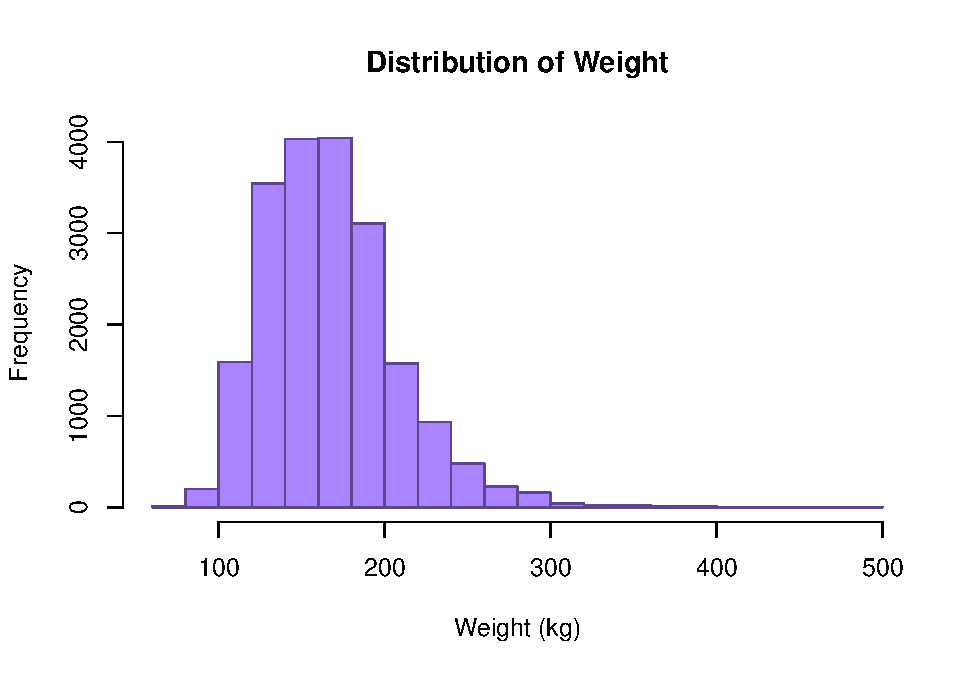
\includegraphics{_main_files/figure-latex/unnamed-chunk-125-1.pdf}

There are several ways we can add \textbf{colors} to \texttt{R}.

\begin{itemize}
\item
  \textbf{Using Color Names}: \texttt{R} programming has names for 657 colors. You can take a look at them all with the \texttt{colors()} function, or simply check this R color pdf.
\item
  \textbf{Using Hex Values as Colors}: Instead of using a color name, color can also be defined with a hexadecimal value. We define a color as a 6 hexadecimal digit number of the form \texttt{\#RRGGBB}. Where the \texttt{RR} is for red, \texttt{GG} for green and \texttt{BB} for blue and value ranges from \texttt{00} to \texttt{FF}. For example, \texttt{\#FF0000} would be red and \texttt{\#00FF00} would be green similarly, \#FFFFFF would be white and \texttt{\#000000} would be black.
\item
  \textbf{Using RGB Values} The function \texttt{rgb()} allows us to specify red, green and blue component with a number between 0 and 1. This function returns the corresponding hex code discussed above.
\item
  \textbf{Using a Color Palette}: R programming offers 5 built in color palettes which can be used to quickly generate color vectors of desired length. They are: \texttt{rainbow()}, \texttt{heat.colors()}, \texttt{terrain.colors()}, \texttt{topo.colors()} and \texttt{cm.colors()}. We pass in the number of colors that we want
\end{itemize}

Often you want to draw attention to specific values or observations in your graphic to provide unique insight. You can do this by adding markers to your graphic. For example, adding mean line will give you an idea about how much of the distribution is above and below the average. You can add such marker by using the \texttt{abline()} function.

\begin{Shaded}
\begin{Highlighting}[]
\KeywordTok{hist}\NormalTok{(cdc}\OperatorTok{$}\NormalTok{weight, }\DataTypeTok{breaks=}\DecValTok{20}\NormalTok{, }\DataTypeTok{main=}\StringTok{"Distribution of Weight"}\NormalTok{,}
     \DataTypeTok{xlab=}\StringTok{"Weight (kg)"}\NormalTok{, }
     \DataTypeTok{border =} \StringTok{"mediumpurple4"}\NormalTok{,}
     \DataTypeTok{col =} \StringTok{"mediumpurple1"}\NormalTok{)}

\KeywordTok{abline}\NormalTok{(}\DataTypeTok{v=}\KeywordTok{mean}\NormalTok{(cdc}\OperatorTok{$}\NormalTok{weight),}
       \DataTypeTok{col=}\StringTok{"mediumblue"}\NormalTok{,}
       \DataTypeTok{lty=}\DecValTok{2}\NormalTok{,}
       \DataTypeTok{lwd=}\DecValTok{2}\NormalTok{)}
\end{Highlighting}
\end{Shaded}

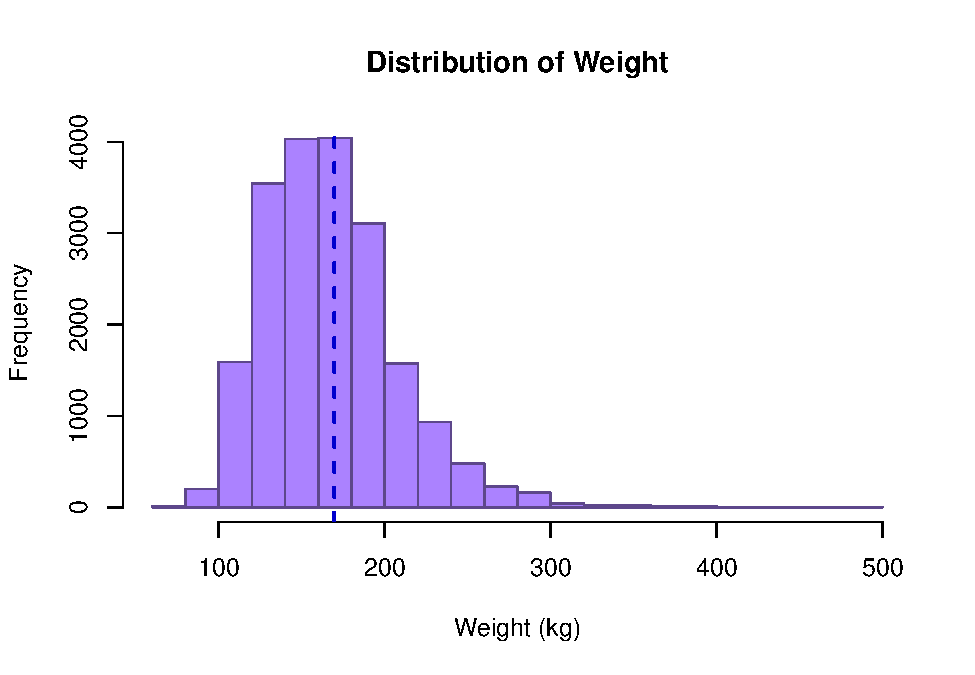
\includegraphics{_main_files/figure-latex/unnamed-chunk-126-1.pdf}

You can also place values on top of bars; which will help you interpret the graph correctly. You can add them by setting the labels argument to \texttt{TRUE}.

\begin{Shaded}
\begin{Highlighting}[]
\KeywordTok{hist}\NormalTok{(cdc}\OperatorTok{$}\NormalTok{height[}\DecValTok{1}\OperatorTok{:}\DecValTok{1000}\NormalTok{],}
     \DataTypeTok{col=}\StringTok{"dodgerblue3"}\NormalTok{,}
     \DataTypeTok{labels=}\OtherTok{TRUE}\NormalTok{, }
     \DataTypeTok{ylim =} \KeywordTok{c}\NormalTok{(}\DecValTok{0}\NormalTok{, }\DecValTok{200}\NormalTok{), }
     \DataTypeTok{breaks =} \DecValTok{18}\NormalTok{)}
\end{Highlighting}
\end{Shaded}

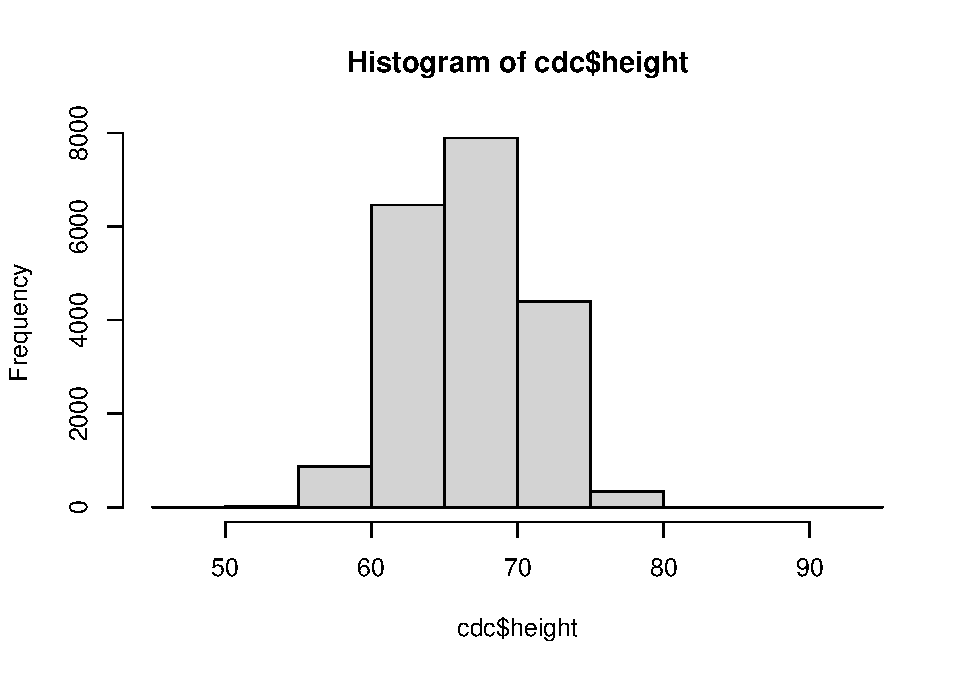
\includegraphics{_main_files/figure-latex/unnamed-chunk-127-1.pdf}

Often you want to compare the distributions of different variables within your data. You can overlay the histograms by setting the \texttt{add} argument of the second histogram to \texttt{TRUE}.

\begin{Shaded}
\begin{Highlighting}[]
\CommentTok{# random numbers}
\NormalTok{h1 =}\StringTok{ }\KeywordTok{rnorm}\NormalTok{(}\DecValTok{1000}\NormalTok{,}\DecValTok{6}\NormalTok{)}
\NormalTok{h2 =}\StringTok{ }\KeywordTok{rnorm}\NormalTok{(}\DecValTok{1000}\NormalTok{,}\DecValTok{4}\NormalTok{)}

\CommentTok{# Overlay two histograms}
\KeywordTok{hist}\NormalTok{(h1,}
     \DataTypeTok{col=}\KeywordTok{rgb}\NormalTok{(}\DecValTok{1}\NormalTok{,}\DecValTok{0}\NormalTok{,}\DecValTok{0}\NormalTok{,}\FloatTok{0.25}\NormalTok{))}
\KeywordTok{hist}\NormalTok{(h2,}
     \DataTypeTok{col=}\KeywordTok{rgb}\NormalTok{(}\DecValTok{0}\NormalTok{,}\DecValTok{0}\NormalTok{,}\DecValTok{1}\NormalTok{,}\FloatTok{0.25}\NormalTok{),}
     \DataTypeTok{add=}\OtherTok{TRUE}\NormalTok{)}
\end{Highlighting}
\end{Shaded}

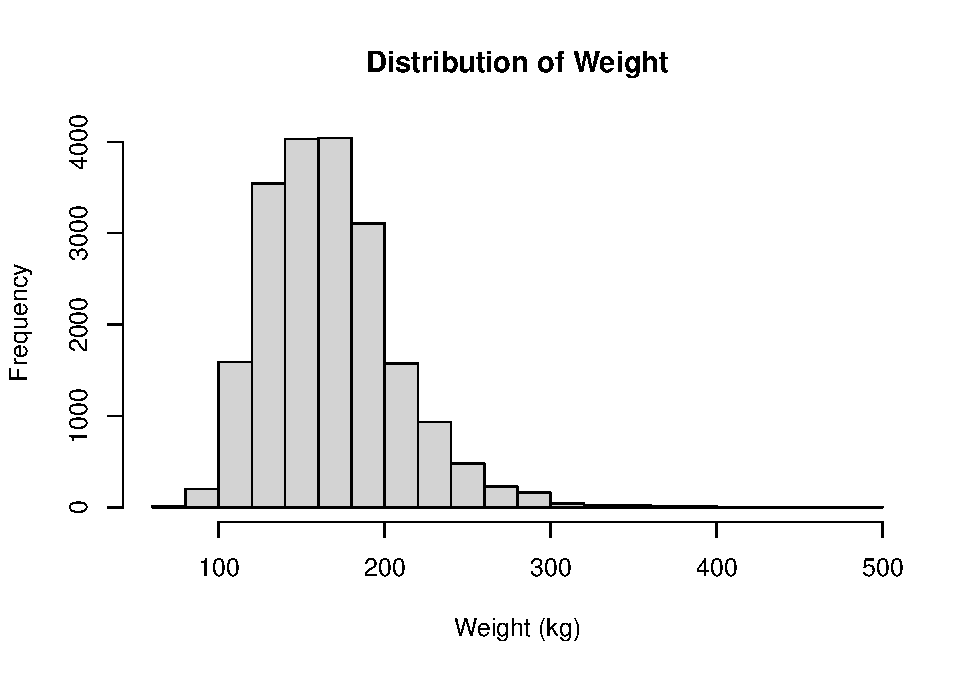
\includegraphics{_main_files/figure-latex/unnamed-chunk-128-1.pdf}

For more options, look up ``hist'' in the \emph{Help} panel of \emph{RStudio}.

Let's produce a boxplot for the first 1000 values of the height variable.

\begin{Shaded}
\begin{Highlighting}[]
\KeywordTok{boxplot}\NormalTok{(cdc}\OperatorTok{$}\NormalTok{height[}\DecValTok{1}\OperatorTok{:}\DecValTok{1000}\NormalTok{])}
\end{Highlighting}
\end{Shaded}

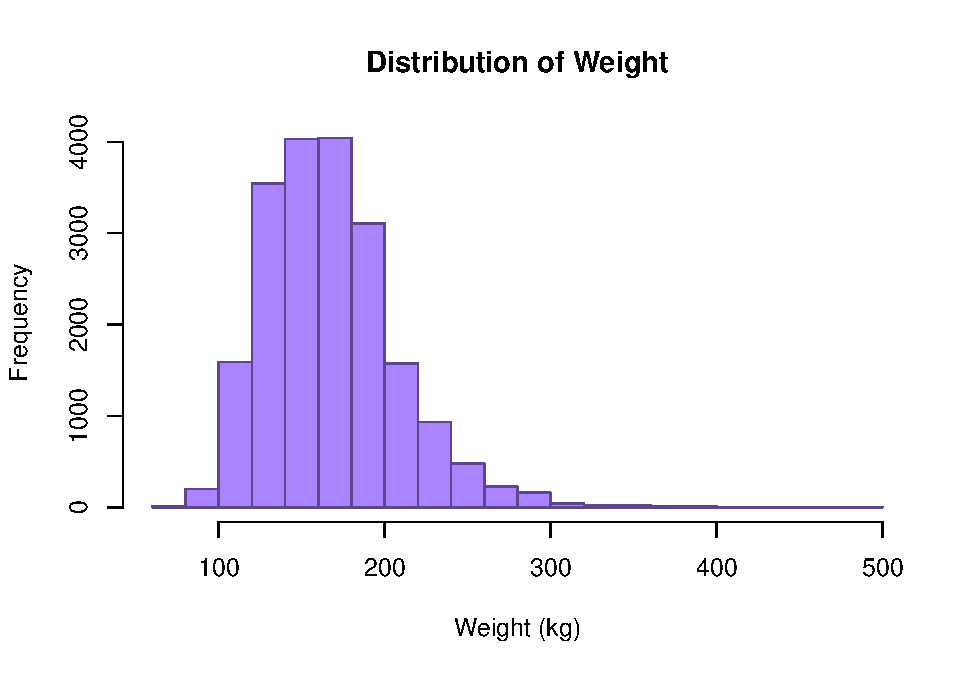
\includegraphics{_main_files/figure-latex/unnamed-chunk-129-1.pdf}

The line in the center is the median. The bottom and top of the box are drawn at the first (\(Q_1\)) and third (\(Q_3\)) quartiles (same as the 25th and 75th percentiles). The difference between the third and first quartiles is called the interquartile range (\(Q_3-Q_1\)). This is the height of the box. The lines above and below the box are called the whiskers. The upper whisker is either the third quartile plus 1.5 times the interquartile range, \(Q3 +1.5(Q_3-Q_1)\), or the largest data value, whichever is smallest. Similarly, the lower whisker is either the first quartile minus 1.5 times the interquartile range, \(Q1-1.5(Q_3-Q_1)\), or the smallest data value, whichever is largest. If data values exceed the whiskers, they are plotted as circles. Boxplots are often used to represent numeric data. One can use boxplots to compare different groups.

\begin{Shaded}
\begin{Highlighting}[]
\KeywordTok{boxplot}\NormalTok{(cdc}\OperatorTok{$}\NormalTok{height[}\DecValTok{1}\OperatorTok{:}\DecValTok{1000}\NormalTok{] }\OperatorTok{~}\StringTok{ }\NormalTok{cdc}\OperatorTok{$}\NormalTok{gender[}\DecValTok{1}\OperatorTok{:}\DecValTok{1000}\NormalTok{])}
\end{Highlighting}
\end{Shaded}

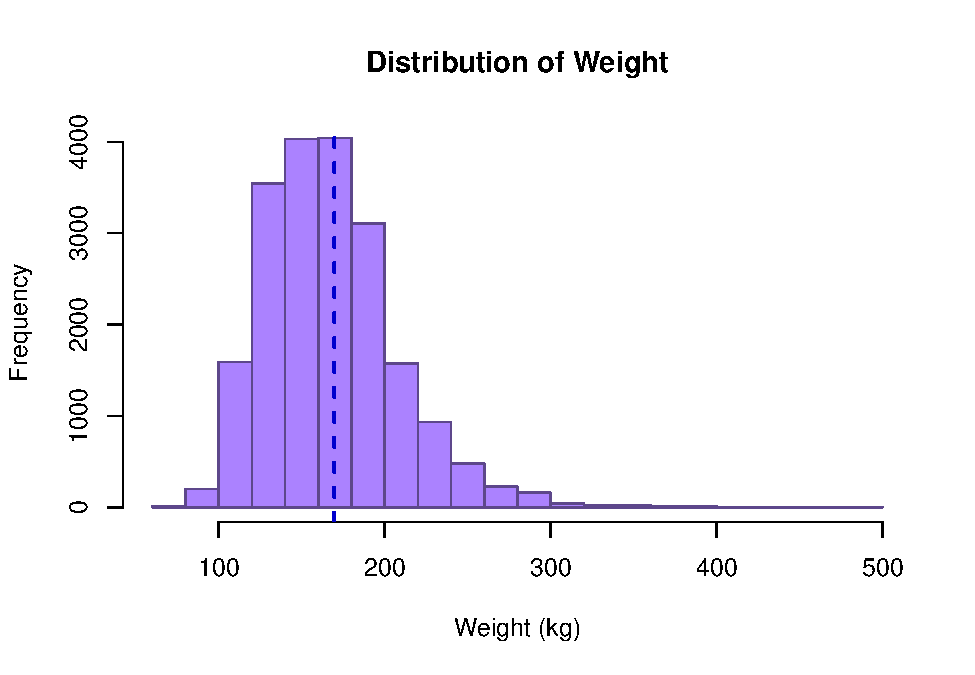
\includegraphics{_main_files/figure-latex/unnamed-chunk-130-1.pdf}

\hypertarget{visualizing-qualitative-data}{%
\section{Visualizing Qualitative Data}\label{visualizing-qualitative-data}}

We will now look at some of the qualitative data that are not numbers, but categories or groups. The \texttt{table()} function can be used to tabulate categorical data. The \texttt{genhlth} variable has five categories, we can use \texttt{table()} to find the frequencies.

\begin{Shaded}
\begin{Highlighting}[]
\KeywordTok{table}\NormalTok{(cdc}\OperatorTok{$}\NormalTok{genhlth)}
\end{Highlighting}
\end{Shaded}

\begin{verbatim}
## 
## excellent very good      good      fair      poor 
##      4657      6972      5675      2019       677
\end{verbatim}

Since the sample size is 20,000, we can divide by n to get proportions.

\begin{Shaded}
\begin{Highlighting}[]
\KeywordTok{table}\NormalTok{(cdc}\OperatorTok{$}\NormalTok{genhlth)}\OperatorTok{/}\DecValTok{20000}
\end{Highlighting}
\end{Shaded}

\begin{verbatim}
## 
## excellent very good      good      fair      poor 
##   0.23285   0.34860   0.28375   0.10095   0.03385
\end{verbatim}

Pie charts are also used for categorical data. Options are also available for the \texttt{pie()} function.

\begin{Shaded}
\begin{Highlighting}[]
\KeywordTok{pie}\NormalTok{(}\KeywordTok{table}\NormalTok{(cdc}\OperatorTok{$}\NormalTok{genhlth)}\OperatorTok{/}\DecValTok{20000}\NormalTok{)}
\end{Highlighting}
\end{Shaded}

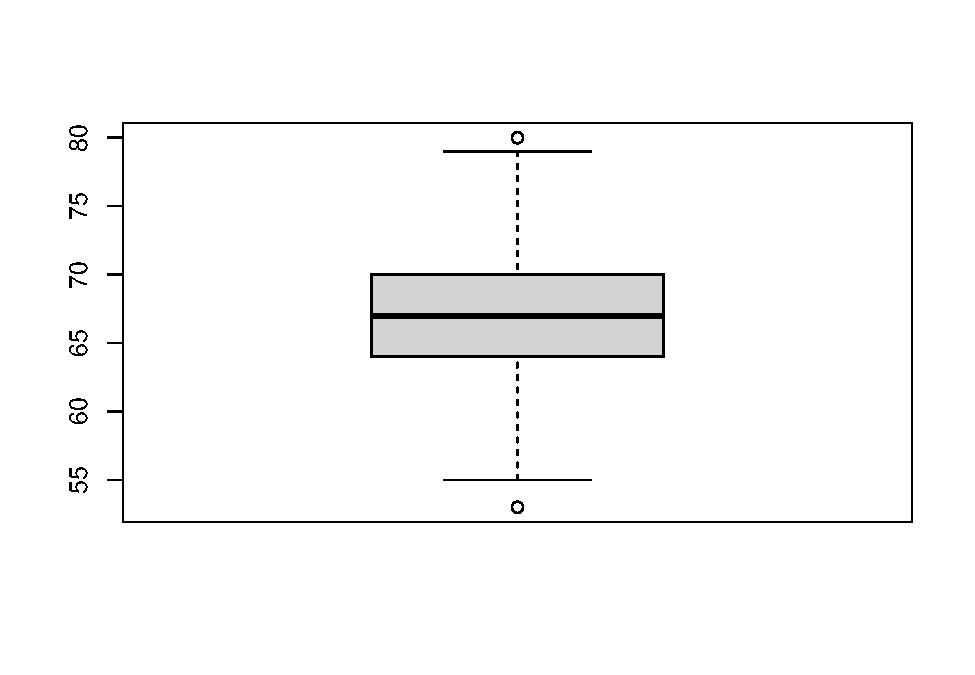
\includegraphics{_main_files/figure-latex/unnamed-chunk-133-1.pdf}

Options are also available for the pie() function.

\begin{Shaded}
\begin{Highlighting}[]
\NormalTok{colors =}\StringTok{ }\KeywordTok{c}\NormalTok{(}\StringTok{"green"}\NormalTok{, }\StringTok{"blue"}\NormalTok{, }\StringTok{"yellow"}\NormalTok{, }\StringTok{"pink"}\NormalTok{, }\StringTok{"red"}\NormalTok{)}
\KeywordTok{pie}\NormalTok{(}\KeywordTok{table}\NormalTok{(cdc}\OperatorTok{$}\NormalTok{genhlth)}\OperatorTok{/}\DecValTok{20000}\NormalTok{, }\DataTypeTok{col =}\NormalTok{ colors, }\DataTypeTok{main =} \StringTok{"General Health"}\NormalTok{)}
\end{Highlighting}
\end{Shaded}

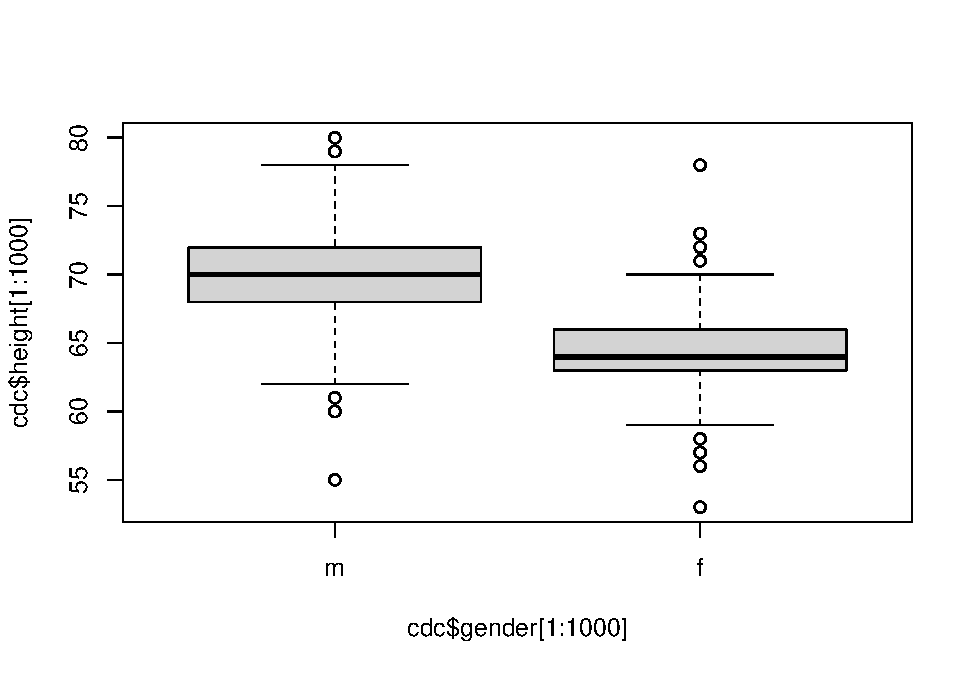
\includegraphics{_main_files/figure-latex/unnamed-chunk-134-1.pdf}

The \texttt{table()} function can also be used to cross-tabulate categorical data. Let's create a frequency table of smokers and non-smokers for both genders.

\begin{Shaded}
\begin{Highlighting}[]
\KeywordTok{table}\NormalTok{(cdc}\OperatorTok{$}\NormalTok{smoke100, cdc}\OperatorTok{$}\NormalTok{gender)}
\end{Highlighting}
\end{Shaded}

\begin{verbatim}
##    
##        m    f
##   0 4547 6012
##   1 5022 4419
\end{verbatim}

The zero is for nonsmokers and the one is for smokers. We can also create a frequency table of general health classifications for both genders.

\begin{Shaded}
\begin{Highlighting}[]
\KeywordTok{table}\NormalTok{(cdc}\OperatorTok{$}\NormalTok{genhlth, cdc}\OperatorTok{$}\NormalTok{gender)}
\end{Highlighting}
\end{Shaded}

\begin{verbatim}
##            
##                m    f
##   excellent 2298 2359
##   very good 3382 3590
##   good      2722 2953
##   fair       884 1135
##   poor       283  394
\end{verbatim}

\hypertarget{packages}{%
\chapter{Packages}\label{packages}}

\texttt{R} packages are a collection of \texttt{R} functions, complied code and sample data. They are stored under a directory called ``library'' in the \texttt{R} environment. By default, \texttt{R} installs a set of packages during installation. More packages are added later, when they are needed for some specific purpose. When we start the \texttt{R} console, only the default packages are available by default. Other packages which are already installed have to be loaded explicitly to be used by the \texttt{R} program that is going to use them.

All the packages available in \texttt{R} language are listed at \href{https://cran.r-project.org/web/packages/available_packages_by_name.html}{R Packages}.

To see a list of all packages installed on your device.

\begin{Shaded}
\begin{Highlighting}[]
\KeywordTok{library}\NormalTok{()}
\end{Highlighting}
\end{Shaded}

To see a list of all packages that are currently loaded.

\begin{Shaded}
\begin{Highlighting}[]
\KeywordTok{search}\NormalTok{()}
\end{Highlighting}
\end{Shaded}

\begin{verbatim}
##  [1] ".GlobalEnv"        "package:xtable"    "package:knitr"    
##  [4] "package:stats"     "package:graphics"  "package:grDevices"
##  [7] "package:utils"     "package:datasets"  "package:methods"  
## [10] "Autoloads"         "package:base"
\end{verbatim}

When adding a new package to our library we only have to install it once. We can do so with the following command.

\begin{Shaded}
\begin{Highlighting}[]
\KeywordTok{install.packages}\NormalTok{(}\StringTok{"library name"}\NormalTok{)}
\end{Highlighting}
\end{Shaded}

Alternatively, we can also go to the lower left hand window and select the \emph{Packages} tab. Then hit the button \textbf{Install}. A dropdown menu will appear where we can search for the package name.

Before a package can be used in the code, it must be loaded to the current R environment. You also need to load a package that is already installed previously but not available in the current environment.

\begin{Shaded}
\begin{Highlighting}[]
\KeywordTok{library}\NormalTok{(}\StringTok{"library name"}\NormalTok{)}
\end{Highlighting}
\end{Shaded}

For example, suppose we wanted to install and load the package ``ggplot2'', (a very popular package for making plots). We would type the following commands.

\begin{Shaded}
\begin{Highlighting}[]
\CommentTok{# Install package (only need to do this once)}
\KeywordTok{install.packages}\NormalTok{(}\StringTok{"ggplot2"}\NormalTok{)}

\CommentTok{# Load into working environment (need to do this for each new R session)}
\KeywordTok{library}\NormalTok{(}\StringTok{"ggplot2"}\NormalTok{)}
\end{Highlighting}
\end{Shaded}

\hypertarget{loops}{%
\chapter{Loops}\label{loops}}

\hypertarget{while-loop}{%
\section{While Loop}\label{while-loop}}

A while loop is used when you want to perform a task indefinitely, until a particular condition is met. It's a condition-controlled loop.

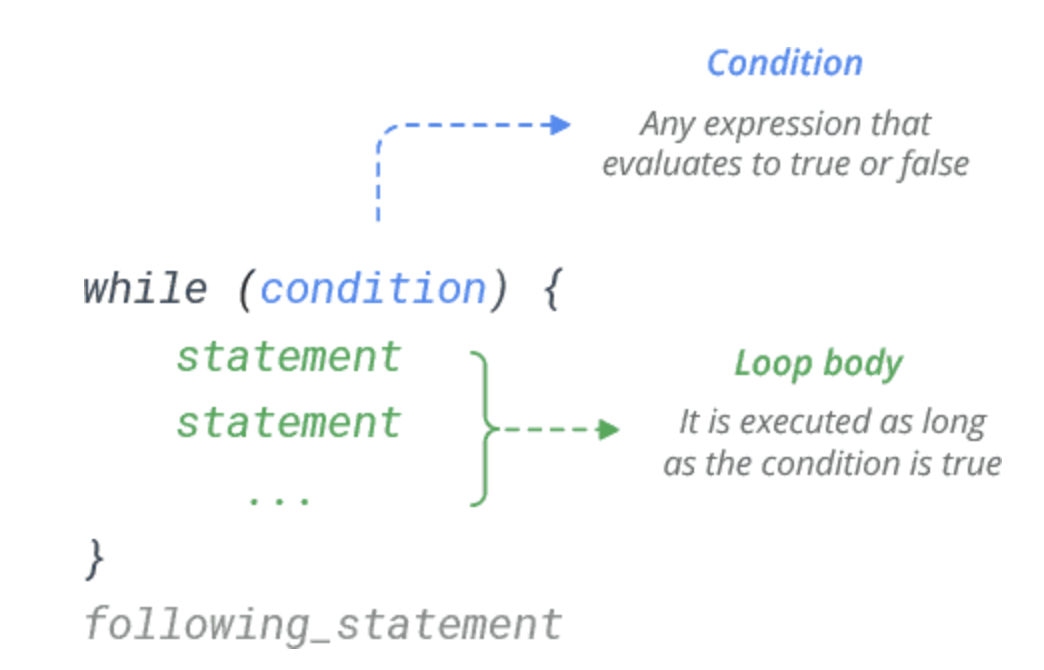
\includegraphics[width=14.5in]{images/WhileLoop}

The loop will continue until the condition is \texttt{FALSE}.

\begin{Shaded}
\begin{Highlighting}[]
\NormalTok{x =}\StringTok{ }\DecValTok{5}

\CommentTok{# If statement is true, keep running the loop }
\ControlFlowTok{while}\NormalTok{ (x }\OperatorTok{!=}\StringTok{ }\DecValTok{0}\NormalTok{ ) \{}
  \KeywordTok{print}\NormalTok{(x)}
\NormalTok{  x =}\StringTok{ }\NormalTok{x }\OperatorTok{-}\StringTok{ }\DecValTok{1}
\NormalTok{\}}
\end{Highlighting}
\end{Shaded}

\begin{verbatim}
## [1] 5
## [1] 4
## [1] 3
## [1] 2
## [1] 1
\end{verbatim}

If the condition is false at the start, the while loop will never be executed at all.

\begin{Shaded}
\begin{Highlighting}[]
\NormalTok{x =}\StringTok{ }\DecValTok{0}

\CommentTok{# If statement starts as TRUE,  the loop will never run }
\ControlFlowTok{while}\NormalTok{ (x }\OperatorTok{!=}\StringTok{ }\DecValTok{0}\NormalTok{ ) \{}
  \KeywordTok{print}\NormalTok{(x)}
\NormalTok{  x =}\StringTok{ }\NormalTok{x }\OperatorTok{-}\StringTok{ }\DecValTok{1}
\NormalTok{\}}
\end{Highlighting}
\end{Shaded}

The \texttt{break} statement is used to exit the loop immediately. It simply jumps out of the loop altogether, and the program continues after the loop.

\begin{Shaded}
\begin{Highlighting}[]
\NormalTok{x =}\StringTok{ }\DecValTok{5}

\CommentTok{# If statement starts as TRUE,  the loop will never run }
\ControlFlowTok{while}\NormalTok{ (x }\OperatorTok{!=}\StringTok{ }\DecValTok{0}\NormalTok{ ) \{}
  \KeywordTok{print}\NormalTok{(x)}
\NormalTok{  x =}\StringTok{ }\NormalTok{x }\OperatorTok{-}\StringTok{ }\DecValTok{1}
  
  \ControlFlowTok{if}\NormalTok{(x }\OperatorTok{==}\StringTok{ }\DecValTok{2}\NormalTok{)\{}
    \KeywordTok{print}\NormalTok{(}\StringTok{"Entered IF statement, stop loop"}\NormalTok{)}
    \ControlFlowTok{break} 
\NormalTok{  \}}
  
\NormalTok{\}}
\end{Highlighting}
\end{Shaded}

\begin{verbatim}
## [1] 5
## [1] 4
## [1] 3
## [1] "Entered IF statement, stop loop"
\end{verbatim}

If not given an adequate stopping criteria or break statement the loop will continue forever. For example, if we started the above examples at \texttt{x\ =\ -2}.

\hypertarget{for-loops}{%
\section{For Loops}\label{for-loops}}

The \texttt{for} statement in \texttt{R} is a bit different from what you usually use in other programming languages. Rather than iterating over a numeric progression, \texttt{R}'s \texttt{for} statement iterates over the items of a vector or a list. The items are iterated in the order that they appear in the vector.

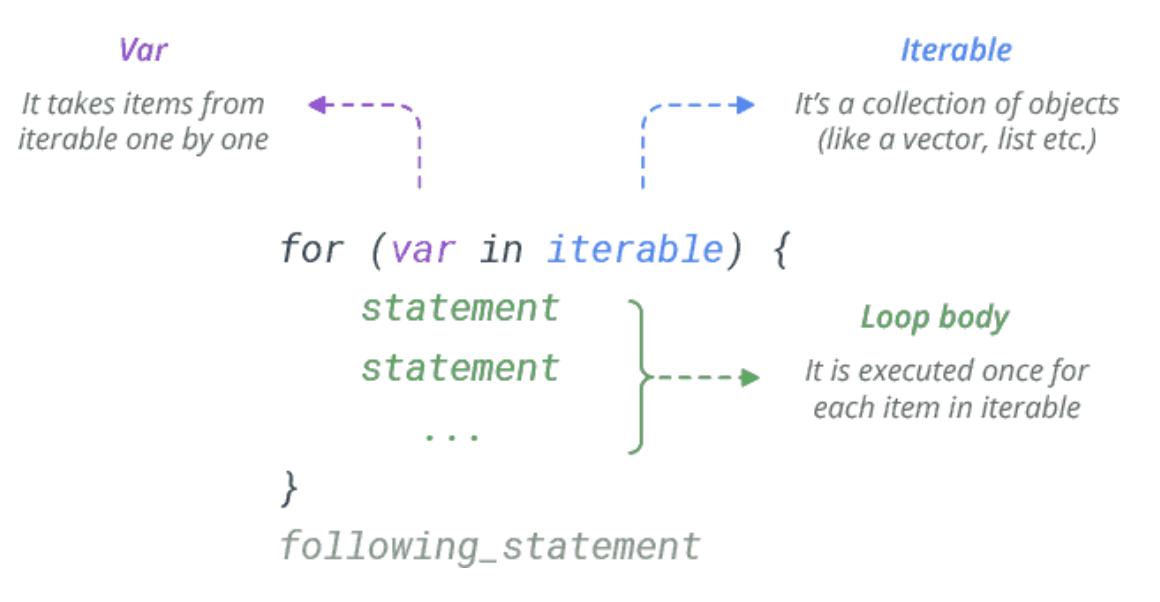
\includegraphics[width=16.11in]{images/ForLoop}

\begin{Shaded}
\begin{Highlighting}[]
\CommentTok{# Iterate through a vector}
\NormalTok{colors =}\StringTok{ }\KeywordTok{c}\NormalTok{(}\StringTok{"red"}\NormalTok{,}\StringTok{"green"}\NormalTok{,}\StringTok{"blue"}\NormalTok{,}\StringTok{"yellow"}\NormalTok{)}

\ControlFlowTok{for}\NormalTok{ (x }\ControlFlowTok{in}\NormalTok{ colors) \{}
  \KeywordTok{print}\NormalTok{(x)}
\NormalTok{\}}
\end{Highlighting}
\end{Shaded}

\begin{verbatim}
## [1] "red"
## [1] "green"
## [1] "blue"
## [1] "yellow"
\end{verbatim}

\begin{Shaded}
\begin{Highlighting}[]
\NormalTok{lst =}\StringTok{ }\KeywordTok{list}\NormalTok{(}\FloatTok{3.14}\NormalTok{, }\StringTok{"Hi"}\NormalTok{, }\KeywordTok{c}\NormalTok{(}\DecValTok{1}\NormalTok{,}\DecValTok{2}\NormalTok{,}\DecValTok{3}\NormalTok{))}

\ControlFlowTok{for}\NormalTok{ (i }\ControlFlowTok{in}\NormalTok{ lst) \{}
  \KeywordTok{print}\NormalTok{(i)}
\NormalTok{\}}
\end{Highlighting}
\end{Shaded}

\begin{verbatim}
## [1] 3.14
## [1] "Hi"
## [1] 1 2 3
\end{verbatim}

If you need to execute a group of statements for a specified number of times, use sequence operator : or built-in function \texttt{seq()}.

\begin{Shaded}
\begin{Highlighting}[]
\CommentTok{# Print 'Hello!' 3 times}
\ControlFlowTok{for}\NormalTok{ (x }\ControlFlowTok{in} \DecValTok{1}\OperatorTok{:}\DecValTok{3}\NormalTok{) \{}
  \KeywordTok{print}\NormalTok{(}\StringTok{"Hello!"}\NormalTok{)}
\NormalTok{\}}
\end{Highlighting}
\end{Shaded}

\begin{verbatim}
## [1] "Hello!"
## [1] "Hello!"
## [1] "Hello!"
\end{verbatim}

\begin{Shaded}
\begin{Highlighting}[]
\ControlFlowTok{for}\NormalTok{ (x }\ControlFlowTok{in} \KeywordTok{seq}\NormalTok{(}\DataTypeTok{from=}\DecValTok{2}\NormalTok{,}\DataTypeTok{to=}\DecValTok{8}\NormalTok{,}\DataTypeTok{by=}\DecValTok{2}\NormalTok{)) \{}
  \KeywordTok{print}\NormalTok{(x}\OperatorTok{^}\DecValTok{2}\NormalTok{)}
\NormalTok{\}}
\end{Highlighting}
\end{Shaded}

\begin{verbatim}
## [1] 4
## [1] 16
## [1] 36
## [1] 64
\end{verbatim}

Like the while loop, the \texttt{break} statement is used to exit the loop immediately. It simply jumps out of the loop altogether, and the program continues after the loop.

\begin{Shaded}
\begin{Highlighting}[]
\NormalTok{colors =}\StringTok{ }\KeywordTok{c}\NormalTok{(}\StringTok{"red"}\NormalTok{,}\StringTok{"green"}\NormalTok{,}\StringTok{"blue"}\NormalTok{,}\StringTok{"yellow"}\NormalTok{)}
\ControlFlowTok{for}\NormalTok{ (x }\ControlFlowTok{in}\NormalTok{ colors) \{}
  \ControlFlowTok{if}\NormalTok{ (x }\OperatorTok{==}\StringTok{ "blue"}\NormalTok{)\{}
       \ControlFlowTok{break} 
\NormalTok{  \}}
  \KeywordTok{print}\NormalTok{(x)}
\NormalTok{\}}
\end{Highlighting}
\end{Shaded}

\begin{verbatim}
## [1] "red"
## [1] "green"
\end{verbatim}

For loops do not have the same risk of ``running forever'', like while loops have.

\hypertarget{bisection}{%
\section{Bisection}\label{bisection}}

\hypertarget{nested-loops}{%
\section{Nested Loops}\label{nested-loops}}

\hypertarget{switch}{%
\section{Switch}\label{switch}}

\hypertarget{next}{%
\section{Next}\label{next}}

\hypertarget{break}{%
\section{Break}\label{break}}

\hypertarget{practice-problems}{%
\section*{Practice Problems}\label{practice-problems}}
\addcontentsline{toc}{section}{Practice Problems}

\begin{enumerate}
\def\labelenumi{\arabic{enumi})}
\item
  Create the function which has one arguement \texttt{n}. Have this function generate the first n fibannaci numbers using a \textbf{while} loop. Note that the Fibanacci sequence is formed by starting with the number 0, 1 and then adding the last two numbers to get the next number: 0, 1, 1, 2, 3, 5, 8, etc.
\item
  Create the function which has one arguement \texttt{n}. Have this function generate the first n fibannaci numbers using a \textbf{for} loop. Note that the Fibanacci sequence is formed by starting with the number 0, 1 and then adding the last two numbers to get the next number: 0, 1, 1, 2, 3, 5, 8, etc.
\item
  Create a function which has one argument \texttt{num}. Have this function generate the factorial of this number using any iteration technique you would like. Recall that a factorial of a number is product of all whole numbers from our chosen number down to 1. For example, 4! (4 factorial) = 4(3)(2)(1) = 24
\item
  Write a function which has only one argument \texttt{n}. Have this function display the \texttt{n} terms of odd natural number and their sum.
\end{enumerate}

\textbf{Answer 1}

\begin{Shaded}
\begin{Highlighting}[]
\CommentTok{# Generate the first n fibannaci numbers}

\NormalTok{gen_fib =}\StringTok{ }\ControlFlowTok{function}\NormalTok{(n)\{}

  \CommentTok{# Initiate the fib sequence }
\NormalTok{  fib =}\StringTok{ }\KeywordTok{c}\NormalTok{(}\DecValTok{0}\NormalTok{,}\DecValTok{1}\NormalTok{)}
\NormalTok{  current_n =}\StringTok{ }\KeywordTok{length}\NormalTok{(fib)}
  
  \ControlFlowTok{while}\NormalTok{(current_n}\OperatorTok{<}\NormalTok{n)\{}
    \CommentTok{# Generate the next number }
\NormalTok{    next_number =}\StringTok{ }\NormalTok{fib[}\KeywordTok{c}\NormalTok{(current_n}\DecValTok{-1}\NormalTok{)] }\OperatorTok{+}\StringTok{ }\NormalTok{fib[current_n]}
    
    \CommentTok{# Add new number }
\NormalTok{    fib =}\StringTok{ }\KeywordTok{c}\NormalTok{(fib, next_number)}
    
    \CommentTok{# Update the length }
\NormalTok{    current_n =}\StringTok{ }\KeywordTok{length}\NormalTok{(fib)}
\NormalTok{  \}}
  
  \KeywordTok{return}\NormalTok{(fib)}
\NormalTok{\}}
\end{Highlighting}
\end{Shaded}

\textbf{Answer 2}

\begin{Shaded}
\begin{Highlighting}[]
\CommentTok{# Generate the first n fibannaci numbers}

\NormalTok{gen_fib =}\StringTok{ }\ControlFlowTok{function}\NormalTok{(n)\{}

  \CommentTok{# Initiate the fib sequence}
\NormalTok{  fib =}\StringTok{ }\KeywordTok{c}\NormalTok{(}\DecValTok{0}\NormalTok{,}\DecValTok{1}\NormalTok{, }\KeywordTok{rep}\NormalTok{(}\DecValTok{0}\NormalTok{, }\KeywordTok{c}\NormalTok{(n}\DecValTok{-2}\NormalTok{)))}
  
  \ControlFlowTok{for}\NormalTok{(index }\ControlFlowTok{in} \DecValTok{3}\OperatorTok{:}\KeywordTok{length}\NormalTok{(fib))\{}
    \CommentTok{# Generate the next number }
\NormalTok{    next_number =}\StringTok{ }\NormalTok{fib[}\KeywordTok{c}\NormalTok{(index}\DecValTok{-2}\NormalTok{)] }\OperatorTok{+}\StringTok{ }\NormalTok{fib[index}\DecValTok{-1}\NormalTok{]}
    
    \CommentTok{# Add new number }
\NormalTok{    fib[index] =}\StringTok{ }\NormalTok{next_number}
\NormalTok{  \}}
  
  \KeywordTok{return}\NormalTok{(fib)}
\NormalTok{\}}
\end{Highlighting}
\end{Shaded}

\textbf{Answer 3}

\begin{Shaded}
\begin{Highlighting}[]
\NormalTok{my_factorial =}\StringTok{ }\ControlFlowTok{function}\NormalTok{(num)\{}
\NormalTok{  my_answer =}\StringTok{ }\DecValTok{1}
  \ControlFlowTok{for}\NormalTok{(i }\ControlFlowTok{in} \DecValTok{1}\OperatorTok{:}\NormalTok{num)\{}
\NormalTok{    my_answer =}\StringTok{ }\NormalTok{my_answer }\OperatorTok{*}\StringTok{ }\NormalTok{i }
\NormalTok{  \}}
  \KeywordTok{print}\NormalTok{(my_answer)}
\NormalTok{\}}
\end{Highlighting}
\end{Shaded}

\textbf{Answer 4}

\begin{Shaded}
\begin{Highlighting}[]
\NormalTok{odd_numbers =}\StringTok{ }\ControlFlowTok{function}\NormalTok{(n)\{}
\NormalTok{    odd_vector =}\StringTok{ }\OtherTok{NA}
  
  \ControlFlowTok{for}\NormalTok{(i }\ControlFlowTok{in} \DecValTok{1}\OperatorTok{:}\NormalTok{n)\{}
\NormalTok{    odd_vector[i] =}\StringTok{ }\DecValTok{2}\OperatorTok{*}\NormalTok{i }\OperatorTok{-}\StringTok{ }\DecValTok{1}
\NormalTok{  \}}
    
\NormalTok{ return_me =}\StringTok{ }\KeywordTok{list}\NormalTok{(}\DataTypeTok{vector =}\NormalTok{ odd_vector, }
                  \DataTypeTok{the_sum =} \KeywordTok{sum}\NormalTok{(odd_vector))}
 \KeywordTok{return}\NormalTok{(return_me)}
\NormalTok{\}}

\KeywordTok{odd_numbers}\NormalTok{(}\DecValTok{5}\NormalTok{)}
\end{Highlighting}
\end{Shaded}

\begin{verbatim}
## $vector
## [1] 1 3 5 7 9
## 
## $the_sum
## [1] 25
\end{verbatim}

\hypertarget{apply-family-of-functions}{%
\chapter{Apply Family of Functions}\label{apply-family-of-functions}}

Loops (like \texttt{for}, and \texttt{while}) are a way to repeatedly execute some code. However, they are often slow in execution when it comes to processing large data sets.

\texttt{R} has a more efficient and quick approach to perform iterations -- \textbf{The apply family}.

The apply family consists of vectorized functions. Below are the most common forms of apply functions.

\begin{itemize}
\tightlist
\item
  \texttt{apply()}
\item
  \texttt{lapply()}
\item
  \texttt{sapply()}
\item
  \texttt{tapply()}
\end{itemize}

These functions let you take data in batches and process the whole batch at once.

There primary difference is in the object (such as list, matrix, data frame etc.) on which the function is applied to and the object that will be returned from the function.

\hypertarget{apply-function}{%
\section{apply() function}\label{apply-function}}

The \texttt{apply()}function is used to apply a function to the rows or columns of matrices or data frames. It assembles the returned values into a vector, and then returns that vector.

If you want to apply a function on a data frame, make sure that the data frame is homogeneous (i.e.~either all numeric values or all character strings) Otherwise, R will force all columns to have identical types. This may not be what you want. In that case, use the \texttt{lapply()} or \texttt{sapply()} functions.

Description of the required \texttt{apply()} arguments:

\begin{itemize}
\tightlist
\item
  \texttt{X}: A matrix , data frame or array
\item
  \texttt{MARGIN}: A vector giving the subscripts which the function will be applied over.

  \begin{itemize}
  \tightlist
  \item
    1 indicates rows
  \item
    2 indicates columns
  \item
    c(1, 2) indicates rows and columns
  \end{itemize}
\item
  \texttt{FUN}: The function to be applied
\end{itemize}

\begin{Shaded}
\begin{Highlighting}[]
\CommentTok{# Get column means }
\NormalTok{data =}\StringTok{ }\KeywordTok{matrix}\NormalTok{(}\DecValTok{1}\OperatorTok{:}\DecValTok{9}\NormalTok{, }\DataTypeTok{nrow=}\DecValTok{3}\NormalTok{, }\DataTypeTok{ncol=}\DecValTok{3}\NormalTok{)}
\NormalTok{data}
\end{Highlighting}
\end{Shaded}

\begin{verbatim}
##      [,1] [,2] [,3]
## [1,]    1    4    7
## [2,]    2    5    8
## [3,]    3    6    9
\end{verbatim}

\begin{Shaded}
\begin{Highlighting}[]
\KeywordTok{apply}\NormalTok{(data, }\DecValTok{2}\NormalTok{, mean)}
\end{Highlighting}
\end{Shaded}

\begin{verbatim}
## [1] 2 5 8
\end{verbatim}

\begin{Shaded}
\begin{Highlighting}[]
\CommentTok{# Get row means }
\KeywordTok{apply}\NormalTok{(data, }\DecValTok{1}\NormalTok{, sum)}
\end{Highlighting}
\end{Shaded}

\begin{verbatim}
## [1] 12 15 18
\end{verbatim}

You can use user-defined functions as well.

\begin{Shaded}
\begin{Highlighting}[]
\KeywordTok{apply}\NormalTok{(data, }\DecValTok{2}\NormalTok{, }\ControlFlowTok{function}\NormalTok{(x)\{}
  
  \CommentTok{# Standard deviation formula }
\NormalTok{  y =}\StringTok{ }\KeywordTok{sum}\NormalTok{(x }\OperatorTok{-}\KeywordTok{mean}\NormalTok{(x))}\OperatorTok{^}\DecValTok{2}\OperatorTok{/}\NormalTok{(}\KeywordTok{length}\NormalTok{(x)}\OperatorTok{-}\DecValTok{1}\NormalTok{)}
  
  \KeywordTok{return}\NormalTok{(y)}
\NormalTok{  \})}
\end{Highlighting}
\end{Shaded}

\begin{verbatim}
## [1] 0 0 0
\end{verbatim}

\hypertarget{lapply-function}{%
\section{lapply() function}\label{lapply-function}}

The \texttt{lapply()} function is used to apply a function to each element of the list. It collects the returned values into a list, and then \textbf{returns that list}.

Description of the required \texttt{lapply()} arguments:

\begin{itemize}
\tightlist
\item
  \texttt{X}: A matrix , data frame or array
\item
  \texttt{FUN}: The function to be applied
\end{itemize}

\begin{Shaded}
\begin{Highlighting}[]
\NormalTok{data_lst =}\StringTok{ }\KeywordTok{list}\NormalTok{(}\DataTypeTok{item1 =} \DecValTok{1}\OperatorTok{:}\DecValTok{5}\NormalTok{,}
             \DataTypeTok{item2 =} \KeywordTok{seq}\NormalTok{(}\DecValTok{4}\NormalTok{,}\DecValTok{36}\NormalTok{,}\DecValTok{8}\NormalTok{),}
             \DataTypeTok{item3 =} \KeywordTok{c}\NormalTok{(}\DecValTok{1}\NormalTok{,}\DecValTok{3}\NormalTok{,}\DecValTok{5}\NormalTok{,}\DecValTok{7}\NormalTok{,}\DecValTok{9}\NormalTok{))}
\NormalTok{data_lst }
\end{Highlighting}
\end{Shaded}

\begin{verbatim}
## $item1
## [1] 1 2 3 4 5
## 
## $item2
## [1]  4 12 20 28 36
## 
## $item3
## [1] 1 3 5 7 9
\end{verbatim}

\begin{Shaded}
\begin{Highlighting}[]
\NormalTok{data_vector =}\StringTok{ }\KeywordTok{c}\NormalTok{(}\DecValTok{1}\NormalTok{,}\DecValTok{2}\NormalTok{,}\DecValTok{3}\NormalTok{,}\DecValTok{4}\NormalTok{,}\DecValTok{5}\NormalTok{,}\DecValTok{6}\NormalTok{,}\DecValTok{7}\NormalTok{,}\DecValTok{8}\NormalTok{)}
\NormalTok{data_vector}
\end{Highlighting}
\end{Shaded}

\begin{verbatim}
## [1] 1 2 3 4 5 6 7 8
\end{verbatim}

\begin{Shaded}
\begin{Highlighting}[]
\KeywordTok{lapply}\NormalTok{(data_lst, sum)}
\end{Highlighting}
\end{Shaded}

\begin{verbatim}
## $item1
## [1] 15
## 
## $item2
## [1] 100
## 
## $item3
## [1] 25
\end{verbatim}

\begin{Shaded}
\begin{Highlighting}[]
\KeywordTok{lapply}\NormalTok{(data_vector, sum)}
\end{Highlighting}
\end{Shaded}

\begin{verbatim}
## [[1]]
## [1] 1
## 
## [[2]]
## [1] 2
## 
## [[3]]
## [1] 3
## 
## [[4]]
## [1] 4
## 
## [[5]]
## [1] 5
## 
## [[6]]
## [1] 6
## 
## [[7]]
## [1] 7
## 
## [[8]]
## [1] 8
\end{verbatim}

\hypertarget{sapply-function}{%
\section{sapply() function}\label{sapply-function}}

The \texttt{sapply()} and \texttt{lapply()} work basically the same.

The only difference is that \texttt{lapply()} always returns a list, whereas \texttt{sapply()} tries to simplify the result into a vector or matrix.

\begin{itemize}
\item
  If the return value is a list where every element is length 1, you get a vector.
\item
  If the return value is a list where every element is a vector of the same length (\textgreater{} 1), you get a matrix.
\item
  If the lengths vary, simplification is impossible and you get a list.
\end{itemize}

Description of the required \texttt{sapply()} arguments:

\begin{itemize}
\tightlist
\item
  \texttt{X}: A matrix , data frame or array
\item
  \texttt{FUN}: The function to be applied
\end{itemize}

\begin{Shaded}
\begin{Highlighting}[]
\NormalTok{data_lst =}\StringTok{ }\KeywordTok{list}\NormalTok{(}\DataTypeTok{item1 =} \DecValTok{1}\OperatorTok{:}\DecValTok{5}\NormalTok{,}
                 \DataTypeTok{item2 =} \KeywordTok{seq}\NormalTok{(}\DecValTok{4}\NormalTok{,}\DecValTok{36}\NormalTok{,}\DecValTok{8}\NormalTok{),}
                 \DataTypeTok{item3 =} \KeywordTok{c}\NormalTok{(}\DecValTok{1}\NormalTok{,}\DecValTok{3}\NormalTok{,}\DecValTok{5}\NormalTok{,}\DecValTok{7}\NormalTok{,}\DecValTok{9}\NormalTok{))}
\NormalTok{data_lst}
\end{Highlighting}
\end{Shaded}

\begin{verbatim}
## $item1
## [1] 1 2 3 4 5
## 
## $item2
## [1]  4 12 20 28 36
## 
## $item3
## [1] 1 3 5 7 9
\end{verbatim}

\begin{Shaded}
\begin{Highlighting}[]
\KeywordTok{sapply}\NormalTok{(data_lst, sum)}
\end{Highlighting}
\end{Shaded}

\begin{verbatim}
## item1 item2 item3 
##    15   100    25
\end{verbatim}

\hypertarget{tapply-function}{%
\section{tapply() function}\label{tapply-function}}

The \texttt{tapply()} function breaks the data set up into groups and applies a function to each group.

Description of the required \texttt{sapply()} arguments:

\begin{itemize}
\tightlist
\item
  \texttt{X}: A matrix , data frame or array
\item
  \texttt{INDEX}: A grouping factor or a list of factors
\item
  \texttt{FUN}: The function to be applied
\end{itemize}

\begin{Shaded}
\begin{Highlighting}[]
\NormalTok{data =}\StringTok{ }\KeywordTok{data.frame}\NormalTok{(}\DataTypeTok{name=}\KeywordTok{c}\NormalTok{(}\StringTok{"Amy"}\NormalTok{,}\StringTok{"Max"}\NormalTok{,}\StringTok{"Ray"}\NormalTok{,}\StringTok{"Kim"}\NormalTok{,}\StringTok{"Sam"}\NormalTok{,}\StringTok{"Eve"}\NormalTok{,}\StringTok{"Bob"}\NormalTok{), }
                  \DataTypeTok{age=}\KeywordTok{c}\NormalTok{(}\DecValTok{24}\NormalTok{, }\DecValTok{22}\NormalTok{, }\DecValTok{21}\NormalTok{, }\DecValTok{23}\NormalTok{, }\DecValTok{20}\NormalTok{, }\DecValTok{24}\NormalTok{, }\DecValTok{21}\NormalTok{),}
                  \DataTypeTok{gender=}\KeywordTok{factor}\NormalTok{(}\KeywordTok{c}\NormalTok{(}\StringTok{"F"}\NormalTok{,}\StringTok{"M"}\NormalTok{,}\StringTok{"M"}\NormalTok{,}\StringTok{"F"}\NormalTok{,}\StringTok{"M"}\NormalTok{,}\StringTok{"F"}\NormalTok{,}\StringTok{"M"}\NormalTok{))) }

\NormalTok{data}
\end{Highlighting}
\end{Shaded}

\begin{verbatim}
##   name age gender
## 1  Amy  24      F
## 2  Max  22      M
## 3  Ray  21      M
## 4  Kim  23      F
## 5  Sam  20      M
## 6  Eve  24      F
## 7  Bob  21      M
\end{verbatim}

\begin{Shaded}
\begin{Highlighting}[]
\KeywordTok{tapply}\NormalTok{(data}\OperatorTok{$}\NormalTok{age, data}\OperatorTok{$}\NormalTok{gender, min)}
\end{Highlighting}
\end{Shaded}

\begin{verbatim}
##  F  M 
## 23 20
\end{verbatim}

\hypertarget{practice-problems-1}{%
\section*{Practice Problems}\label{practice-problems-1}}
\addcontentsline{toc}{section}{Practice Problems}

\begin{enumerate}
\def\labelenumi{\arabic{enumi})}
\tightlist
\item
  Using one of the apply functions (\texttt{apply(),\ lapply,\ sapply(),} or \texttt{tapply()}), recreate the results that the \texttt{summary()} function produces for the built-in data set \texttt{mtcars}.
\end{enumerate}

\begin{Shaded}
\begin{Highlighting}[]
\KeywordTok{summary}\NormalTok{(mtcars)}
\end{Highlighting}
\end{Shaded}

\begin{verbatim}
##       mpg             cyl             disp             hp       
##  Min.   :10.40   Min.   :4.000   Min.   : 71.1   Min.   : 52.0  
##  1st Qu.:15.43   1st Qu.:4.000   1st Qu.:120.8   1st Qu.: 96.5  
##  Median :19.20   Median :6.000   Median :196.3   Median :123.0  
##  Mean   :20.09   Mean   :6.188   Mean   :230.7   Mean   :146.7  
##  3rd Qu.:22.80   3rd Qu.:8.000   3rd Qu.:326.0   3rd Qu.:180.0  
##  Max.   :33.90   Max.   :8.000   Max.   :472.0   Max.   :335.0  
##       drat             wt             qsec             vs        
##  Min.   :2.760   Min.   :1.513   Min.   :14.50   Min.   :0.0000  
##  1st Qu.:3.080   1st Qu.:2.581   1st Qu.:16.89   1st Qu.:0.0000  
##  Median :3.695   Median :3.325   Median :17.71   Median :0.0000  
##  Mean   :3.597   Mean   :3.217   Mean   :17.85   Mean   :0.4375  
##  3rd Qu.:3.920   3rd Qu.:3.610   3rd Qu.:18.90   3rd Qu.:1.0000  
##  Max.   :4.930   Max.   :5.424   Max.   :22.90   Max.   :1.0000  
##        am              gear            carb      
##  Min.   :0.0000   Min.   :3.000   Min.   :1.000  
##  1st Qu.:0.0000   1st Qu.:3.000   1st Qu.:2.000  
##  Median :0.0000   Median :4.000   Median :2.000  
##  Mean   :0.4062   Mean   :3.688   Mean   :2.812  
##  3rd Qu.:1.0000   3rd Qu.:4.000   3rd Qu.:4.000  
##  Max.   :1.0000   Max.   :5.000   Max.   :8.000
\end{verbatim}

\begin{enumerate}
\def\labelenumi{\arabic{enumi})}
\setcounter{enumi}{1}
\tightlist
\item
  Retry Homework 4 using \emph{apply(), lapply, sapply(),} and \emph{tapply()} functions.
\end{enumerate}

\newpage

\textbf{Answer 1}

\begin{Shaded}
\begin{Highlighting}[]
\NormalTok{my_summary =}\StringTok{ }\KeywordTok{apply}\NormalTok{(mtcars, }\DecValTok{2}\NormalTok{, }\ControlFlowTok{function}\NormalTok{(column)\{}
  
  \CommentTok{# Min}
\NormalTok{  the_min =}\StringTok{ }\KeywordTok{min}\NormalTok{(column)}
  
  \CommentTok{# First Qurtile}
\NormalTok{  the_Q1 =}\StringTok{ }\KeywordTok{quantile}\NormalTok{(column, }\FloatTok{.25}\NormalTok{)}
  
  \CommentTok{# Median}
\NormalTok{  the_median =}\StringTok{ }\KeywordTok{median}\NormalTok{(column)}
  
  \CommentTok{# Mean }
\NormalTok{  the_mean =}\StringTok{ }\KeywordTok{mean}\NormalTok{(column)}
  
  \CommentTok{# Third Quartile}
\NormalTok{  the_Q3 =}\StringTok{ }\KeywordTok{quantile}\NormalTok{(column, }\FloatTok{.75}\NormalTok{)}
  
  \CommentTok{# Max}
\NormalTok{  the_max =}\StringTok{ }\KeywordTok{max}\NormalTok{(column)}
  
  \CommentTok{# Return values}
\NormalTok{  return_me =}\StringTok{ }\KeywordTok{c}\NormalTok{(the_min, the_Q1, the_median,}
\NormalTok{                the_mean, the_Q3, the_max)}
  \KeywordTok{names}\NormalTok{(return_me) =}\StringTok{ }\KeywordTok{c}\NormalTok{(}\StringTok{"Min.:"}\NormalTok{, }\StringTok{"1st Qu.:"}\NormalTok{, }
                       \StringTok{"Median:"}\NormalTok{, }\StringTok{"Mean:"}\NormalTok{, }
                       \StringTok{"3rd Qu.:"}\NormalTok{, }\StringTok{"Max.:"}\NormalTok{)}
  
  \KeywordTok{return}\NormalTok{(return_me)}
\NormalTok{\})}

\NormalTok{my_summary}
\end{Highlighting}
\end{Shaded}

\begin{verbatim}
##               mpg    cyl     disp       hp     drat      wt     qsec     vs
## Min.:    10.40000 4.0000  71.1000  52.0000 2.760000 1.51300 14.50000 0.0000
## 1st Qu.: 15.42500 4.0000 120.8250  96.5000 3.080000 2.58125 16.89250 0.0000
## Median:  19.20000 6.0000 196.3000 123.0000 3.695000 3.32500 17.71000 0.0000
## Mean:    20.09062 6.1875 230.7219 146.6875 3.596563 3.21725 17.84875 0.4375
## 3rd Qu.: 22.80000 8.0000 326.0000 180.0000 3.920000 3.61000 18.90000 1.0000
## Max.:    33.90000 8.0000 472.0000 335.0000 4.930000 5.42400 22.90000 1.0000
##               am   gear   carb
## Min.:    0.00000 3.0000 1.0000
## 1st Qu.: 0.00000 3.0000 2.0000
## Median:  0.00000 4.0000 2.0000
## Mean:    0.40625 3.6875 2.8125
## 3rd Qu.: 1.00000 4.0000 4.0000
## Max.:    1.00000 5.0000 8.0000
\end{verbatim}

  \bibliography{book.bib,packages.bib}

\end{document}
